%!LW recipe=latexmk-report

% -*- coding: utf-8 -*-

% \documentclass[12pt, a4paper, titlepage]{article}
\documentclass[language=fr, year=2A, enterprise=ensIIE]{ensiie-report}

%%%%%%%%%%%%%%%%%%%%%%%%%%%%%%%%%%%%%%%%
%%%%%%% DÉCLARATION DU PRÉAMBULE %%%%%%%
%%%%%%%%%%%%%%%%%%%%%%%%%%%%%%%%%%%%%%%%

\usepackage{preamble}

%%%%%%%%%%%%%%%%%%%%%%%%%%%%%%%%%%%%%%%%
%%%%%%% DÉCLARATION DU GLOSSAIRE %%%%%%%
%%%%%%%%%%%%%%%%%%%%%%%%%%%%%%%%%%%%%%%%

\makeglossaries
% -*- coding: utf-8 -*-
% !TEX root = main.tex

\newglossaryentry{pruning}
{
    name={pruning},
    description={Élagage d'un réseau neuronal par suppression de paramètres ou de structures jugés peu utiles}
}

\newglossaryentry{sparsity}
{
    name={sparsité},
    description={Proportion de coefficients annulés dans un ensemble de poids}
}

\newacronym{nlp}{NLP}{Natural Language Processing}
\newacronym{bpe}{BPE}{Byte Pair Encoding}
\newacronym{obd}{OBD}{Optimal Brain Damage}
\newacronym{obs}{OBS}{Optimal Brain Surgeon}
\newacronym{mint}{MINT}{Mutual Information-based Neuron Trimming}
\newacronym{gmi}{GMI}{Geometric Mutual Information}
\newacronym{mst}{MST}{Minimum Spanning Tree}
\newacronym{mac}{MAC}{Multiply--Accumulate}
\newacronym{flop}{FLOP}{Floating-Point Operation}


%%%%%%%%%%%%%%%%%%%%%%%%%%%%%%%%%%%%%%%%
% ACTIVATION DE L'EXTERNALISATION TIKZ %
%%%%%%%%%%%%%%%%%%%%%%%%%%%%%%%%%%%%%%%%

% On le fait pas dans le fichier .sty car c'est une commande qui dépend de documentclass.
% En clair, cela va permettre de créer les images TikZ dans le dossier "tikz/build" pour gagner du temps de compilation (si jamais on est amené à en faire)
% La première compilation est très longue, celles qui suivent sont théoriquement plus rapides.

% Externalisation intéressante SI vous créez un certain nombre de figures avec TikZ. Si ce n'est pas le cas, vous pouvez laisser commenter les lignes suivantes pour la désactiver.

% /!\ L'externalisation ne fonctionne pas sur Overleaf.

% \tikzexternalize
% [
%     prefix=tikz/build/,
%     up to date check={md5},
%     optimize command away=\AddToShipoutPictureBG
% ] % Chemin du dossier qui contient les graphiques TikZ

%%%%%%%%%%%%%%%%%%%%%%%%%%%%%%%%%%%%
%%%%%%%%%%%% MÉTADONNÉES %%%%%%%%%%%%
%%%%%%%%%%%%%%%%%%%%%%%%%%%%%%%%%%%%%

%%%%%%%%
%%% TODO
%%% Standard macros
\title{Compression de modèles de classifications de sentiments de textes} % Sujet du stage
\author{Mohamed KASSOUL} % Prénom NOM de l'étudiant(e)
\date{Mecredi 1er juillet 2026 au mardi 25 août 2026} % Dates du stage
%%%%%%%

%%%%%%%%
%%% TODO
%%% Custom macros, à commenter si :
%%% - template utilisé pour autre chose qu'un rapport de stage
%%% - classe [ensiie-report] non utilisée
% \subtitle{Sous-titre} % Sous-titre facultatif, pour préciser le sujet ou l'écrire dans une autre langue
\years{2026-2027} % Année scolaire en cours
\logoSchool{img/logo_ensiie.png} % Chemin vers le logo de l'ensIIE (ex : img/logo_ensiie.png)
\logoEnterprise{img/ensiie_campus.jpg} % Chemin vers le logo de l'entreprise du stage (ex : img/logo_entreprise.png)
\academicSupervisor{Mathilde MOUGEOT} % Tuteur de stage
\internshipSupervisor{Mounir ATIQ} % Maître de stage
\internshipEnterprise{ensIIE (Évry-Courcouronnes, Essonne)} % Lieu du stage
%%%%%%%%

%%%%%%%%%%%%%%%%%%%%%%%%%%%%%%%%%%%%%%%
%%%%%%%%%% DÉBUT DU DOCUMENT %%%%%%%%%%
%%%%%%%%%%%%%%%%%%%%%%%%%%%%%%%%%%%%%%%

\begin{document}

\hypersetup{pageanchor=false}

% \newgeometry{hmargin=2.5cm,vmargin=2.5cm} % Changer les marges de la page de garde
\AddToShipoutPictureBG{\BackgroundPicFirstPage} % Pour activer le remplissage de la première page par le background choisi (dépend de l'entreprise définie dans la classe ensiie-report)
\maketitle
\ClearShipoutPictureBG % Pour retirer le fond sur toutes les pages suivantes
\afterpage{\blankpage} % Page vide
\restoregeometry

% \AddToShipoutPicture{\BackgroundPicAllPages} % Pour un autre fond sur toutes les autres pages

%%%%%%%%%%%%%%%%%%%%%%%%%%%%%%%%
%%%%%%%% REMERCIEMENTS %%%%%%%%%
%%%%%%%%%%%%%%%%%%%%%%%%%%%%%%%%

\pagenumbering{roman}
\hypersetup{pageanchor=true}
\pagestyle{FirstPages}

\section*{Remerciements}\label{sec:remerciements}
\addcontentsline{toc}{section}{Remerciements}

% -*- coding: utf-8 -*-
% !TEX root = ../main.tex

% TODO Vos remerciements (collègues de travail, famille, autre...)

Je tiens tout d’abord à exprimer ma profonde gratitude à Monsieur Mounir Atiq , chercheur au CEA et enseignant en analyse de données, pour son engagement déterminant dès l'origine de ce projet. Je le remercie chaleureusement d'avoir rendu ce stage possible en soutenant son montage auprès de l'administration malgré un calendrier serré lié à mon retour d'échange universitaire. Son accompagnement m'a été particulièrement précieux, tant par la richesse de ses apports intellectuels que par ses enseignements sur la structuration et la conduite rigoureuse d'un projet de recherche. Je lui suis sincèrement reconnaissant pour sa confiance, ses orientations méthodologiques et sa grande disponibilité tout au long de ces deux mois.

J'adresse également mes vifs remerciements à l'équipe du C19, l'incubateur de l'ensIIE, pour la mise à disposition de locaux de travail de qualité, offrant un cadre propice à nos recherches.

Mes remerciements s'adressent ensuite à ma tutrice académique, Mme Mathilde Mougeot, pour sa grande réactivité et son accompagnement dans les démarches administratives. Je remercie également le personnel administratif de l'ENSIIE pour son aide précieuse et son écoute au démarrage du stage pour finaliser les conventions.

Enfin, je tiens à remercier chaleureusement mes camarades de stage, Arnaud Grassian et Saad Rhouddal, pour les échanges stimulants, l'entraide technique et l'excellente ambiance de travail partagée au quotidien, ainsi que mes proches pour leurs relectures attentives et leur soutien.

\newpage

%%%%%%%%%%%%%%%%%%%%%%%%%%%%%%%%
%%%%%%%%%%% SYNTHÈSE %%%%%%%%%%%
%%%%%%%%%%%%%%%%%%%%%%%%%%%%%%%%

\section*{Synthèse}\label{sec:synthese}
\addcontentsline{toc}{section}{Synthèse}

% -*- coding: utf-8 -*-
% !TEX root = ../main.tex

% TODO Insérer la synthèse du stage

%%%
%%%

\paragraph*{Mots-clés}\label{par:mots-cles}

% TODO Mots-clés de votre rapport de stage

Template, rapport

\newpage

%%%%%%%%%%%%%%%%%%%%%%%%%%%%%%%%
%%%%%%%%%% GLOSSAIRE %%%%%%%%%%%
%%%%%%%%%%%%%%%%%%%%%%%%%%%%%%%%

\section*{Glossaire}\label{sec:glossaire}
\addcontentsline{toc}{section}{Glossaire}

\setglossarystyle{list}
% \setupglossaries{numberedsection=autolabel}
% \setupglossaries{section,numberedsection=nameref}
\printglossary[type=\acronymtype, title=Acronymes, toctitle=Acronymes]
\printglossary[title=Vocabulaire, toctitle=Vocabulaire]
\printglossary[type=symbol, toctitle=Symboles]
\newpage

%%%%%%%%%%%%%%%%%%%%%%%%%%%%%%%%%%%%%%%%%%%
%%% LISTES DES FIGURES/TABLES/ÉQUATIONS %%%
%%%%%%%%%%%%%%%%%%%%%%%%%%%%%%%%%%%%%%%%%%%

\renewcommand{\listfigurename}{Liste des figures}
\listoffigures\label{sec:lof}
\addcontentsline{toc}{section}{Liste des figures}
% \renewcommand{\listtablename}{Liste des tables}
% \listoftables\label{sec:lot}
% \addcontentsline{toc}{section}{Liste des tables}
% \renewcommand{\lstlistlistingname}{Liste des listings}
% \lstlistoflistings\label{sec:lol}
% \addcontentsline{toc}{section}{Liste des listings}
% \renewcommand{\listalgorithmcfname}{Liste des algorithmes}
% \listofalgorithms\label{sec:loa}
% \addcontentsline{toc}{section}{Liste des algorithmes}
\newpage

%%%%%%%%%%%%%%%%%%%%%%%%%%%%%%%%
%%%%%% TABLE DES MATIÈRES %%%%%%
%%%%%%%%%%%%%%%%%%%%%%%%%%%%%%%%

\renewcommand{\contentsname}{Table des matières}
\tableofcontents
\label{EndFirstPages} % Pour la numérotation en chiffre romain des premières pages
\newpage

%%%%%%%%%%%%%%%%%%%%%%%%%%%%%%%%
%%%%%%%%% INTRODUCTION %%%%%%%%%
%%%%%%%%%%%%%%%%%%%%%%%%%%%%%%%%

\pagenumbering{arabic}
\pagestyle{MainPages}

\section{Introduction}\label{sec:introduction}

% -*- coding: utf-8 -*-
% !TEX root = ../main.tex

\subsection{Organisme et équipe d'accueil}
\label{ssec:introduction_organisme}

Ce stage de recherche s'est déroulé au sein de l'École Nationale Supérieure d'Informatique pour l'Industrie et l'Entreprise (\textsc{ENSIIE}), et plus particulièrement dans les locaux du \textbf{C19}, l'incubateur d'entreprises et tiers-lieu d'innovation adossé à l'école. Cet environnement dédié à l'émergence de projets numériques et à l'émulation technologique a constitué un cadre propice pour mener des travaux expérimentaux et méthodologiques.

Le projet a été encadré par \textbf{M. Mounir Atiq}, chercheur au CEA et enseignant en analyse de données. L'activité de recherche s'est articulée autour de thématiques avancées en traitement automatique du langage naturel (\textit{Natural Language Processing} -- NLP), et plus précisément sur l'\textbf{analyse et la compression de sentiment de texte}. À l'heure où les modèles de langage de grande taille (\textit{Large Language Models} -- LLMs) et les architectures génératives transforment en profondeur l'état de l'art, les problématiques de représentations denses, d'efficacité algorithmique et de compression sémantique sont au cœur des défis scientifiques actuels.

Ce stage s'inscrit pleinement dans la continuité de ma spécialisation en apprentissage automatique (\textit{Machine Learning}) et intelligence artificielle durant mon cursus d'ingénieur. Il constitue une première expérience concrète dans le domaine de la recherche académique, renforçant ma rigueur méthodologique et théorique en vue de mon intégration prochaine au sein du Master 2 Mathématiques, Vision, Apprentissage (MVA).
\subsection{Contexte scientifique}
\label{ssec:introduction_contexte_scientifique}

La classification automatique de sentiments consiste à associer un texte à une
catégorie, par exemple un sentiment positif ou négatif. Les modèles neuronaux
utilisés pour cette tâche peuvent offrir de bonnes performances, mais leur coût
en mémoire et en calcul limite leur utilisation sur des ressources contraintes.
Ce travail étudie le compromis entre la qualité de prédiction et la complexité
d'une tête de classification neuronale obtenue après élagage de ses poids.

\subsection{Objectifs}
\label{ssec:introduction_objectifs}

L'objectif général est de construire un protocole reproductible permettant de :
\begin{itemize}
    \item entraîner un pipeline commun de représentation de textes et de
    classification de sentiments ;
    \item élaguer la tête de classification à l'aide de plusieurs méthodes de
    scoring ;
    \item mesurer la performance prédictive, la complexité mémoire et la
    complexité de calcul des modèles obtenus ;
    \item déterminer les modèles qui réalisent le meilleur compromis entre ces
    critères.
\end{itemize}

\subsection{Organisation du rapport}
\label{ssec:introduction_organisation}

Le cadre du travail est d'abord présenté, puis les motivations et l'état de
l'art introduisent les méthodes de pruning étudiées. La
\autoref{sec:formulation_probleme} définit les objets, les complexités et les
critères d'évaluation. La méthodologie décrit ensuite le protocole expérimental,
avant la présentation des résultats et des perspectives.

\newpage

%%%%%%%%%%%%%%%%%%%%%%%%%%%%%%%%
%%% MOTIVATIONS ET ÉTAT DE L'ART %%%
%%%%%%%%%%%%%%%%%%%%%%%%%%%%%%%%

\section{Motivations et état de l'art}\label{sec:motivations_etat_art}

% -*- coding: utf-8 -*-
% !TEX root = ../main.tex

La classification de texte est traversée par un compromis entre capacité
prédictive et coût d'utilisation. À famille d'architectures et conditions
d'apprentissage comparables, augmenter le nombre de paramètres élargit en
général la capacité d'un modèle à représenter des régularités complexes. Cette
augmentation ne garantit pas à elle seule une meilleure performance : son
intérêt dépend notamment des données disponibles et de l'optimisation. Elle a
néanmoins accompagné une grande partie des progrès récents, depuis les
représentations distribuées jusqu'aux modèles contextuels préentraînés.

Cette capacité supplémentaire a un coût. Un modèle plus volumineux occupe
davantage de mémoire et demande généralement plus d'opérations pour produire
une prédiction. Or l'entraînement peut n'être réalisé qu'une fois, tandis que
l'inférence est répétée pour chaque nouveau texte. Le coût pertinent pour le
déploiement n'est donc pas seulement celui de la construction du modèle, mais
aussi celui de son stockage et de son exécution répétée. La compression cherche
à réduire ce coût récurrent tout en limitant la dégradation de la performance.
Les travaux d'élagage s'inscrivent historiquement dans cette recherche d'une
capacité plus compacte \cite{lecun1989obd,han2015learning}.

Avant d'étudier cette compression, il faut préciser ce qui est effectivement
exécuté lors d'une classification. Le traitement comporte deux problèmes
successifs : transformer une suite de symboles, de longueur variable, en une
représentation numérique exploitable, puis prendre une décision à partir de
cette représentation. Dans un système neuronal, ces fonctions sont
généralement assurées par un \emph{backbone} de représentation et par une tête
de classification. Cette décomposition fournit le fil conducteur de l'état de
l'art : comprendre l'évolution de ces deux composants, les gains obtenus et les
coûts introduits, avant de présenter les méthodes proposées pour les réduire.

\subsection{Backbone de représentation et tête de classification}
\label{ssec:etat_art_architecture}

Le backbone reçoit le texte brut et produit les caractéristiques utilisées par
le classifieur. Il comprend d'abord une étape de tokenisation, qui découpe le
texte en unités et associe un identifiant à chacune d'elles. Il contient ensuite
un mécanisme de représentation. Dans un modèle fondé sur des embeddings, chaque
identifiant est associé à un vecteur dense de petite dimension appris à partir
des données. Le terme \emph{embedding} désigne à la fois cette association et
le vecteur obtenu. Enfin, lorsque le classifieur attend un seul vecteur par
texte, le backbone doit agréger les représentations des différentes unités, par
exemple au moyen d'une moyenne ou d'un réseau qui tient compte de leur ordre.

La tête de classification reçoit la représentation produite par le backbone et
la transforme en scores de classes. Elle peut être linéaire ou composée de
plusieurs couches. Dans le cas de l'analyse de sentiments binaire, elle doit
estimer si les caractéristiques du texte sont davantage associées à un
sentiment positif ou négatif. Son apprentissage utilise donc les textes
représentés par le backbone et leurs étiquettes, alors que le backbone peut être
préentraîné sur une tâche différente et éventuellement sans annotations de
sentiment.

Cette séparation permet aussi de distinguer le coût d'apprentissage du coût
d'inférence. Un backbone peut être préentraîné une fois, puis figé lorsque le
système est déployé. Classifier un nouveau texte ne demande alors pas de
réapprendre ses paramètres : le texte est propagé dans le backbone, puis dans
la tête, avec les paramètres déjà acquis. Le préentraînement constitue donc un
coût initial, tandis que les calculs d'inférence sont répétés à chaque
prédiction.

Le backbone et la tête peuvent tous deux être comprimés, mais ces deux choix
n'ont pas la même portée. Modifier le backbone peut réduire une part importante
du coût total, au risque de changer toutes les représentations fournies au
classifieur. Agir uniquement sur la tête laisse ces représentations inchangées
et isole le coût de la décision finale. Dans les deux cas, le fait qu'un
composant soit préentraîné ne le rend pas gratuit à l'inférence : il doit encore
être stocké et exécuté pour traiter une nouvelle entrée.

\subsection{Évolution des représentations et des classifieurs de texte}
\label{ssec:etat_art_representations}

Un algorithme d'apprentissage ne traite pas directement des mots ou des
caractères : il traite des nombres. La difficulté ne consiste donc pas seulement
à attribuer un identifiant à chaque unité, mais à construire une représentation
qui conserve les informations utiles à la tâche. Les méthodes successives se
distinguent par la nature de cette information et par le coût nécessaire pour
l'obtenir.

\subsubsection{Comptages, sacs de mots et séquences locales}

Une représentation simple est le sac de mots. Chaque coordonnée du vecteur
correspond à un élément du vocabulaire et contient son nombre d'occurrences, sa
présence ou un score TF--IDF, qui pondère la fréquence locale d'une unité par sa
rareté dans le corpus. Le texte est alors décrit par les unités qu'il contient,
indépendamment de leur position. Cette représentation est
facile à calculer et à interpréter, mais elle produit des vecteurs de la taille
du vocabulaire, généralement très creux. Surtout, elle ne porte aucune notion
de proximité : \emph{excellent} et \emph{remarquable} occupent deux coordonnées
indépendantes, même si ces mots peuvent exprimer une appréciation voisine.

Le sac de mots perd également l'ordre. Pour réintroduire un contexte local, il
est possible d'utiliser des $n$-grammes. Un $n$-gramme est une suite contiguë de
$n$ unités : un unigramme contient une unité, un bigramme en contient deux et
un trigramme trois. Les bigrammes peuvent par exemple distinguer la présence de
\emph{bon} de celle de \emph{pas bon}. Leur pouvoir descriptif a toutefois un
coût : le nombre de suites possibles augmente rapidement avec $n$ et avec la
taille du vocabulaire. La majorité des combinaisons sont rares ou absentes du
corpus, ce qui limite la généralisation à des formulations nouvelles.

Les travaux de Shannon fournissent le cadre probabiliste permettant de raisonner
sur ces séquences. Ils formalisent la source de symboles, l'entropie et la
dépendance statistique \cite{shannon1948communication}. Le
traité de Gallager systématise ensuite ces outils de théorie de l'information
\cite{gallager1968information}. Ces références ne proposent pas encore de
représentation sémantique des mots. Elles établissent plutôt les concepts qui
permettent de mesurer l'incertitude d'une séquence et l'information partagée par
ses éléments.

L'analyse distributionnelle apporte un changement de perspective. Harris
observe que le comportement d'une unité linguistique peut être étudié à partir
des environnements dans lesquels elle apparaît
\cite{harris1954distributional}. Autrement dit, les contextes d'un mot donnent
une information sur son rôle dans la langue. Cette idée permet de dépasser une
représentation où chaque mot est totalement indépendant des autres, sans encore
construire de vecteurs continus.

Brown et ses coauteurs exploitent cette information de contexte dans des
modèles de langage fondés sur des classes de mots
\cite{brown1992class}. Leur méthode regroupe les mots selon leurs statistiques
de cooccurrence et utilise ces groupes dans un modèle $n$-gramme. Les classes
obtenues peuvent refléter des régularités syntaxiques ou sémantiques, et elles
réduisent la rareté par rapport à un modèle où chaque mot est traité isolément.
La similarité reste cependant discrète : deux mots appartiennent ou non à la
même classe, sans que le modèle exprime différents degrés de proximité.

À ce stade, le backbone produit donc le plus souvent un vecteur de comptages,
éventuellement enrichi par des $n$-grammes, et la tête repose sur un algorithme
d'apprentissage classique. Le classifieur naïf bayésien estime la probabilité
d'une classe en supposant les caractéristiques conditionnellement
indépendantes. Le modèle de maximum d'entropie apprend directement une
distribution sur les classes sans cette hypothèse, tandis que la machine à
vecteurs de support recherche une frontière qui sépare les exemples avec une
marge aussi large que possible. Pang, Lee et Vaithyanathan comparent ces trois
familles sur la polarité de critiques de films
\cite{pang2002sentiment}. Leur étude confirme leur intérêt pour l'analyse de
sentiments, mais montre aussi que cette tâche est plus délicate que la
catégorisation thématique : la présence d'un mot positif ou négatif ne suffit
pas toujours, car sa portée, la négation et la construction de la phrase peuvent
en inverser l'interprétation.

Ces méthodes fournissent des bases solides et interprétables, mais elles restent
fortement liées aux formes effectivement observées. Deux expressions proches
partagent peu d'information si elles n'emploient pas les mêmes unités ou les
mêmes $n$-grammes. Il devient donc nécessaire de construire une représentation
qui encode des degrés de similarité plutôt que de simples identités.

\subsubsection{Passage aux représentations distribuées}

Bengio et ses coauteurs remplacent ces classes discrètes par des
représentations distribuées continues apprises avec un modèle de langage
neuronal \cite{bengio2003neural}. Leur point de départ est la malédiction de la
dimension : le nombre de séquences possibles est immense par rapport au nombre
de séquences réellement observées. Un modèle fondé sur l'appariement exact ne
sait donc pas bien traiter une combinaison nouvelle. Dans un espace continu,
une séquence inconnue peut au contraire bénéficier de ce qui a été appris sur
des séquences composées de mots proches. Si \emph{excellent} et
\emph{remarquable} apparaissent dans des environnements comparables, leurs
vecteurs peuvent ainsi devenir voisins et partager une partie de l'information
apprise. Le modèle apprend simultanément les vecteurs des mots et la fonction
qui prédit le mot suivant.

Cette continuité améliore la généralisation, mais introduit un nouveau coût :
pour chaque contexte, le réseau doit calculer une probabilité sur l'ensemble du
vocabulaire. Morin et Bengio proposent une
décomposition hiérarchique de cette distribution
\cite{morin2005hierarchical}. Le mot cible est atteint au terme d'une suite de
décisions dans une hiérarchie, ce qui réduit fortement le nombre de sorties à
évaluer. Leur contribution porte donc moins sur la définition de l'embedding
que sur la possibilité de l'apprendre à plus grande échelle.

Le modèle de Bengio utilise encore un contexte de longueur fixée avant
l'entraînement. Mikolov et ses coauteurs montrent qu'un réseau récurrent peut
conserver un état dépendant des mots précédents et exploiter ainsi une histoire
plus longue \cite{mikolov2010rnn}. Cette approche améliore la modélisation de la
séquence, mais son entraînement demeure relativement coûteux, notamment parce
que les états successifs sont dépendants les uns des autres. Si l'objectif
principal est d'obtenir de bons vecteurs de mots, il devient alors intéressant
de simplifier le modèle de langage lui-même.

\subsubsection{Word2Vec : apprendre efficacement à partir du contexte}

Word2Vec désigne une famille de modèles légers conçus pour apprendre des
représentations distribuées à partir des contextes observés dans un grand
corpus. Mikolov et ses coauteurs introduisent deux architectures
\cite{mikolov2013efficient}. Le modèle \emph{Continuous Bag-of-Words} (CBOW)
utilise les unités voisines pour prédire l'unité centrale. Skip-gram effectue la
tâche inverse : il part de l'unité centrale et cherche à prédire son contexte.
Par exemple, CBOW peut utiliser le contexte \emph{ce film est vraiment …} pour
prédire une unité telle que \emph{excellent}, alors que Skip-gram part de
\emph{excellent} pour apprendre à reconnaître les unités susceptibles de
l'entourer. Dans les deux cas, la tâche de prédiction sert de signal
d'apprentissage ; les vecteurs contenus dans la couche d'embedding sont ensuite
réutilisés dans d'autres applications.

Cette simplification ne résout pas entièrement le coût associé à un grand
vocabulaire. Mikolov et ses coauteurs proposent alors l'échantillonnage négatif,
ou \emph{negative sampling} \cite{mikolov2013distributed}. Plutôt que de
comparer systématiquement le mot cible à tous les éléments du vocabulaire,
l'entraînement oppose une association réellement observée à un petit nombre
d'associations artificielles. Le calcul devient beaucoup moins coûteux. Le
sous-échantillonnage des mots très fréquents évite en outre qu'ils dominent
l'apprentissage alors qu'ils sont souvent peu discriminants. Goldberg et Levy
reprennent ensuite cet objectif et en donnent une dérivation plus explicite
pour Skip-gram \cite{goldberg2014word2vec}. Leur analyse aide à comprendre que
l'échantillonnage négatif est un objectif d'apprentissage de représentations à
part entière, et pas uniquement une implémentation accélérée d'un modèle de
langage complet.

\subsubsection{Embeddings statiques et prise en compte de l'ordre}

Un embedding ainsi appris est dense et rapproche les unités apparaissant dans
des contextes similaires. Pour classifier un texte, la solution la plus simple
consiste à agréger ses embeddings, puis à fournir le vecteur obtenu à une tête
neuronale, par exemple un perceptron multicouche. Cette architecture est rapide
et sépare clairement le backbone de la tête. Elle ne peut toutefois pas
récupérer l'ordre perdu pendant l'agrégation : approfondir uniquement la tête ne
corrige donc pas les limites de la représentation qui lui est fournie.

Les architectures suivantes déplacent la modélisation de la séquence dans le
backbone. Kim applique des convolutions à la suite des vecteurs de mots afin de
détecter des motifs locaux utiles à la classification
\cite{kim2014cnn}. Les réseaux récurrents traitent plutôt les unités
successivement et conservent un état qui résume le contexte précédent. Ces deux
familles exploitent mieux l'ordre que la moyenne d'embeddings : les convolutions
privilégient les motifs locaux, tandis que les récurrences peuvent en principe
relier des positions plus éloignées. Elles couplent cependant davantage la
représentation et la classification, et leur entraînement est plus coûteux que
celui d'une simple tête appliquée à un vecteur fixe.

\subsubsection{Du mot aux unités sous-lexicales}

Les modèles qui associent un vecteur à chaque mot complet rencontrent une autre
limite : leur vocabulaire est nécessairement fini. Une forme rare ou absente du
corpus d'apprentissage ne possède donc pas de représentation fiable. Les unités
sous-lexicales réduisent ce problème en représentant un mot à partir de fragments
plus fréquents. Des formes comme \emph{jouer}, \emph{joueur} et \emph{rejouer}
peuvent alors partager certains fragments, même si la segmentation apprise ne
coïncide pas toujours avec un découpage morphologique.

Le \gls{bpe} construit ce vocabulaire en fusionnant progressivement les paires
de symboles les plus fréquentes. Sennrich, Haddow et Birch montrent l'intérêt de
ce principe pour le traitement des mots rares en traduction neuronale
\cite{sennrich2016subword}. Le recours à des sous-unités limite le nombre de
mots entièrement inconnus, mais allonge les séquences et ne résout pas à lui
seul la dépendance au contexte.

\subsubsection{Vers des représentations contextuelles}

Les embeddings statiques conservent en outre une limite fondamentale : une même
unité reçoit le même vecteur dans tous ses contextes et représente donc mal la
polysémie. Le mot \emph{avocat}, par exemple, conserve une représentation unique
dans \emph{l'avocat prépare sa plaidoirie} et \emph{elle mange un avocat}, alors
que son sens change complètement. Les transformeurs préentraînés répondent à
cette limite en produisant des représentations contextuelles. BERT construit
ainsi le vecteur d'une unité à partir de son contexte gauche et droit, puis
l'ensemble du modèle peut être ajusté pour une tâche de classification avec une
couche de sortie supplémentaire \cite{devlin2019bert}. Cette capacité améliore
la prise en compte du contexte, mais elle repose sur un backbone beaucoup plus
volumineux et plus coûteux à l'inférence.

\subsection{Pourquoi comprimer le modèle obtenu ?}
\label{ssec:etat_art_compression}

Le besoin de compression posé en ouverture ne vient pas d'un réentraînement du
modèle à chaque requête : une fois déployés, le backbone et la tête conservent
leurs paramètres appris. Il vient du coût répété de leur utilisation. Chaque
nouveau texte doit être représenté, puis propagé dans le classifieur. Selon le
périmètre considéré, ce coût comprend la taille du modèle stocké, la mémoire
mobilisée, le nombre d'opérations, les accès mémoire, la latence et la
consommation énergétique.

Une méthode de compression doit préciser le composant et la ressource qu'elle
cherche à réduire. Une diminution théorique du nombre de paramètres ne garantit
pas, à elle seule, une diminution de la latence sur le matériel utilisé. Les
formats de stockage, les accès mémoire et la capacité des bibliothèques à
exploiter la structure obtenue déterminent également le gain réellement
observable.

Plusieurs familles de méthodes répondent à ce problème. La quantification réduit
la précision numérique des poids ou des activations. Les factorisations de
faible rang remplacent de grandes matrices par des produits de matrices plus
petites. La distillation entraîne une nouvelle architecture compacte à imiter
un modèle plus puissant. Le pruning conserve l'architecture de départ mais en
retire les paramètres ou les structures jugés les moins utiles. Ces approches
peuvent être combinées : Tu et ses coauteurs associent par exemple un critère de
pruning fondé sur l'information de Fisher à une quantification non uniforme
\cite{tu2016fisher}.

\subsubsection{Distillation de connaissances}

La distillation formalise une relation entre un modèle enseignant et un modèle
étudiant. Hinton, Vinyals et Dean proposent de ne pas entraîner l'étudiant
uniquement avec les étiquettes finales, mais aussi avec les probabilités
produites par l'enseignant \cite{hinton2015distilling}. Ces cibles souples
indiquent quelles classes l'enseignant considère comme proches ou facilement
confondables. Elles transmettent ainsi une information absente d'une étiquette
dure. Une température contrôle leur lissage, et l'entraînement combine
généralement l'imitation de l'enseignant avec la prédiction des vraies
étiquettes.

La limite de cette formulation initiale est qu'elle exploite surtout la sortie
finale. Les travaux ultérieurs transfèrent également des représentations
intermédiaires ou des relations entre exemples. La synthèse de Gou et ses
coauteurs organise ces méthodes selon le type de connaissance transférée et
selon le scénario d'entraînement : enseignant préentraîné et figé, apprentissage
conjoint ou auto-distillation \cite{gou2021survey}. Une synthèse plus récente
étend cette lecture aux transformeurs, aux modèles de fondation et aux grands
modèles de langage, tout en soulignant les difficultés créées par l'écart de
capacité et de structure entre enseignant et étudiant
\cite{mansourian2025survey}.

\subsubsection{Pruning structuré et non structuré}

Le pruning non structuré retire des connexions individuelles. Sa granularité
fine permet d'atteindre une forte sparsité, c'est-à-dire une forte proportion de
poids annulés, mais les zéros restent stockés et calculés si les matrices
conservent un format dense. Un gain physique exige
alors un format creux et des noyaux capables de l'exploiter. Le pruning
structuré retire des unités complètes, comme des neurones, des canaux ou des
blocs. Il réduit plus facilement les dimensions réelles des matrices, mais son
choix est plus contraint et peut dégrader plus rapidement la performance.

Dans les deux cas, le problème essentiel est le même : il faut estimer
l'importance d'un élément avant de le supprimer. Le critère exact consisterait
à retirer chaque candidat, à réévaluer tout le modèle puis à le restaurer. Ce
calcul est trop coûteux ; les travaux de la littérature proposent donc des
approximations fondées successivement sur la courbure, la magnitude, les
gradients ou les activations.

\subsection{Évolution des critères de pruning}
\label{ssec:etat_art_pruning}

\subsubsection{De la courbure aux méthodes pratiques}

Optimal Brain Damage, proposé par LeCun, Denker et Solla, fait partie des
premières méthodes qui donnent une définition analytique de l'importance d'un
poids \cite{lecun1989obd}. L'idée consiste à approximer l'augmentation de la
fonction de coût provoquée par sa suppression. Le score dépend à la fois de la
valeur du poids et de la courbure locale de la fonction de coût. Pour rendre le
calcul possible, la méthode ne conserve que la diagonale de la Hessienne et
suppose que le réseau se trouve près d'un minimum. Elle apporte donc plus
d'information qu'un classement fondé sur la seule magnitude, mais néglige les
interactions entre paramètres.

Optimal Brain Surgeon est introduit par Hassibi et Stork pour lever précisément
cette hypothèse \cite{hassibi1993obs}. La méthode utilise l'inverse de la
Hessienne complète et ajuste les poids conservés afin de compenser la connexion
supprimée. Elle modélise mieux les dépendances entre paramètres et peut éviter
certaines suppressions incorrectes d'OBD. Son coût mémoire et calculatoire
augmente toutefois très rapidement avec le nombre de poids. Cette limite rend
la méthode difficile à appliquer telle quelle aux réseaux modernes et explique
l'intérêt persistant pour des approximations diagonales.

Avec l'augmentation de la taille des réseaux, Han et ses coauteurs remettent en
avant un critère beaucoup plus simple : la magnitude des poids
\cite{han2015learning}. Leur contribution principale ne réside pas uniquement
dans le score, mais dans un protocole en trois étapes : entraînement dense,
suppression des petites connexions, puis réentraînement des poids restants. Ils
montrent que cette dernière étape est déterminante et que plusieurs cycles
progressifs sont préférables à une suppression brutale. La méthode passe à
l'échelle, mais la magnitude ne mesure pas directement l'effet d'un poids sur
la prédiction et la sparsité irrégulière n'accélère pas automatiquement le
matériel généraliste.

\subsubsection{Information de Fisher et critères du premier ordre}

Tu et ses coauteurs proposent d'utiliser l'information de Fisher pour mesurer
la sensibilité de la distribution de sortie aux paramètres
\cite{tu2016fisher}. La diagonale de cette matrice peut être estimée à partir des
gradients accumulés pendant l'entraînement. Les paramètres associés à une faible
information sont considérés comme moins importants. Les auteurs constatent
cependant que les très petites valeurs sont difficiles à estimer de manière
fiable et combinent donc l'information de Fisher avec la magnitude. Leur étude
montre aussi que pruning et quantification peuvent être pensés conjointement.
La validation initiale porte néanmoins sur un réseau convolutif et le jeu MNIST,
ce qui impose de vérifier la transposition au texte.

Molchanov et ses coauteurs cherchent ensuite à approximer plus directement la
variation de la fonction de coût à l'aide d'un développement de Taylor du
premier ordre \cite{molchanov2017pruning}. Le score combine l'activation d'un
élément et le gradient qui lui est associé. Il évite le calcul d'une Hessienne
et peut être appliqué à des structures telles que les filtres convolutifs. Dans
leurs expériences, cette approximation offre un compromis favorable entre
qualité du classement et coût de calcul. Elle suppose toutefois l'accès à des
données et, lorsque le gradient provient de la fonction supervisée, à leurs
étiquettes.

Cette dépendance aux labels motive les travaux de Sapkota et Bhattarai
\cite{sapkota2023random}. Les auteurs remplacent le gradient supervisé de
sortie par un gradient aléatoire normalisé, puis propagent ce signal dans le
réseau pour estimer l'importance des neurones. Le pruning peut ainsi utiliser
des données sans annotations. Les résultats sont toutefois obtenus sur des
réseaux de vision et publiés dans un article de workshop ; leur transposition à
la classification de texte reste donc à évaluer.

\subsubsection{Dépendance entre couches et information mutuelle}

Les méthodes précédentes évaluent surtout la sensibilité de la fonction de coût
à un poids ou à une activation. MINT, proposé par Ganesh, Corso et Yasaei Sekeh,
change de point de vue en mesurant l'information transmise entre deux couches
successives \cite{ganesh2020mint}. Un groupe d'unités est considéré comme
important s'il apporte une information qui n'est pas déjà contenue dans les
autres activations de la couche. La méthode vise ainsi à conserver les
connexions qui participent le plus à la dépendance entre les représentations
amont et aval.

L'estimation directe de l'information mutuelle est difficile dans un espace de
grande dimension. MINT s'appuie donc sur un estimateur géométrique qui évite de
reconstruire explicitement les densités. Les travaux de Yasaei Sekeh et Hero
fondent cette estimation sur une comparaison géométrique de populations au
moyen d'un arbre couvrant minimal \cite{yasaei2019gmi}. La construction d'une
population représentant l'indépendance conditionnelle utilise un bootstrap par
plus proches voisins, relié aux travaux de Sen et ses coauteurs sur les tests
d'indépendance conditionnelle \cite{sen2017ci}.

Cette approche tient compte des activations et des relations entre couches,
mais elle introduit de nouveaux choix : nombre d'exemples de calibration,
constitution des groupes, seuil de suppression et protection des couches. Le
calcul de nombreux scores géométriques peut également être coûteux. L'article
original évalue principalement des architectures de vision, même s'il inclut
un perceptron multicouche sur MNIST. La capacité de la méthode à se transposer à
une tête de classification de texte n'est donc pas directement établie par les
expériences publiées.

Les travaux récents prolongent cette idée selon des objectifs différents. MIPP
cherche à préserver l'information mutuelle entre les activations de couches
adjacentes et relie cette conservation à la capacité de réentraîner le réseau
après un pruning structuré \cite{westphal2025mipp}. Huang et Pao étudient plutôt
la redondance interne des couches de représentation, mesurée par
l'information mutuelle et la corrélation totale
\cite{huang2025interpretable}. Leur méthode peut décider du pruning sans labels
une fois le modèle entraîné. Ces contributions montrent que l'expression
« pruning par information mutuelle » recouvre plusieurs buts : conserver
l'information transmise, éliminer la redondance ou préserver l'information
utile à la sortie. Ces objectifs ne conduisent pas nécessairement au même
masque.

\subsection{Positionnement et périmètre du travail}
\label{ssec:etat_art_positionnement}

Au terme de cette revue, deux constats orientent le travail. D'une part, une
représentation contextuelle riche peut améliorer la classification, mais elle
rend plus difficile l'étude isolée du classifieur. D'autre part, les critères de
pruning forment une progression allant de scores locaux et peu coûteux vers des
scores qui utilisent davantage d'information sur le comportement du réseau. La
magnitude est simple mais indirecte ; OBD ajoute la courbure de la fonction de
coût, tandis que MINT évalue la dépendance entre représentations successives.

Le pipeline retenu privilégie donc une séparation explicite entre
représentation et décision. Le texte est tokenisé en unités sous-lexicales avec
le \gls{bpe}. Un modèle CBOW apprend un embedding de dimension 100 pour chaque
unité, puis le backbone représente le texte par la moyenne de ces embeddings.
Le vecteur obtenu est enfin transmis à une tête de classification multicouche.
Cette moyenne fournit une représentation compacte et de taille fixe, mais elle
perd l'ordre des unités : elle peut par exemple rapprocher \emph{ce film est
bon} et \emph{ce film n'est pas bon} alors que leur polarité diffère.

Le modèle d'embedding est préentraîné une fois, puis figé. Il n'est donc pas
réentraîné lors de chaque classification. Il reste néanmoins exécuté pour les
nouveaux textes, à travers la tokenisation, la consultation des embeddings et
leur agrégation. Le backbone est conservé identique et n'est pas pruné dans les
expériences : la variable étudiée est uniquement la tête. Ce choix maintient les
représentations d'entrée constantes et permet d'attribuer les différences
observées au critère de compression. Il impose en contrepartie de distinguer les
gains mesurés sur la tête de ceux du pipeline complet.

Le protocole compare principalement OBD et MINT sur la même tête dense initiale.
Ces méthodes représentent deux conceptions différentes de l'importance : OBD
estime l'effet local de la suppression d'un poids à partir de la courbure, alors
que MINT s'appuie sur l'information transmise entre des activations. Le modèle
est évalué immédiatement après l'élagage, puis après un réentraînement contraint
par le masque. Une petite architecture dense entraînée directement fournit un
point de comparaison à nombre de poids voisin.

La comparaison porte sur des modèles produits à un niveau de \gls{sparsity}
comparable, et non sur les valeurs brutes des scores, qui n'ont ni la même
échelle ni la même granularité. L'application de MINT à une tête de
classification de sentiments constitue une adaptation de travaux surtout
évalués en vision. La distillation et le pruning sans annotations représentent
des prolongements pertinents, mais ne font pas partie de la comparaison
principale. Les conclusions concernent donc l'élagage d'une tête multicouche
alimentée par des embeddings statiques ; elles ne prétendent pas désigner une
méthode universellement optimale pour tous les modèles de \gls{nlp}.

\newpage

%%%%%%%%%%%%%%%%%%%%%%%%%%%%%%%%
%%%%% SYNTHÈSE DU PIPELINE %%%%%
%%%%%%%%%%%%%%%%%%%%%%%%%%%%%%%%

\section{Synthèse du pipeline}\label{sec:synthese_pipeline}

% -*- coding: utf-8 -*-
% !TEX root = ../main.tex

La figure~\ref{fig:synthese_pipeline} résume la chaîne d'inférence principale.
Le modèle Word2Vec est préentraîné avec l'objectif CBOW, puis figé. Lors de
la classification, seule sa table d'embeddings d'entrée est utilisée pour
associer un vecteur à chaque unité sous-lexicale. L'agrégateur transforme
ensuite la séquence de longueur variable en un vecteur de taille fixe, qui est
fourni à la tête de classification.

\begin{figure}[!ht]
    \centering
    \resizebox{\textwidth}{!}{%
        \begin{tikzpicture}[
            node distance=7mm,
            flow/.style={-{Latex[length=2.8mm]}, very thick, draw=black!70},
            stage/.style={
                draw=black!65,
                rounded corners=2mm,
                minimum height=24mm,
                align=center,
                font=\small,
                inner xsep=4mm,
                inner ysep=3mm
            },
            input/.style={stage, fill=gray!12, minimum width=22mm},
            representation/.style={stage, fill=blue!9, minimum width=36mm},
            aggregation/.style={stage, fill=orange!13, minimum width=38mm},
            classifier/.style={stage, fill=green!11, minimum width=43mm},
            output/.style={stage, fill=red!9, minimum width=35mm},
            annotation/.style={
                align=center,
                font=\scriptsize,
                text=black!75,
                inner sep=1mm
            }
        ]

        \node[input] (text) {
            \textbf{Texte}\\[1mm]
            $t$
        };

        \node[representation, right=of text] (bpe) {
            \textbf{Tokenisation BPE}\\[1mm]
            $(u_1,\ldots,u_n)$\\
            $u_j\in\mathcal{V}$
        };

        \node[representation, right=of bpe] (cbow) {
            \textbf{Embeddings CBOW}\\[1mm]
            $E\in\mathbb{R}^{|\mathcal{V}|\times d}$\\
            $\boldsymbol e_j=E[u_j]\in\mathbb{R}^{d}$
        };

        \node[aggregation, right=of cbow] (mean) {
            \textbf{Agrégateur moyen}\\[1mm]
            $\displaystyle
             \boldsymbol x=\frac{1}{n}\sum_{j=1}^{n}\boldsymbol e_j$\\
            $\boldsymbol x\in\mathbb{R}^{d}$
        };

        \node[classifier, right=of mean] (head) {
            \textbf{Tête de classification}\\[1mm]
            Linéaire $d\rightarrow h_1$ + ReLU\\
            Linéaire $h_1\rightarrow h_2$ + ReLU\\
            Linéaire $h_2\rightarrow1$
        };

        \node[output, right=of head] (decision) {
            \textbf{Sortie binaire}\\[1mm]
            $z\in\mathbb{R}$ : un logit\\
            $\widehat p=\sigma(z)\in[0,1]$\\
            $\widehat y=\mathbf{1}[\widehat p\geq0{,}5]\in\{0,1\}$
        };

        \draw[flow] (text) -- (bpe);
        \draw[flow] (bpe) -- node[annotation, above] {$n$ unités} (cbow);
        \draw[flow] (cbow) -- node[annotation, above]
            {$n\times d$ valeurs} (mean);
        \draw[flow] (mean) -- node[annotation, above]
            {$\boldsymbol x\in\mathbb{R}^{d}$} (head);
        \draw[flow] (head) -- node[annotation, above]
            {un neurone de sortie} (decision);

        \node[annotation, above=5mm of cbow] (offline) {
            préentraînement CBOW hors ligne, puis paramètres figés
        };
        \draw[-{Latex[length=2mm]}, dashed, draw=black!55]
            (offline) -- (cbow);

        \end{tikzpicture}%
    }
    \caption{Synthèse du pipeline d'inférence pour la classification binaire.}
    \label{fig:synthese_pipeline}
\end{figure}

Le vocabulaire BPE est noté $\mathcal{V}$, $n$ désigne le nombre d'unités du
texte et $d$ la dimension d'un embedding. L'agrégation moyenne conserve cette
dimension indépendamment de $n$ : elle transforme donc une matrice de
$n\times d$ valeurs en un unique vecteur $\boldsymbol{x}\in\mathbb{R}^{d}$.
Les symboles $h_1$ et $h_2$ désignent les largeurs des deux couches cachées de
la tête. Leurs valeurs concrètes seront introduites dans la formulation du
problème.

La dernière couche ne produit pas deux scores, mais un unique logit
$z\in\mathbb{R}$. Après application de la sigmoïde, ce logit devient la
probabilité estimée de la classe positive. L'étiquette réelle est
$y\in\{0,1\}$ et la prédiction associée est
$\widehat y\in\{0,1\}$.

\newpage

%%%%%%%%%%%%%%%%%%%%%%%%%%%%%%%%
%%%% FORMULATION DU PROBLÈME %%%
%%%%%%%%%%%%%%%%%%%%%%%%%%%%%%%%

\section{Formulation du problème}\label{sec:formulation_probleme}

% -*- coding: utf-8 -*-
% !TEX root = ../main.tex

\subsection{Notations et conventions}
\label{ssec:probleme_notations}

Les notations principales employées dans cette partie sont rassemblées dans
le tableau~\ref{tab:notations_probleme}. L'opérateur
$\operatorname{nnz}$, abréviation de l'anglais \emph{number of non-zero
entries}, désigne le nombre de coefficients non nuls d'un vecteur ou d'une
matrice. Pour une matrice $A\in\mathbb{R}^{m\times n}$,
\begin{equation}
    \operatorname{nnz}(A)
    =\left|\left\{(i,j)\,\middle|\,A_{ij}\neq0\right\}\right|.
    \label{eq:def_nnz}
\end{equation}
Ainsi, une matrice dense de taille $1\,024\times100$ contient $102\,400$ poids
et vérifie $\operatorname{nnz}(A)=102\,400$ si aucun poids n'est nul. Après
un pruning à $50\,\%$, elle vérifie idéalement
$\operatorname{nnz}(A)=51\,200$. Dans ce rapport, un \emph{poids actif}
désigne donc un poids non nul.

\begin{table}[!ht]
    \centering
    \begin{tabularx}{\textwidth}{|l|X|}
        \hline
        Notation & Définition \\ \hline
        $t$, $y$ & Texte observé et étiquette réelle, avec $y\in\{0,1\}$. \\ \hline
        $E$ & Bloc commun de tokenisation et de représentation Word2Vec. \\ \hline
        $\boldsymbol{x}=E(t)$ & Vecteur représentant le texte et fourni à la tête de classification. \\ \hline
        $L$, $\ell$ & Nombre de couches affines de la tête et indice d'une couche, $\ell\in\{1,\ldots,L\}$. \\ \hline
        $d_{\ell}$ & Nombre de sorties de la couche $\ell$ ; $d_0$ est la dimension de $\boldsymbol{x}$. \\ \hline
        $W^{(\ell)}$, $\boldsymbol{b}^{(\ell)}$ & Matrice de poids et vecteur de biais de la couche $\ell$. \\ \hline
        $\boldsymbol{z}^{(\ell)}$, $\boldsymbol{a}^{(\ell)}$ & Préactivation et activation de la couche $\ell$. \\ \hline
        $\phi_{\ell}$ & Fonction d'activation de la couche $\ell$. \\ \hline
        $\boldsymbol{\theta}$ & Ensemble des paramètres entraînables de la tête de classification. \\ \hline
        $M^{(\ell)}$ & Masque binaire de pruning de même dimension que $W^{(\ell)}$ ; 1 conserve un poids et 0 l'annule. \\ \hline
        $\widetilde{W}^{(\ell)}$ & Matrice de poids après application du masque. \\ \hline
        $\odot$ & Produit terme à terme, aussi appelé produit de Hadamard. \\ \hline
        $\operatorname{nnz}(A)$ & Nombre de coefficients non nuls de l'objet $A$. \\ \hline
        $P_H$, $C_H$, $s_H$ & Nombre de paramètres, coût de calcul et sparsité de la tête $H$. \\ \hline
        $\mathrm{dense}$, $\mathrm{eff}$, $\mathrm{ref}$ & Valeur du modèle dense, valeur effective après pruning et valeur du modèle de référence M1. \\ \hline
        $B$ & Nombre d'observations dans un batch. \\ \hline
        $Q$, $\mathcal{L}$, $\alpha$ & Métrique de qualité à maximiser, loss à minimiser et coefficient de pénalisation de la complexité. \\ \hline
    \end{tabularx}
    \caption{Notations principales utilisées dans la formulation du problème.}
    \label{tab:notations_probleme}
\end{table}

\subsection{Tâche et pipeline étudié}
\label{ssec:probleme_pipeline}

Soit un texte $t$ et une étiquette binaire $y\in\{0,1\}$. Un bloc commun
$E$, composé de la tokenisation et de Word2Vec, transforme le texte en un
vecteur
\begin{equation}
    \boldsymbol{x}=E(t)\in\mathbb{R}^{d_0}.
\end{equation}
Dans la configuration principale, le Word2Vec complet W1 est conservé et
$d_0=100$. Une tête de classification $H_{\boldsymbol{\theta}}$ produit un
logit, puis une probabilité
\begin{equation}
    \widehat{p}(y=1\mid t)
    =\sigma\!\left(H_{\boldsymbol{\theta}}(\boldsymbol{x})\right).
\end{equation}

La tête contient $L$ couches affines. Pour
$\ell\in\{1,\ldots,L\}$,
\begin{align}
    \boldsymbol{z}^{(\ell)}
        &=W^{(\ell)}\boldsymbol{a}^{(\ell-1)}
          +\boldsymbol{b}^{(\ell)},\\
    \boldsymbol{a}^{(\ell)}
        &=\phi_{\ell}\!\left(\boldsymbol{z}^{(\ell)}\right),
\end{align}
avec $\boldsymbol{a}^{(0)}=\boldsymbol{x}$,
$W^{(\ell)}\in\mathbb{R}^{d_{\ell}\times d_{\ell-1}}$ et
$\boldsymbol{b}^{(\ell)}\in\mathbb{R}^{d_{\ell}}$. Les couches cachées
utilisent ReLU et la dernière couche produit un unique logit, donc $d_L=1$.

Le modèle complet non pruné M1 sert de référence. Une méthode de scoring
produit un masque binaire $M^{(\ell)}$ de même forme que chaque matrice de
poids. Le modèle pruné utilise
\begin{equation}
    \widetilde{W}^{(\ell)}
    =M^{(\ell)}\odot W^{(\ell)}.
\end{equation}
Les biais ne sont pas prunés dans le protocole actuel.

\subsection{Modèles comparés}
\label{ssec:probleme_modeles}

La nomenclature commune sépare l'effet du pruning de celui du
réentraînement :
\begin{itemize}
    \item \textbf{M1} : tête complète entraînée, utilisée comme référence ;
    \item \textbf{M2} : copie de M1 immédiatement après application du masque ;
    \item \textbf{M3} : M2 réentraîné sans permettre aux poids annulés de
    redevenir non nuls ;
    \item \textbf{M4} : architecture dense plus petite, entraînée directement,
    utilisée comme référence de taille comparable.
\end{itemize}

Pour H2, M1 suit l'architecture
$100\rightarrow1\,024\rightarrow128\rightarrow1$ et M4 l'architecture
$100\rightarrow512\rightarrow128\rightarrow1$.

\begin{table}[!h]
    \centering
    \begin{tabularx}{\textwidth}{|l|X|r|r|r|}
        \hline
        Modèle & Architecture & Poids & Biais & Paramètres \tabularnewline
        \hline
        H2/M1 & $100\rightarrow1\,024\rightarrow128\rightarrow1$
              & $233\,600$ & $1\,153$ & $234\,753$ \tabularnewline
        \hline
        H2/M4 & $100\rightarrow512\rightarrow128\rightarrow1$
              & $116\,864$ & $641$ & $117\,505$ \tabularnewline
        \hline
    \end{tabularx}
    \caption{Complexité paramétrique des deux architectures denses H2.}
    \label{tab:architectures_h2}
\end{table}

\subsection{Complexité mémoire de la tête}
\label{ssec:probleme_memoire}

Le nombre de paramètres d'une tête dense vaut
\begin{equation}
    P_H^{\mathrm{dense}}
    =\sum_{\ell=1}^{L}
      \left(d_{\ell}d_{\ell-1}+d_{\ell}\right).
    \label{eq:parametres_denses}
\end{equation}
La première partie compte les poids et la seconde les biais. Pour un modèle
pruné $M$, le nombre de paramètres effectifs est défini par
\begin{equation}
    P_H^{\mathrm{eff}}(M)
    =\sum_{\ell=1}^{L}
      \left(\operatorname{nnz}\!\left(\widetilde{W}^{(\ell)}\right)
      +d_{\ell}\right),
    \label{eq:parametres_effectifs}
\end{equation}
où les biais, qui ne sont pas prunés dans le protocole actuel, sont ajoutés
aux poids actifs comptés par $\operatorname{nnz}$. La \gls{sparsity} des poids
est donc
\begin{equation}
    s_H(M)=1-
    \frac{\sum_{\ell}\operatorname{nnz}(\widetilde{W}^{(\ell)})}
         {\sum_{\ell}d_{\ell}d_{\ell-1}}.
\end{equation}

Dans ce rapport, $P_H^{\mathrm{eff}}$ est la mesure principale du nombre de
paramètres utiles. On parlera de \emph{complexité paramétrique en mémoire}. Si
chaque paramètre est stocké sur $b$ octets dans une représentation compacte,
la mémoire idéale est approximativement $bP_H^{\mathrm{eff}}$.

Cette définition doit être distinguée de la mémoire physique du prototype.
Un tenseur dense conserve ses emplacements même lorsque certains coefficients
valent zéro. Les checkpoints actuels stockent des matrices denses et un masque ;
leur taille réelle ne diminue donc pas nécessairement. Un gain physique exige
une représentation creuse ou la reconstruction d'une architecture compacte,
et doit être vérifié par une mesure en octets.

\subsection{Complexité de calcul à l'inférence}
\label{ssec:probleme_calcul}

Pour une observation, une couche dense
$d_{\ell-1}\rightarrow d_{\ell}$ effectue
$d_{\ell}d_{\ell-1}$ opérations de type \gls{mac}. Le coût dominant de la tête est
\begin{equation}
    C_H^{\mathrm{dense}}
    =\sum_{\ell=1}^{L}d_{\ell}d_{\ell-1}
    \quad\text{MAC par observation}.
    \label{eq:mac_denses}
\end{equation}
Avec la convention où une multiplication et une addition comptent pour deux
opérations flottantes, cela correspond approximativement à
$2C_H^{\mathrm{dense}}$ \gls{flop}, auxquels s'ajoutent les biais et les fonctions
d'activation. Pour un batch de taille $B$, le coût est multiplié par $B$.

Si le moteur d'exécution sait ignorer les zéros, le coût effectif idéal devient
\begin{equation}
    C_H^{\mathrm{eff}}(M)
    =\sum_{\ell=1}^{L}
      \operatorname{nnz}\!\left(\widetilde{W}^{(\ell)}\right)
    \quad\text{MAC par observation}.
    \label{eq:mac_effectifs}
\end{equation}
Cette quantité mesure le potentiel de réduction du calcul. Dans
l'implémentation dense actuelle, les matrices gardent leurs dimensions
initiales : le nombre d'opérations réellement exécutées reste alors proche de
$C_H^{\mathrm{dense}}$, même si $C_H^{\mathrm{eff}}$ diminue. Trois grandeurs
seront par conséquent rapportées séparément : MAC effectifs théoriques, MAC
denses exécutés et latence mesurée sur un matériel identifié.

\subsection{Bloc commun et deux niveaux d'analyse}
\label{ssec:probleme_bloc_commun}

Notons $P_C$ et $C_C$ les complexités du bloc commun tokenisation--Word2Vec.
La complexité du pipeline complet est
\begin{align}
    P_{\mathrm{total}}(M)&=P_C+P_H^{\mathrm{eff}}(M),\\
    C_{\mathrm{total}}(M)&=C_C+C_H^{\mathrm{eff}}(M).
\end{align}
Comme $P_C$ et $C_C$ sont identiques pour toutes les méthodes comparées, ils
n'influencent pas l'ordre relatif des têtes, mais ils peuvent fortement diluer
le gain exprimé en pourcentage du système complet. Les résultats présenteront
donc deux vues complémentaires :
\begin{itemize}
    \item une vue \emph{tête seule}, qui mesure directement l'effet du pruning ;
    \item une vue \emph{bout en bout}, qui représente le gain réellement
    observable dans le pipeline complet.
\end{itemize}

\subsection{Coût hors ligne des méthodes de scoring}
\label{ssec:probleme_cout_scoring}

Le coût du scoring est payé pendant la compression et non à chaque inférence.
Il ne doit donc pas être confondu avec $C_H^{\mathrm{eff}}$, mais il est utile
pour comparer la praticabilité des méthodes.

Soit $P$ le nombre de paramètres de la tête, $R$ le nombre de vecteurs utilisés
par l'estimateur de Hutchinson et $C_{\mathrm{fb}}$ le coût d'une passe avant et
arrière sur le batch de scoring. L'estimation diagonale utilisée par OBD a un
coût de l'ordre de
\begin{equation}
    C_{\mathrm{score}}^{\mathrm{OBD}}
    =\Theta\!\left(RC_{\mathrm{fb}}\right),
\end{equation}
La mémoire mobilisée est du même ordre que celle des paramètres, à laquelle
s'ajoutent les gradients et les activations conservées pour la
rétropropagation.

Dans sa formulation classique, OBS manipule une approximation dense de la
Hessienne inverse. Son stockage est en $\Theta(P^2)$ et une inversion naïve est
en $\Theta(P^3)$. Des approximations sont donc nécessaires lorsque $P$ devient
grand. OBS est présenté comme élément de l'état de l'art, mais n'est pas encore
une méthode expérimentale du pipeline actuel.

Pour MINT, notons $G_{\ell}$ le nombre de groupes de la couche $\ell$, $m$ la
taille de chacune des partitions utilisées par l'estimateur et
$d_{\ell-1}$ la dimension de l'activation amont. Le nombre de scores est
\begin{equation}
    S_{\mathrm{MINT}}=\sum_{\ell=1}^{L}d_{\ell}G_{\ell}.
\end{equation}
L'implémentation dense construit les distances puis l'arbre couvrant minimal.
Son coût admet l'ordre de grandeur
\begin{equation}
    C_{\mathrm{score}}^{\mathrm{MINT}}
    =\Theta\!\left(
      \sum_{\ell=1}^{L}
      d_{\ell}G_{\ell}m^2d_{\ell-1}
    \right).
    \label{eq:complexite_mint}
\end{equation}
La matrice de distances d'un score occupe $\Theta(m^2)$ éléments, auxquels
s'ajoutent les activations et les scores conservés. Pour H2 et
$(G_1,G_2,G_3)=(10,16,8)$, le pipeline calcule
$1\,024\times10+128\times16+1\times8=12\,296$ scores.

\subsection{Objectif multi-critère}
\label{ssec:probleme_objectif}

Soit $M_{\mathrm{ref}}=$ M1 le modèle complet non pruné. On pose
\begin{equation}
    P_{\mathrm{ref}}=P_H^{\mathrm{eff}}(M_{\mathrm{ref}}),
    \qquad
    C_{\mathrm{ref}}=C_H^{\mathrm{eff}}(M_{\mathrm{ref}}).
\end{equation}
Le terme \emph{maximum} désigne donc toujours cette référence explicite,
et non le maximum recalculé sur les modèles présents dans un fichier CSV.

Pour une métrique de qualité $Q(M)\in[0,1]$, par exemple l'accuracy ou le F1,
les scores ajustés proposés sont
\begin{align}
    Q_{\alpha}^{\text{mémoire}}(M)
        &=Q(M)-\alpha
          \frac{P_H^{\mathrm{eff}}(M)}{P_{\mathrm{ref}}},
          \label{eq:qualite_ajustee_memoire}\\
    Q_{\alpha}^{\text{calcul}}(M)
        &=Q(M)-\alpha
          \frac{C_H^{\mathrm{eff}}(M)}{C_{\mathrm{ref}}}.
          \label{eq:qualite_ajustee_calcul}
\end{align}
Le coefficient $\alpha\geq0$ représente l'importance accordée à la
compression. Si une loss est utilisée à la place d'une qualité à maximiser, le
signe devient positif :
\begin{equation}
    \mathcal{L}_{\alpha}^{\text{ajustée}}(M)
    =\mathcal{L}(M)+\alpha r(M),
\end{equation}
où $r$ est le ratio de mémoire ou de calcul.

Un unique choix de $\alpha$ serait arbitraire. Les courbes seront donc tracées
sur un intervalle de valeurs de $\alpha$, en plus des diagrammes de Pareto sans
pondération. L'accuracy ajustée répond directement à la formulation proposée ;
le F1 ajusté sera également présenté car il est plus informatif lorsque les
classes ou les types d'erreurs sont déséquilibrés.

\subsection{Questions expérimentales}
\label{ssec:probleme_questions}

L'étude cherchera finalement à répondre aux questions suivantes :
\begin{enumerate}
    \item quelle performance est perdue immédiatement après le pruning ?
    \item quelle part de cette performance est récupérée par le
    réentraînement contraint ?
    \item à performance comparable, quelle méthode produit le moins de
    paramètres effectifs et le moins de MAC effectifs ?
    \item les gains théoriques se traduisent-ils en gains de mémoire physique
    et de latence sur le matériel utilisé ?
    \item quel est le coût hors ligne nécessaire au calcul des scores OBD et
    MINT ?
\end{enumerate}

\newpage

%%%%%%%%%%%%%%%%%%%%%%%%%%%%%%%%
%%%%%%%%% MÉTHODOLOGIE %%%%%%%%%
%%%%%%%%%%%%%%%%%%%%%%%%%%%%%%%%

\section{Méthodologie}\label{sec:methodologie}

% -*- coding: utf-8 -*-
% !TEX root = ../main.tex

\subsection{Pipeline expérimental commun}
\label{ssec:methode_pipeline}

Toutes les méthodes partagent les mêmes partitions de données, le même
tokenizer BPE, le même modèle Word2Vec W1 et la même initialisation de la tête
dense M1. Cette base commune est essentielle : si le backbone ou la tête
initiale changeait entre deux expériences, la différence de performance ne
pourrait plus être attribuée uniquement au critère de pruning.

Le modèle W1 est appris une fois avec l'objectif CBOW, puis figé. Pour chaque
texte, les embeddings d'entrée des unités BPE sont moyennés afin d'obtenir
$\boldsymbol{x}\in\mathbb{R}^{100}$. La tête est entraînée avec la
binary cross-entropy appliquée au logit $z_r$ :
\begin{equation}
    \mathcal{L}(\boldsymbol{\theta})
    =-\frac{1}{B}\sum_{r=1}^{B}
    \left[
        y_r\log\sigma(z_r)
        +(1-y_r)\log\bigl(1-\sigma(z_r)\bigr)
    \right].
    \label{eq:loss_bce_methodologie}
\end{equation}
Les variantes prunées utilisent exactement cette même fonction de coût.

Le protocole commun suit la séquence suivante :
\begin{enumerate}
    \item entraîner la tête dense M1 et conserver le meilleur état selon la
    loss de validation ;
    \item calculer les scores d'importance sur M1 ou sur le dernier modèle
    réentraîné ;
    \item construire un masque et mettre à zéro les poids sélectionnés pour
    obtenir M2 ;
    \item réentraîner les poids actifs sous contrainte du même masque afin
    d'obtenir M3 ;
    \item comparer M2 et M3 à M1 ainsi qu'à la petite architecture dense M4,
    entraînée directement avec un nombre de poids voisin de la cible.
\end{enumerate}

La configuration commune actuellement inscrite dans les scripts est résumée
dans le tableau~\ref{tab:hyperparametres_communs}.

\begin{table}[!ht]
    \centering
    \begin{tabularx}{\textwidth}{|l|X|}
        \hline
        Élément & Configuration actuelle \\ \hline
        Données & Jeu \texttt{Sp1786/multiclass-sentiment-analysis-dataset}, classe neutre retirée : $19\,583$ textes d'entraînement, $3\,277$ de validation et $3\,276$ de test. \\ \hline
        Tokenizer & BPE de vocabulaire maximal $|\mathcal{V}|=1\,000$, fréquence minimale 2. \\ \hline
        Word2Vec W1 & CBOW, dimension 100, fenêtre de deux unités de chaque côté, 5 négatifs par cible. \\ \hline
        Entraînement W1 & 5 époques, batch 512, Adam, taux d'apprentissage $10^{-3}$. \\ \hline
        Tête H1/M1 & $100\rightarrow1\,024\rightarrow1$. \\ \hline
        Tête H2/M1 & $100\rightarrow1\,024\rightarrow128\rightarrow1$. \\ \hline
        Entraînement des têtes & Au plus 30 époques, batch 256, Adam, taux $10^{-3}$, patience 4 sur la loss de validation. \\ \hline
        Fonction de coût & Binary cross-entropy calculée directement à partir du logit. \\ \hline
        Graine actuelle & 42 pour l'initialisation, les tirages et l'entraînement. \\ \hline
    \end{tabularx}
    \caption{Hyperparamètres communs au pipeline actuel.}
    \label{tab:hyperparametres_communs}
\end{table}

\subsection{Dérivation du score Optimal Brain Damage}
\label{ssec:methode_obd}

\subsubsection{Approximation locale au second ordre}

OBD cherche à estimer l'augmentation de la fonction de coût provoquée par la
suppression d'un paramètre \cite{lecun1989obd}. Soit
$\boldsymbol{\theta}$ le vecteur des paramètres de la tête entraînée et
$\boldsymbol{\delta}$ une perturbation de ces paramètres. Au voisinage de
$\boldsymbol{\theta}$, un développement de Taylor au second ordre donne
\begin{equation}
    \Delta\mathcal{L}
    =\mathcal{L}(\boldsymbol{\theta}+\boldsymbol{\delta})
     -\mathcal{L}(\boldsymbol{\theta})
    \simeq
    \boldsymbol{g}^{\mathsf{T}}\boldsymbol{\delta}
    +\frac{1}{2}
     \boldsymbol{\delta}^{\mathsf{T}}
     H\boldsymbol{\delta},
    \label{eq:taylor_obd}
\end{equation}
où $\boldsymbol{g}=\nabla_{\boldsymbol{\theta}}\mathcal{L}$ et
$H=\nabla_{\boldsymbol{\theta}}^2\mathcal{L}$ désignent respectivement le
gradient et la Hessienne.

Le passage de l'\autoref{eq:taylor_obd} au score OBD repose sur trois
hypothèses. Premièrement, le réseau est supposé proche d'un minimum, de sorte
que $\boldsymbol{g}\simeq\boldsymbol{0}$. Deuxièmement, la loss est supposée
localement bien décrite par son approximation quadratique, ce qui permet de
négliger les termes d'ordre supérieur. Troisièmement, les termes hors diagonale
de $H$ sont ignorés. Cette dernière approximation rend le calcul praticable,
mais elle néglige les compensations possibles entre paramètres, contrairement à
Optimal Brain Surgeon \cite{hassibi1993obs}.

Supprimer le poids $w_k$ revient à imposer
$\delta_k=-w_k$ et $\delta_j=0$ pour $j\neq k$. Sous les hypothèses
précédentes, l'augmentation locale de la loss devient
\begin{equation}
    \Delta\mathcal{L}_k
    \simeq \frac{1}{2}H_{kk}w_k^2.
\end{equation}
La saillance utilisée dans l'implémentation est donc
\begin{equation}
    S_k^{\mathrm{OBD}}
    =\frac{1}{2}\left|\widehat{H}_{kk}\right|w_k^2.
    \label{eq:score_obd}
\end{equation}
Dans la formulation idéale, la courbure diagonale est positive au voisinage
d'un minimum. La valeur absolue de $\widehat{H}_{kk}$ est une précaution de
l'implémentation face au bruit de l'estimation et à la non-convexité du réseau.
Un score faible signifie que l'annulation du poids devrait peu modifier la
loss, tandis qu'un score élevé signale un poids localement sensible.

\subsubsection{Estimation de la diagonale de la Hessienne}

Former explicitement la Hessienne complète demanderait une mémoire quadratique
en nombre de paramètres. Le code estime uniquement sa diagonale à partir de
produits Hessienne--vecteur. Pour un vecteur aléatoire de Rademacher
$\boldsymbol{v}\in\{-1,+1\}^{P}$ dont les coordonnées sont indépendantes,
\begin{equation}
    \mathbb{E}\!\left[
        \boldsymbol{v}\odot(H\boldsymbol{v})
    \right]
    =\operatorname{diag}(H).
\end{equation}
Avec $R$ tirages, l'estimateur employé est
\begin{equation}
    \widehat{\operatorname{diag}(H)}
    =\frac{1}{R}\sum_{r=1}^{R}
      \boldsymbol{v}^{(r)}\odot
      \left(H\boldsymbol{v}^{(r)}\right).
    \label{eq:hutchinson_diagonale}
\end{equation}
Chaque produit $H\boldsymbol{v}^{(r)}$ est obtenu par autodifférentiation sans
matérialiser $H$. Dans la configuration actuelle, la BCE est calculée sur 256
exemples d'entraînement et $R=10$ vecteurs sont utilisés. La diagonale est
estimée pour tous les paramètres entraînables, mais seuls les tenseurs dont le
nom se termine par \texttt{weight} participent au classement : les biais ne
sont pas prunés.

\subsubsection{Sélection globale et réentraînement itératif}

Les scores de toutes les matrices de poids sont aplatis et comparés dans un
classement global. Les poids déjà masqués reçoivent un score infini afin de ne
pas être sélectionnés une seconde fois. À chaque itération, le protocole retire
au plus $10\,\%$ du nombre initial de poids, puis réentraîne les poids actifs
pendant trois époques. Les gradients des poids masqués sont annulés et le masque
est réappliqué après chaque mise à jour, ce qui empêche les connexions supprimées
de réapparaître. Les scores et la diagonale de la Hessienne sont ensuite
recalculés sur le modèle réentraîné avant l'itération suivante.

La sparsité cible est définie par le rapport entre le nombre de poids de M1 et
celui de la référence dense M4 :
\begin{equation}
    \tau_H
    =1-\frac{P_{H,\mathrm{M4}}^{\mathrm{poids}}}
             {P_{H,\mathrm{M1}}^{\mathrm{poids}}}.
    \label{eq:sparsity_cible_m4}
\end{equation}
Elle vaut $50\,\%$ pour H1 et environ $49{,}91\,\%$ pour H2. La dernière
itération retire seulement le nombre de poids encore nécessaire pour atteindre
exactement cette cible.

\begin{table}[!ht]
    \centering
    \begin{tabularx}{\textwidth}{|l|X|}
        \hline
        Hyperparamètre OBD & Valeur actuelle \\ \hline
        Données du score & 256 premiers exemples de l'ensemble d'entraînement. \\ \hline
        Vecteurs de Rademacher & $R=10$ par estimation de la diagonale. \\ \hline
        Granularité & Poids individuels, classement global entre les couches. \\ \hline
        Pas d'élagage & $10\,\%$ du nombre initial de poids par itération, avec un dernier pas tronqué. \\ \hline
        Sparsité cible & H1 : $50\,\%$ ; H2 : $49{,}973\,\%$. \\ \hline
        Réentraînement intermédiaire & 3 époques, batch 256, Adam, taux $10^{-3}$, sans arrêt anticipé. \\ \hline
        Paramètres exclus & Biais et backbone Word2Vec. \\ \hline
    \end{tabularx}
    \caption{Configuration actuelle du pruning OBD.}
    \label{tab:hyperparametres_obd}
\end{table}

\subsection{Construction du score MINT}
\label{ssec:methode_mint}

\subsubsection{Dépendance conditionnelle entre deux couches}

MINT ne calcule son score ni à partir de la magnitude des poids, ni à partir de
leur gradient ou de leur Hessienne. La méthode étudie les activations produites
par deux couches successives sur un ensemble de calibration
\cite{ganesh2020mint}. Pour $N_{\mathrm{cal}}$ observations, les activations de
la couche $\ell$ sont rassemblées dans
\begin{equation}
    A^{(\ell)}\in\mathbb{R}^{N_{\mathrm{cal}}\times d_{\ell}},
\end{equation}
où une ligne correspond à un texte et une colonne à une unité du réseau. Les
sorties cachées sont observées après ReLU ; pour la dernière couche, le logit
est utilisé avant la sigmoïde.

Les $d_{\ell}$ unités amont sont réparties en $K_{\ell}$ groupes disjoints
$G_{\ell,1},\ldots,G_{\ell,K_{\ell}}$. Pour mesurer l'importance du groupe
$G_{\ell,g}$ vis-à-vis de l'unité aval $i$, trois variables sont construites :
\begin{align}
    X &= A^{(\ell+1)}_{:,i},
        & &\text{activation de l'unité aval},\\
    Y &= A^{(\ell)}_{:,G_{\ell,g}},
        & &\text{activations du groupe amont testé},\\
    Z &= A^{(\ell)}_{:,-G_{\ell,g}},
        & &\text{activations de toutes les autres unités amont}.
    \label{eq:triplet_mint}
\end{align}
Le score recherché est l'information mutuelle géométrique conditionnelle
\begin{equation}
    \rho_{i,g}^{(\ell)}
    =I_{\mathrm{G}}(X;Y\mid Z).
    \label{eq:score_mint_abstrait}
\end{equation}
Le conditionnement est essentiel. Un groupe $Y$ peut être corrélé à la sortie
$X$ tout en étant redondant si la même information est déjà contenue dans
$Z$. Un faible $\rho_{i,g}^{(\ell)}$ signifie donc que le groupe apporte peu
d'information supplémentaire à l'unité aval une fois les autres activations
connues.

Pour une observation, la concaténation $(X,Y,Z)$ appartient toujours à
$\mathbb{R}^{d_{\ell}+1}$, car
$1+|G_{\ell,g}|+(d_{\ell}-|G_{\ell,g}|)=d_{\ell}+1$. Par exemple, sur la
transition $1\,024\rightarrow128$, un groupe de 64 unités donne un scalaire
$X$, un vecteur $Y\in\mathbb{R}^{64}$ et un vecteur
$Z\in\mathbb{R}^{960}$ ; chaque point géométrique appartient donc à
$\mathbb{R}^{1\,025}$. Il faut plusieurs observations de ce triplet pour estimer
la dépendance : les coordonnées sont des activations, tandis que les lignes
représentent les textes de calibration.

\subsubsection{Du test à deux échantillons à l'indépendance conditionnelle}

La construction de l'estimateur se comprend d'abord comme un problème de
comparaison de deux distributions. Le \emph{Classifier Two-Sample Test}
(C2ST) fournit une intuition simple de ce principe
\cite{lopezpaz2017c2st}. Soient deux échantillons équilibrés
$S_P=\{U_r^P\}_{r=1}^{m}\sim P$ et
$S_Q=\{U_r^Q\}_{r=1}^{m}\sim Q$. Les observations de $S_P$ reçoivent le
label 1 et celles de $S_Q$ le label 0, puis l'ensemble
\begin{equation}
    \mathcal{D}
    =\{(U_r^P,1)\}_{r=1}^{m}
     \cup\{(U_r^Q,0)\}_{r=1}^{m}
\end{equation}
est séparé en un jeu d'entraînement et un jeu de test. Un classifieur binaire
$h:\mathcal{U}\rightarrow[0,1]$ est appris sur le premier jeu et son accuracy
sur des observations tenues à l'écart est mesurée par
\begin{equation}
    \widehat{t}
    =\frac{1}{|\mathcal{D}_{\mathrm{te}}|}
      \sum_{(u,c)\in\mathcal{D}_{\mathrm{te}}}
      \mathbf{1}\!\left[
        \mathbf{1}\!\left[h(u)>\frac{1}{2}\right]=c
      \right].
    \label{eq:c2st_accuracy}
\end{equation}
Si $P=Q$, le label de population n'est pas prédictible à partir de $u$ et
$\widehat{t}$ doit rester proche de $1/2$. Si $P\neq Q$ et si le classifieur
dispose d'une capacité suffisante, une accuracy supérieure au hasard révèle
que les deux populations sont séparables. Réciproquement, une accuracy proche
de $1/2$ ne prouve pas à elle seule l'égalité : elle conduit seulement à ne pas
rejeter cette hypothèse pour le classifieur et l'échantillon considérés. La
séparation entraînement--test est indispensable pour que la mémorisation ne
soit pas confondue avec une différence de distributions.

Pour tester l'indépendance ordinaire entre $X$ et $Y$, on compare la loi jointe
$P=P_{XY}$ à la loi produit $Q=P_XP_Y$. À partir des paires observées
$\{(X_r,Y_r)\}_{r=1}^{m}$, une permutation aléatoire $\pi$ des coordonnées
$Y$ fournit l'échantillon artificiel
$\{(X_r,Y_{\pi(r)})\}_{r=1}^{m}$ : l'association entre $X$ et $Y$ est cassée
tout en conservant leurs distributions marginales. Cette permutation globale
ne convient plus pour l'indépendance conditionnelle, car elle détruirait aussi
la relation entre $Y$ et $Z$. Il faut donc construire une population où $X$ et
$Y$ sont dissociés \emph{à $Z$ fixé}, au moins approximativement.

La GMI n'est pas l'information mutuelle de Shannon. Elle est reliée à une
divergence de Henze--Penrose et permet une estimation géométrique sans estimer
explicitement des densités en grande dimension \cite{yasaei2019gmi}. La
construction compare deux distributions définies sur les mêmes triplets :
\begin{align}
    P(x,y,z)
        &=f_{XYZ}(x,y,z),\\
    Q(x,y,z)
        &=f_Z(z)f_{X\mid Z}(x\mid z)f_{Y\mid Z}(y\mid z).
    \label{eq:distributions_mint_pq}
\end{align}
$P$ est la distribution réelle des activations. $Q$ est la distribution qui
serait obtenue si $X$ et $Y$ étaient rendus indépendants conditionnellement à
$Z$. Ainsi, $X\perp\!\!\!\perp Y\mid Z$ implique $P=Q$.

MINT conserve cette réduction à une comparaison entre $P$ et $Q$, mais
n'entraîne pas le classifieur du C2ST. L'accuracy de
l'\autoref{eq:c2st_accuracy} est remplacée par une statistique géométrique
calculée sur un arbre couvrant minimal. Le C2ST explique donc pourquoi rendre
les deux populations discernables mesure une dépendance ; le MST fournit le
score effectivement employé pour classer les blocs de poids.

\subsubsection{Population artificielle par bootstrap conditionnel}

Avant les calculs géométriques, chaque colonne d'activation est centrée et
réduite. Cette standardisation empêche les unités de grande variance de dominer
les distances euclidiennes. Pour chaque score, les observations sont ensuite
réparties en trois ensembles disjoints de taille $m$ :
\begin{equation}
    I_P,\ I_S,\ I_D,
    \qquad |I_P|=|I_S|=|I_D|=m.
\end{equation}
La population réelle contient les triplets
\begin{equation}
    \mathcal{P}
    =\{(X_r,Y_r,Z_r):r\in I_P\}.
\end{equation}

Une permutation globale de $Y$ casserait simultanément les relations
$X$--$Y$ et $Y$--$Z$ ; elle ne produirait donc pas la distribution $Q$. MINT
s'appuie plutôt sur le bootstrap au plus proche voisin de Sen et ses coauteurs
\cite{sen2017ci}. Pour chaque source $r\in I_S$, un donneur est recherché dans
$I_D$ uniquement à partir de la proximité de $Z$ :
\begin{equation}
    d^*(r)
    =\underset{s\in I_D}{\arg\min}\,
      \lVert Z_r-Z_s\rVert_2.
    \label{eq:donneur_mint}
\end{equation}
Le point synthétique conserve $(X_r,Z_r)$ mais emprunte $Y$ au donneur :
\begin{equation}
    \widetilde{U}_r=(X_r,Y_{d^*(r)},Z_r).
\end{equation}
La population
$\mathcal{Q}=\{\widetilde{U}_r:r\in I_S\}$ approxime ainsi la distribution
conditionnellement indépendante de l'\autoref{eq:distributions_mint_pq}.
Intuitivement, $(X_r,Z_r)$ apporte un tirage suivant
$f_Z(z)f_{X\mid Z}(x\mid z)$, tandis que le donneur proche de $Z_r$ fournit un
$Y$ approximativement distribué selon $f_{Y\mid Z}(y\mid z)$. Les ensembles
source et donneur sont disjoints pour ne pas recopier la paire réelle
$(X_r,Y_r)$.

À taille finie, la population générée n'est qu'une approximation. Sa qualité
dépend du volume de données et de la possibilité de trouver un donneur proche
dans l'espace de conditionnement. Lorsque $Z$ est très dimensionnel, les
distances entre voisins deviennent moins discriminantes. Cette limite est
particulièrement importante ici, puisque $Z$ peut contenir plusieurs centaines
d'activations.

\subsubsection{Estimateur géométrique par arbre couvrant minimal}

Les $m$ points réels et les $m$ points synthétiques sont fusionnés. Un arbre
couvrant minimal euclidien est construit sur ces $2m$ points, puis la
statistique de Friedman--Rafsky compte le nombre $R_m$ d'arêtes reliant une
observation réelle à une observation synthétique
\cite{friedman1979multivariate}. Plus précisément, si $T$ désigne le MST et
$c_r\in\{0,1\}$ le label de population attaché au sommet $r$, alors
\begin{equation}
    R_m
    =\sum_{\{r,s\}\in E(T)}
      \mathbf{1}\!\left[c_r\neq c_s\right].
    \label{eq:friedman_rafsky_mint}
\end{equation}
Les labels ne sont pas des coordonnées du MST : ils servent uniquement à
compter, après sa construction, les arêtes qui changent de population. Pour
deux populations de même taille,
l'estimateur utilisé par MINT se simplifie en
\begin{equation}
    \widehat{I}_{\mathrm{G}}(X;Y\mid Z)
    =1-\frac{R_m}{m}.
\end{equation}
L'implémentation borne cette quantité dans $[0,1]$ :
\begin{equation}
    \rho_{i,g}^{(\ell)}
    =\operatorname{clip}_{[0,1]}
      \left(1-\frac{R_m}{m}\right).
    \label{eq:score_mint_estime}
\end{equation}

L'interprétation est la suivante. Si $P$ et $Q$ sont proches, leurs points se
mélangent et le MST comporte de nombreuses arêtes croisées ; $R_m$ est grand et
le score est faible. Le remplacement de $Y$ modifie alors peu la distribution,
ce qui indique une contribution conditionnelle limitée. Si les deux
populations sont au contraire séparées, $R_m$ est faible et le score est élevé :
le groupe $Y$ contribue de manière importante à l'activation aval.
Le comportement attendu sous l'indépendance se résume donc par
\begin{equation}
    X\perp\!\!\!\perp Y\mid Z
    \quad\Longrightarrow\quad
    P=Q
    \quad\Longrightarrow\quad
    R_m\simeq m
    \quad\Longrightarrow\quad
    \widehat{I}_{\mathrm{G}}\simeq0.
\end{equation}

\subsubsection{Passage des scores aux blocs de poids}

Pour une transition $d_{\ell}\rightarrow d_{\ell+1}$, le calcul produit une
matrice
\begin{equation}
    \rho^{(\ell)}
    \in[0,1]^{d_{\ell+1}\times K_{\ell}}.
\end{equation}
Le score $(i,g)$ est associé au bloc de poids
$W^{(\ell+1)}_{i,G_{\ell,g}}$. Si ce score est sélectionné, tous les poids qui
relient le groupe $G_{\ell,g}$ à l'unité aval $i$ sont annulés. Avec des groupes
de taille supérieure à un, il s'agit donc d'un pruning par blocs dans chaque
ligne de la matrice, et non de la suppression d'un neurone complet.

L'article MINT formule la décision à partir d'un seuil $\delta$. Pour contrôler
la comparaison avec OBD, l'implémentation actuelle impose plutôt une sparsité
de blocs $\tau$ dans chaque couche et sélectionne les scores les plus faibles.
Une protection $\gamma$ limite la fraction maximale de blocs supprimés dans une
même couche :
\begin{equation}
    B_{\ell}^{\mathrm{prune}}
    =\min\!\left(
        \left\lfloor d_{\ell+1}K_{\ell}\tau\right\rfloor,
        \left\lfloor d_{\ell+1}K_{\ell}\gamma\right\rfloor
      \right).
    \label{eq:blocs_prunes_mint}
\end{equation}
Cette règle est une adaptation expérimentale : une même proportion de blocs
ne correspond exactement à une même proportion de poids que si tous les groupes
ont la même taille.

\subsubsection{Configuration appliquée à H2}

MINT est appliqué en une passe à H2. Une calibration équilibrée est tirée dans
l'ensemble d'entraînement avec 96 exemples de chaque classe, soit
$N_{\mathrm{cal}}=192$. Les labels servent uniquement à équilibrer ce tirage ;
ils n'entrent ni dans les triplets $(X,Y,Z)$, ni dans le MST. Chaque score
utilise trois partitions de $m=64$ observations, ce qui exploite exactement
$3m=192$ exemples.

\begin{table}[!ht]
    \centering
    \begin{tabularx}{\textwidth}{|l|r|r|r|r|X|}
        \hline
        Transition & $d_{\ell}$ & $d_{\ell+1}$ & $K_{\ell}$ & Taille & Scores \\ \hline
        $100\rightarrow1\,024$ & 100 & $1\,024$ & 10 & 10 & $1\,024\times10=10\,240$ \\ \hline
        $1\,024\rightarrow128$ & $1\,024$ & 128 & 16 & 64 & $128\times16=2\,048$ \\ \hline
        $128\rightarrow1$ & 128 & 1 & 8 & 16 & $1\times8=8$ \\ \hline
        Total & -- & -- & -- & -- & $12\,296$ estimations GMI \\ \hline
    \end{tabularx}
    \caption{Groupement des activations pour le scoring MINT de H2.}
    \label{tab:groupes_mint_h2}
\end{table}

La sparsité nominale de blocs est
$\tau=49{,}973\,\%$, valeur héritée de la comparaison H2/M1--H2/M4, et la
protection vaut $\gamma=80\,\%$. À cause des parties entières dans
l'\autoref{eq:blocs_prunes_mint}, les trois couches suppriment respectivement
$5\,117$, $1\,023$ et 3 blocs. Comme leurs tailles valent 10, 64 et 16, cela
représente $116\,690$ poids annulés sur $233\,600$, soit une sparsité
effective de $49{,}953\,\%$.

Le modèle immédiatement masqué constitue MINT-M2. Une copie est ensuite
réentraînée au plus dix époques avec Adam, un batch de 256, un taux
d'apprentissage de $10^{-3}$ et une patience de 4 ; le masque est maintenu après
chaque mise à jour. Le modèle obtenu constitue MINT-M3.

\begin{table}[!ht]
    \centering
    \begin{tabularx}{\textwidth}{|l|X|}
        \hline
        Hyperparamètre MINT & Valeur actuelle \\ \hline
        Modèle scoré & W1/H2/M1, architecture $100\rightarrow1\,024\rightarrow128\rightarrow1$. \\ \hline
        Calibration & 96 exemples par classe, tirés dans l'entraînement ; 192 au total. \\ \hline
        Standardisation & Colonne par colonne, avec $\varepsilon=10^{-8}$. \\ \hline
        Taille des partitions & $m=64$ pour la population réelle, les sources et les donneurs. \\ \hline
        Groupes par couche & $(K_0,K_1,K_2)=(10,16,8)$. \\ \hline
        Règle de sélection & Sparsité de blocs par couche $\tau=49{,}973\,\%$. \\ \hline
        Protection de couche & $\gamma=80\,\%$ au maximum. \\ \hline
        Graine & 42 pour la calibration ; 42, 43 et 44 pour les trois couches. \\ \hline
        Réentraînement final & Au plus 10 époques, batch 256, Adam, taux $10^{-3}$, patience 4. \\ \hline
        Paramètres exclus & Biais et backbone Word2Vec. \\ \hline
    \end{tabularx}
    \caption{Configuration actuelle du pruning MINT.}
    \label{tab:hyperparametres_mint}
\end{table}

\subsection{Témoin de pruning aléatoire}
\label{ssec:methode_random}

Nous ajoutons un pruning aléatoire comme point de comparaison. Il permet de
vérifier si OBD choisit vraiment des poids plus utiles qu'un simple tirage au
hasard. Pour une tête contenant $P_H$ poids éligibles et une sparsité cible
$\tau_H$, le nombre de poids supprimés est
\begin{equation}
    K_H=\operatorname{round}(P_H\tau_H).
    \label{eq:nombre_poids_random}
\end{equation}
Les matrices de poids sont d'abord aplaties dans un ordre fixe. Nous tirons
ensuite une permutation aléatoire uniforme $\pi$ de
$\{1,\ldots,P_H\}$. Le masque annule les indices
$\pi(1),\ldots,\pi(K_H)$. Tous les groupes de $K_H$ poids ont donc la même
chance d'être choisis. Ce tirage n'utilise ni les poids, ni les gradients, ni
les activations, ni les labels. Comme pour OBD, les biais et le backbone
Word2Vec ne sont pas prunés.

Pour comparer correctement cette méthode à OBD, nous gardons le même
calendrier. À chaque étape, le script supprime au plus $10\,\%$ des poids
initiaux, puis réentraîne les poids actifs pendant trois époques. H1 demande six
étapes, car la dernière ne supprime que deux poids à cause des arrondis. H2 en
demande cinq. RAND-M2 est le modèle obtenu juste après la dernière suppression,
avant le dernier réentraînement. Comme OBD-M2, il a déjà été réentraîné lors des
étapes précédentes. RAND-M3 est le modèle obtenu après le dernier
réentraînement.

L'expérience utilise les graines 42 à 46. Pour chaque graine, nous reconstruisons
M1 avec la même initialisation et le même ordre des mini-batches que dans les
expériences précédentes. Nous retrouvons exactement les mêmes métriques. Le
masque utilise une autre graine, obtenue en ajoutant $60\,000$ à la graine
principale. La sparsité finale est de $50\,\%$ pour H1 et de
$49{,}973\,\%$ pour H2. Le nombre de poids actifs est donc le même que pour
OBD.

\subsection{Protocole d'évaluation et précautions expérimentales}
\label{ssec:methode_evaluation}

La même fonction d'évaluation est utilisée pour toutes les méthodes. Elle
calcule la binary cross-entropy, l'accuracy, la balanced accuracy, la précision,
le rappel, le F1, le macro-F1 et la ROC-AUC sur les ensembles de validation et
de test. Le jeu de test n'intervient ni dans le calcul des scores, ni dans le
choix du masque, ni dans l'arrêt anticipé. Les métriques sont rapportées
pour M1, juste après le pruning avec M2, après réentraînement avec M3 et pour la
référence dense M4.

Les mesures de complexité distinguent le nombre de poids actifs, la taille
physique des checkpoints, les MAC théoriquement évitables et la latence
réellement mesurée. Cette distinction est nécessaire parce que les masques
actuels annulent des coefficients sans réduire les dimensions des tenseurs
denses. La mesure finale est effectuée sur CPU AMD Ryzen AI 9 365, sans CUDA,
avec 10 threads PyTorch. Elle utilise $2\,048$ textes de test préencodés, des
batches de 512, deux passages d'échauffement et la médiane de sept répétitions.
La tokenisation est exclue de la latence bout en bout rapportée.

Le run détaillé dans les figures repose sur la graine 42. Il est complété par
le protocole de répétitions décrit ci-après afin de vérifier si les écarts
observés survivent à la variabilité de l'optimisation et du calcul des scores.
Deux limites restent néanmoins présentes : le batch de scoring OBD est
constitué des 256 premiers exemples d'entraînement, et chaque score MINT repose
sur une seule permutation. Un tirage explicite du batch OBD et la mise en commun
de plusieurs partitions MINT permettraient une étude encore plus robuste.

\subsection{Répétitions appariées et estimation de la variabilité}
\label{ssec:methode_repetitions}

L'expérience complète est répétée avec les cinq graines 42, 43, 44, 45 et 46.
Le tokenizer, le backbone W1, les vecteurs agrégés et les partitions
entraînement--validation--test restent strictement identiques. Pour chaque
graine, les têtes M1 et M4 sont réinitialisées et réentraînées ; OBD répète
également les tirages de Rademacher utilisés pour estimer la diagonale de la
Hessienne, tandis que MINT répète le choix de l'ensemble de calibration et les
partitions employées par son estimateur géométrique. Une même graine identifie
donc un bloc apparié dans lequel toutes les méthodes voient les mêmes données
et le même backbone.

Pour chaque métrique $q$, les sorties conservent les cinq valeurs individuelles,
leur moyenne $\bar q$, leur variance empirique non biaisée
\begin{equation}
    s_q^2=\frac{1}{n-1}\sum_{r=1}^{n}(q_r-\bar q)^2,
    \qquad n=5,
\end{equation}
leur écart-type $s_q$ et un intervalle de confiance descriptif de la moyenne à
$95\,\%$, calculé avec la loi de Student à $n-1$ degrés de liberté. Les mêmes
statistiques sont calculées sur les différences graine par graine entre deux
modèles. Cette comparaison appariée est plus informative que deux intervalles
séparés, car elle retire une partie de la variabilité commune à la graine.

Ce protocole mesure la variabilité algorithmique conditionnellement au corpus,
au split et à W1. Il ne constitue ni une validation croisée, ni un rééchantillonnage
du jeu de test : les intervalles obtenus ne doivent donc pas être interprétés
comme l'incertitude totale de généralisation à une nouvelle population de
textes.

\newpage

%%%%%%%%%%%%%%%%%%%%%%%%%%%%%%%%
%%%%%% RÉSULTATS OBTENUS %%%%%%%
%%%%%%%%%%%%%%%%%%%%%%%%%%%%%%%%

\section{Résultats obtenus}\label{sec:resultats_obtenus}

% -*- coding: utf-8 -*-
% !TEX root = ../main.tex

\subsection{Cadre de lecture du run final}
\label{ssec:resultats_cadre}

Cette section rapporte les résultats du run final effectué avec la graine 42.
Le backbone W1 est commun à toutes les expériences : son objectif CBOW atteint
une loss de validation de $1{,}6634$. Cette valeur décrit la prédiction de
contexte de Word2Vec et ne doit pas être comparée directement à la binary
cross-entropy des classifieurs. La table d'embeddings utilisée à l'inférence
contient $100\,000$ paramètres. Les têtes H1/M1 et H2/M1 en contiennent
respectivement $104\,449$ et $234\,753$ : la tête représente ainsi $51{,}1\,\%$
du pipeline H1 et $70{,}1\,\%$ du pipeline H2 avant pruning.

Les figures sont séparées selon la nature des quantités représentées. Une
figure \emph{théorique} est calculée uniquement à partir des dimensions et des
masques. Une figure \emph{expérimentale} contient au moins une valeur observée :
loss, accuracy, F1, ROC-AUC, temps de scoring, latence ou taille sérialisée.
Cette convention est importante, car un poids mis à zéro demeure stocké et
calculé par une couche linéaire dense tant qu'aucun format sparse ou noyau
spécialisé n'est utilisé.

\subsection{Poids relatif de la tête et potentiel théorique}
\label{ssec:resultats_potentiel}

\begin{figure}[!htbp]
    \centering
    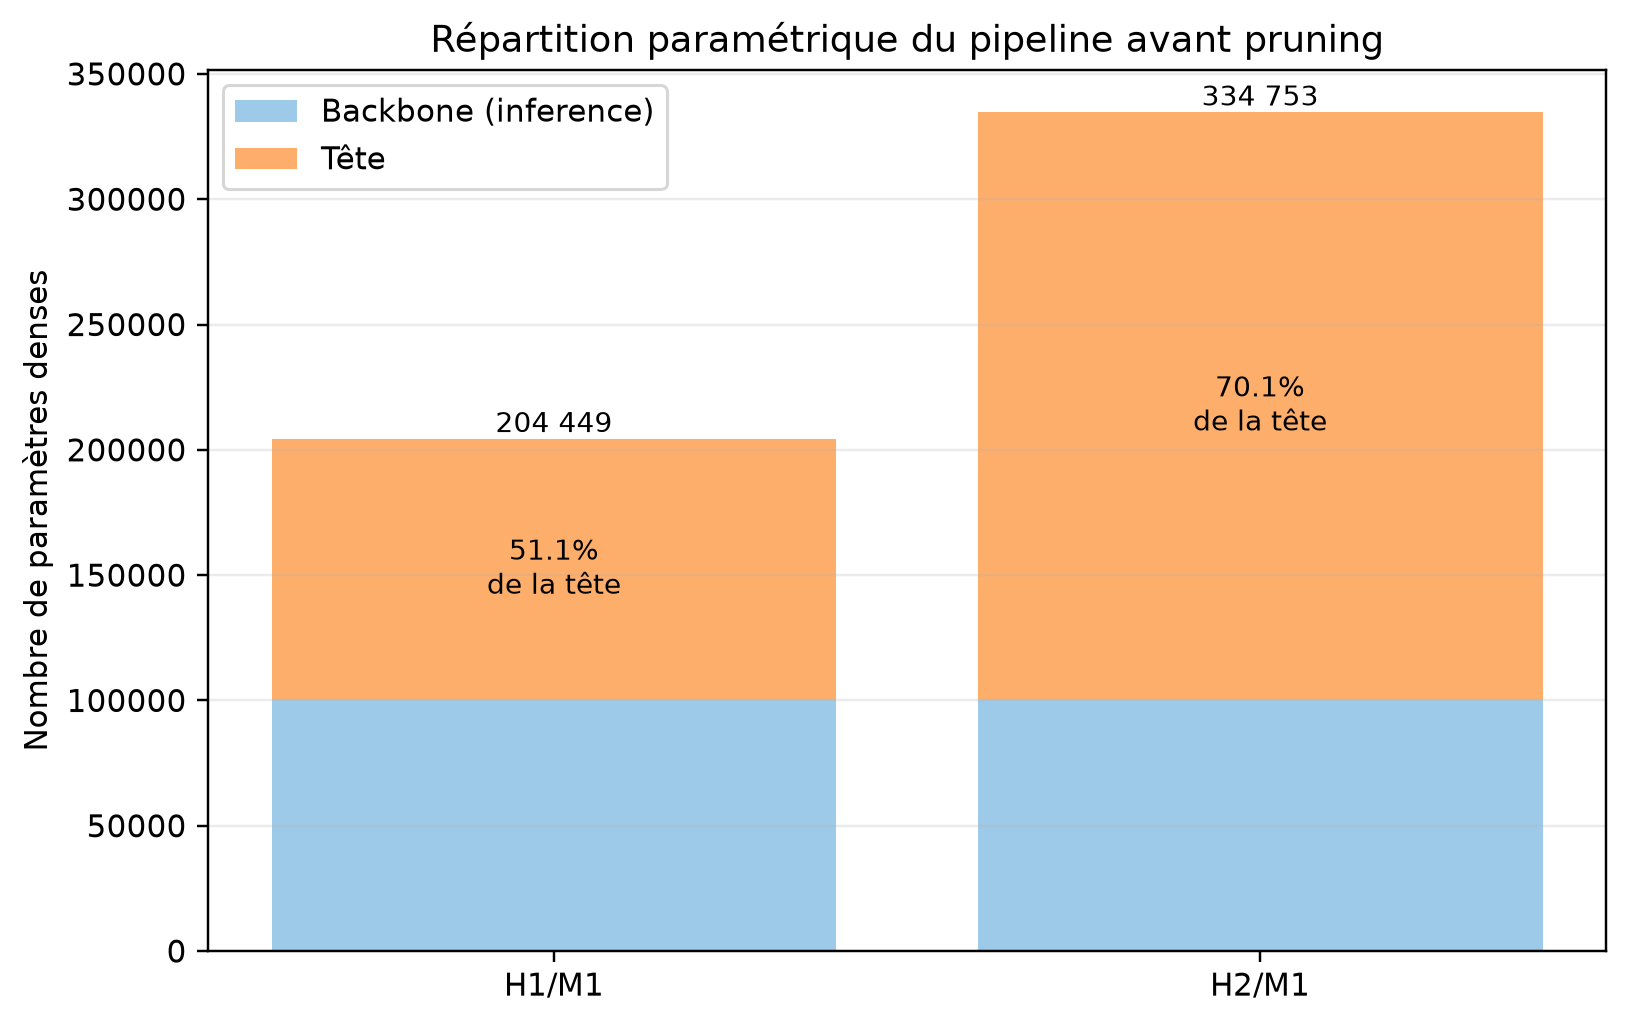
\includegraphics[width=0.82\textwidth]{../figures/theoriques/repartition_parametres_denses.png}
    \caption{Répartition des paramètres denses avant pruning. Le backbone ne
    compte ici que la table d'embeddings d'entrée nécessaire à l'inférence ; la
    table de sortie utilisée pour l'apprentissage CBOW est exclue. Le choix des
    nouvelles dimensions rend l'effet d'un pruning de la tête visible à
    l'échelle du pipeline complet.}
    \label{fig:resultats_repartition_parametres}
\end{figure}

La \autoref{fig:resultats_repartition_parametres} vérifie l'objectif recherché
par le changement d'hyperparamètres. Dans H1, le backbone et la tête ont des
tailles voisines ; dans H2, la tête contient plus de deux fois le nombre de
paramètres du backbone d'inférence. Une sparsification de H2 peut donc produire
un gain théorique sensible même lorsque W1 reste intact.

\begin{figure}[!htbp]
    \centering
    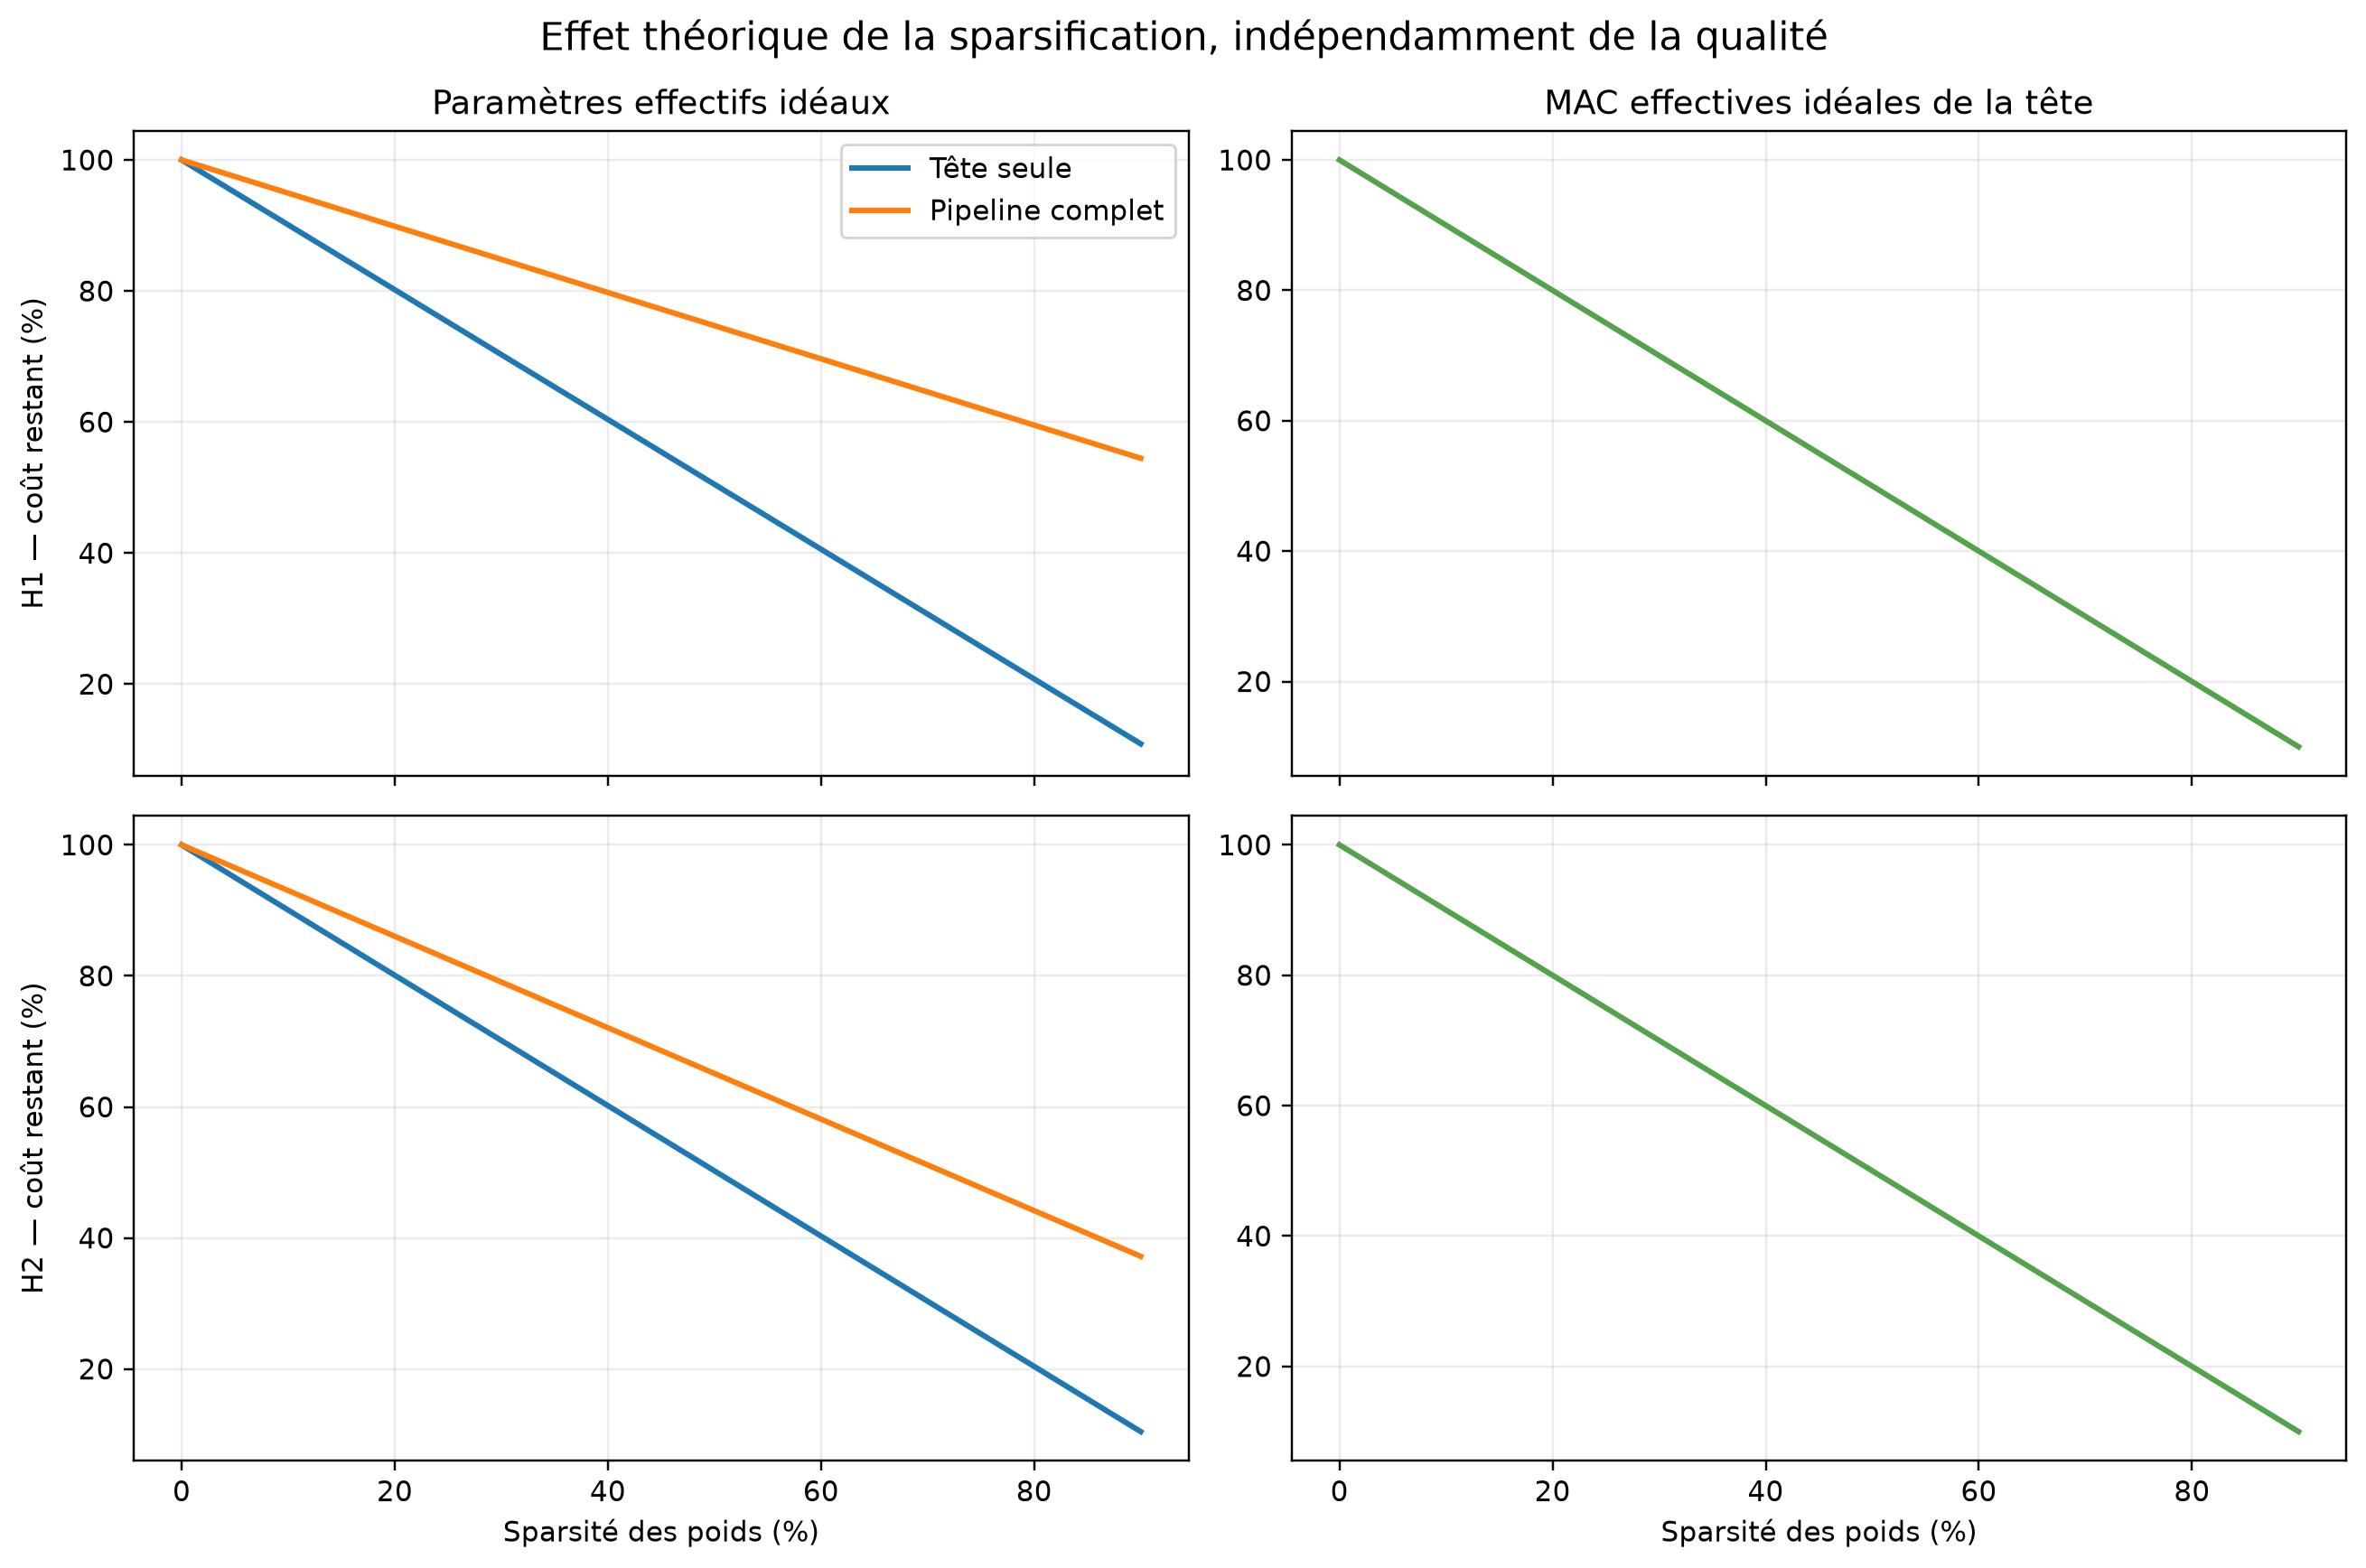
\includegraphics[width=0.94\textwidth]{../figures/theoriques/effet_theorique_sparsification.png}
    \caption{Effet théorique d'une sparsification croissante sur les paramètres
    et les MAC de la tête. Les coûts restants décroissent de façon affine avec
    la sparsité. Dans la vue des paramètres, la courbe du pipeline complet
    reste au-dessus de celle de la tête seule dès que la sparsité est non nulle,
    car elle inclut le coût fixe du backbone W1, qui n'est pas pruné. La
    réduction relative du pipeline est donc plus faible que celle de la tête.
    Ces courbes représentent un potentiel idéal, pas un gain matériel mesuré.}
    \label{fig:resultats_effet_theorique}
\end{figure}

À environ $50\,\%$ de sparsité, le nombre de paramètres effectifs de H1
passe de $104\,449$ à $52\,737$ et celui de H2 de $234\,753$ à environ
$118\,000$. En incluant W1, la réduction n'est plus de $50\,\%$, mais de
$25{,}3\,\%$ pour H1 et $34{,}9\,\%$ pour H2. Cette différence entre les deux
niveaux d'analyse justifie de les conserver dans toute la suite.

\subsection{Performances prédictives finales}
\label{ssec:resultats_tableau_principal}

Le \autoref{tab:resultats_principaux} rassemble les métriques du jeu de test.
Pour M2 et M3, la sparsité désigne la proportion de poids annulés dans la
tête. M4 est une architecture dense plus petite : sa sparsité interne vaut
donc zéro, même si son nombre de paramètres est voisin du nombre de paramètres
actifs des modèles prunés.

\begin{table}[!htbp]
    \centering
    \resizebox{\textwidth}{!}{%
    \begin{tabular}{|l|l|r|r|r|r|r|r|r|}
        \hline
        Tête & Modèle & Loss & Accuracy & F1 & ROC-AUC & Sparsité &
        $P_H^{\mathrm{eff}}$ & $P_{\mathrm{pipeline}}^{\mathrm{eff}}$ \\ \hline
        H1 & M1 & $0{,}5441$ & $72{,}92\,\%$ & $0{,}7397$ & $0{,}8009$ & $0\,\%$ & $104\,449$ & $204\,449$ \\ \hline
        H1 & M2 OBD & $0{,}5379$ & $73{,}20\,\%$ & $\mathbf{0{,}7561}$ & $0{,}8090$ & $50{,}00\,\%$ & $52\,737$ & $152\,737$ \\ \hline
        H1 & M3 OBD & $\mathbf{0{,}5353}$ & $\mathbf{73{,}57\,\%}$ & $0{,}7462$ & $\mathbf{0{,}8102}$ & $50{,}00\,\%$ & $52\,737$ & $152\,737$ \\ \hline
        H1 & M4 & $0{,}5449$ & $72{,}53\,\%$ & $0{,}7414$ & $0{,}7989$ & $0\,\%$ & $52\,225$ & $152\,225$ \\ \hline
        H2 & M1 & $\mathbf{0{,}5381}$ & $\mathbf{73{,}26\,\%}$ & $0{,}7393$ & $0{,}8038$ & $0\,\%$ & $234\,753$ & $334\,753$ \\ \hline
        H2 & M2 OBD & $0{,}5500$ & $72{,}07\,\%$ & $0{,}7441$ & $0{,}8027$ & $49{,}97\,\%$ & $118\,017$ & $218\,017$ \\ \hline
        H2 & M3 OBD & $0{,}5515$ & $73{,}02\,\%$ & $0{,}7435$ & $\mathbf{0{,}8048}$ & $49{,}97\,\%$ & $118\,017$ & $218\,017$ \\ \hline
        H2 & M4 & $0{,}5419$ & $72{,}92\,\%$ & $0{,}7449$ & $0{,}8029$ & $0\,\%$ & $117\,505$ & $217\,505$ \\ \hline
        H2 & MINT-M2 & $0{,}6787$ & $53{,}02\,\%$ & $0{,}2192$ & $0{,}7336$ & $49{,}95\,\%$ & $118\,063$ & $218\,063$ \\ \hline
        H2 & MINT-M3 & $0{,}5409$ & $72{,}68\,\%$ & $\mathbf{0{,}7505}$ & $0{,}8046$ & $49{,}95\,\%$ & $118\,063$ & $218\,063$ \\ \hline
    \end{tabular}}
    \caption{Résultats du run final sur les $3\,276$ textes de test. Les
    valeurs en gras indiquent le meilleur résultat de chaque tête et de chaque
    métrique ; elles ne constituent pas un test de significativité statistique.}
    \label{tab:resultats_principaux}
\end{table}

Pour H1, le pruning OBD ne dégrade pas la qualité : M2 obtient même le meilleur
F1 de la tête, $0{,}7561$, soit $+0{,}0165$ par rapport à M1. M3 présente la
meilleure loss, la meilleure accuracy et la meilleure ROC-AUC de H1, mais son
F1 est inférieur à celui de M2. Le réentraînement n'améliore donc pas toutes
les métriques simultanément. M4 reste proche de M1, ce qui indique qu'une tête
plus petite pouvait ici être entraînée directement sans perte importante.

L'absence de première place pour H1/M1 n'est pas paradoxale : une capacité plus
élevée ne garantit pas une meilleure généralisation. Surtout, ce classement ne
peut pas être attribué au seul pruning. OBD comporte six tours de trois
époques : M2 a déjà reçu 15 époques supplémentaires à partir du checkpoint M1,
et M3 en cumule 18. Comme M1 est sélectionné selon la loss de validation et que
le run n'utilise qu'une graine, le tableau montre que la compression préserve
la qualité, mais pas qu'elle améliore H1. Plusieurs graines et un protocole
d'entraînement strictement identique seraient nécessaires pour isoler cet effet.

Pour H2, les trois solutions de taille réduite après entraînement --- OBD-M2,
OBD-M3 et M4 --- atteignent des F1 compris entre $0{,}7435$ et $0{,}7449$. Le
meilleur F1 de H2 est obtenu par MINT-M3 avec $0{,}7505$, soit $+0{,}0112$ par
rapport à M1. Ce résultat doit toutefois être lu avec MINT-M2 : l'application
du masque seule fait chuter le F1 à $0{,}2192$. Sa précision reste élevée
($0{,}8963$), mais son rappel tombe à $0{,}1249$ ; le modèle prédit donc très
peu d'exemples positifs. Le réentraînement contraint est indispensable pour
recalibrer les activations et récupérer la performance.

\subsection{Convergence et comportement de la loss}
\label{ssec:resultats_convergence}

\begin{figure}[!htbp]
    \centering
    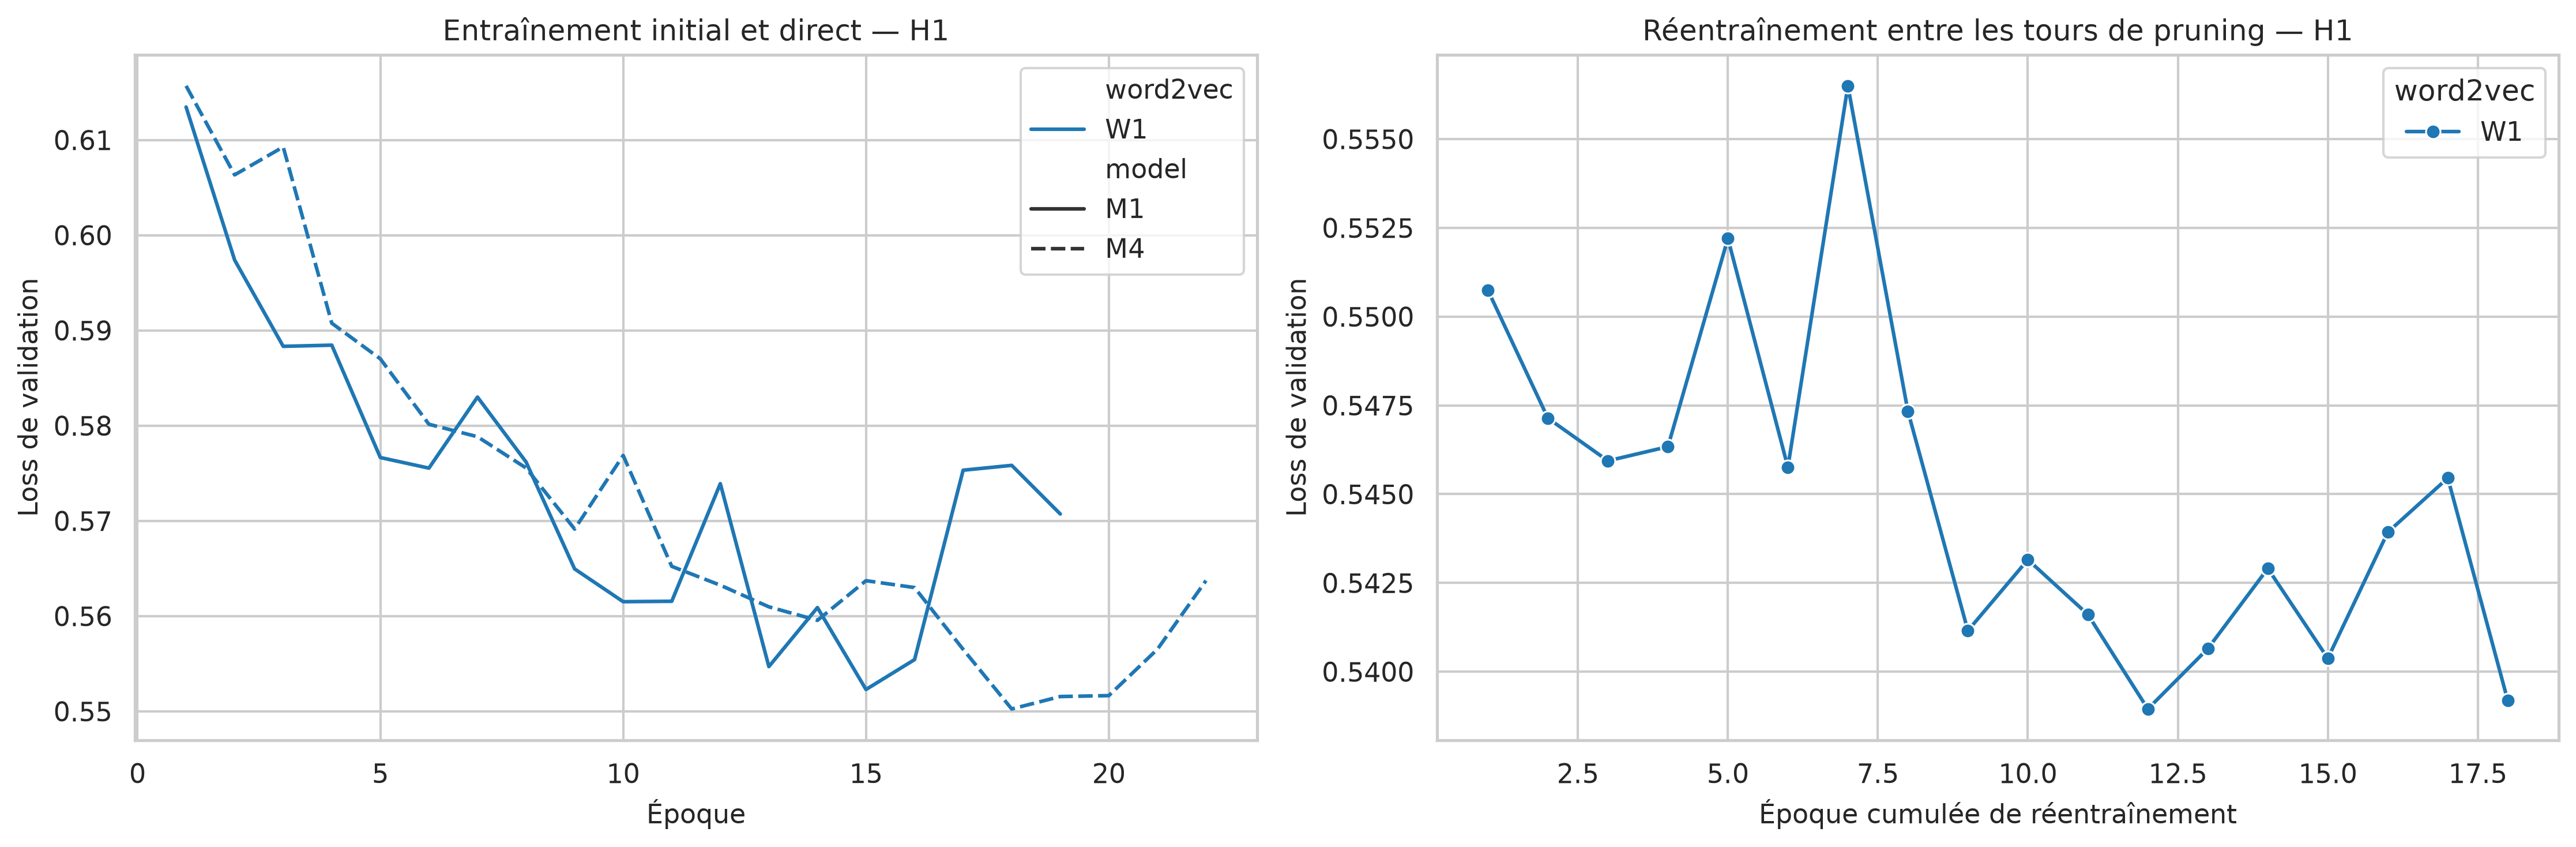
\includegraphics[width=0.94\textwidth]{../figures/experimentales/training_losses_H1.png}
    \par\smallskip\small (a) Tête H1.\par\medskip
    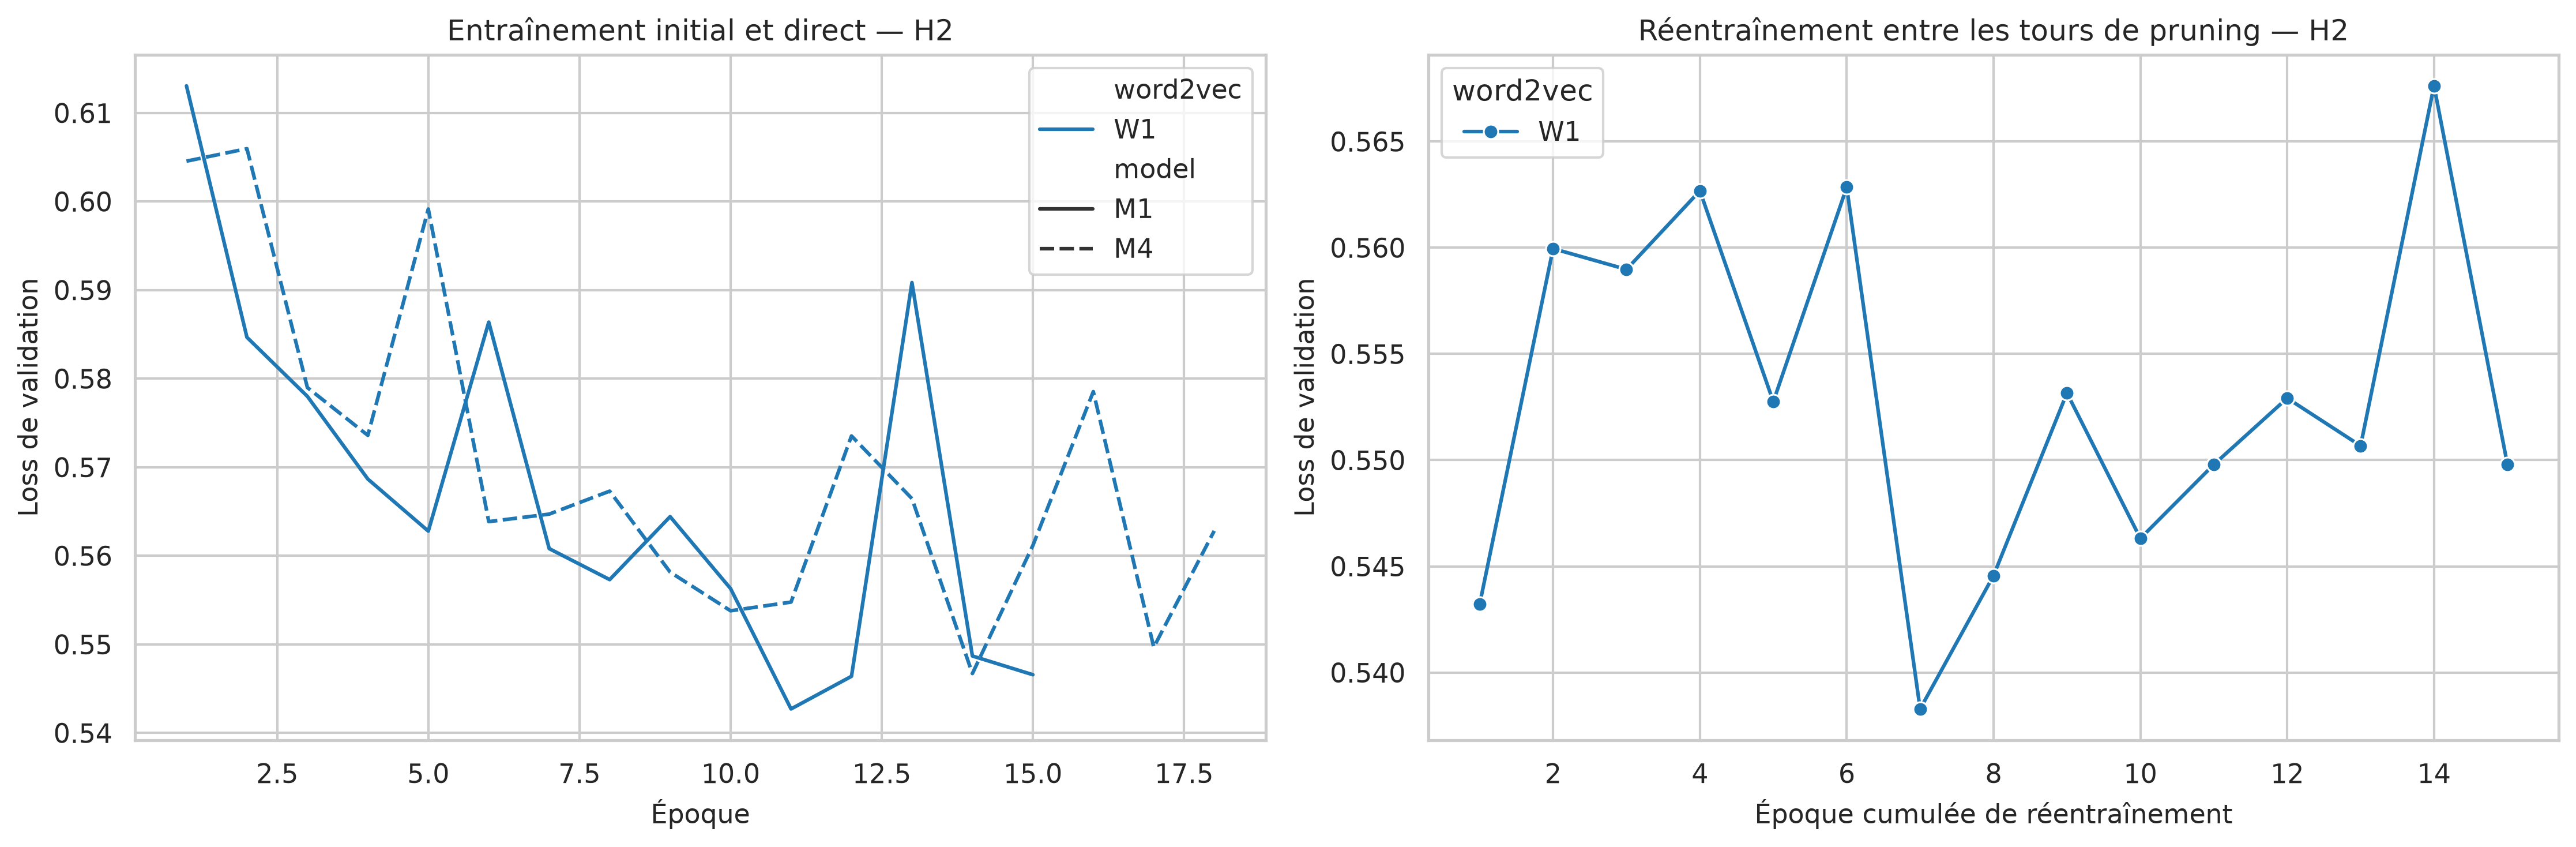
\includegraphics[width=0.94\textwidth]{../figures/experimentales/training_losses_H2.png}
    \par\smallskip\small (b) Tête H2.
    \caption{Loss de validation pendant l'entraînement dense de M1 et M4
    (graphiques de gauche) et pendant les réentraînements successifs d'OBD
    (graphiques de droite). L'abscisse des graphiques de droite concatène les
    trois époques de chaque tour de pruning.}
    \label{fig:resultats_training_losses}
\end{figure}

L'arrêt anticipé conserve l'époque de plus faible loss de validation. H1/M1
s'arrête après 19 époques et restaure l'époque 15
($\mathcal{L}_{\mathrm{val}}=0{,}5523$), tandis que H2/M1 s'arrête après 15
époques et restaure l'époque 11 ($0{,}5427$). Les oscillations visibles en
fin d'entraînement justifient ce mécanisme : la loss d'entraînement continue
de diminuer alors que la loss de validation ne s'améliore plus de manière
monotone. Les phases courtes de réentraînement OBD produisent elles aussi des
variations non monotones, ce qui explique qu'une amélioration de la loss ne se
traduise pas systématiquement par une hausse du F1 au seuil de décision $0{,}5$.

\subsection{Trajectoires du pruning OBD}
\label{ssec:resultats_obd}

\begin{figure}[!htbp]
    \centering
    \begin{minipage}[t]{0.49\textwidth}
        \centering
        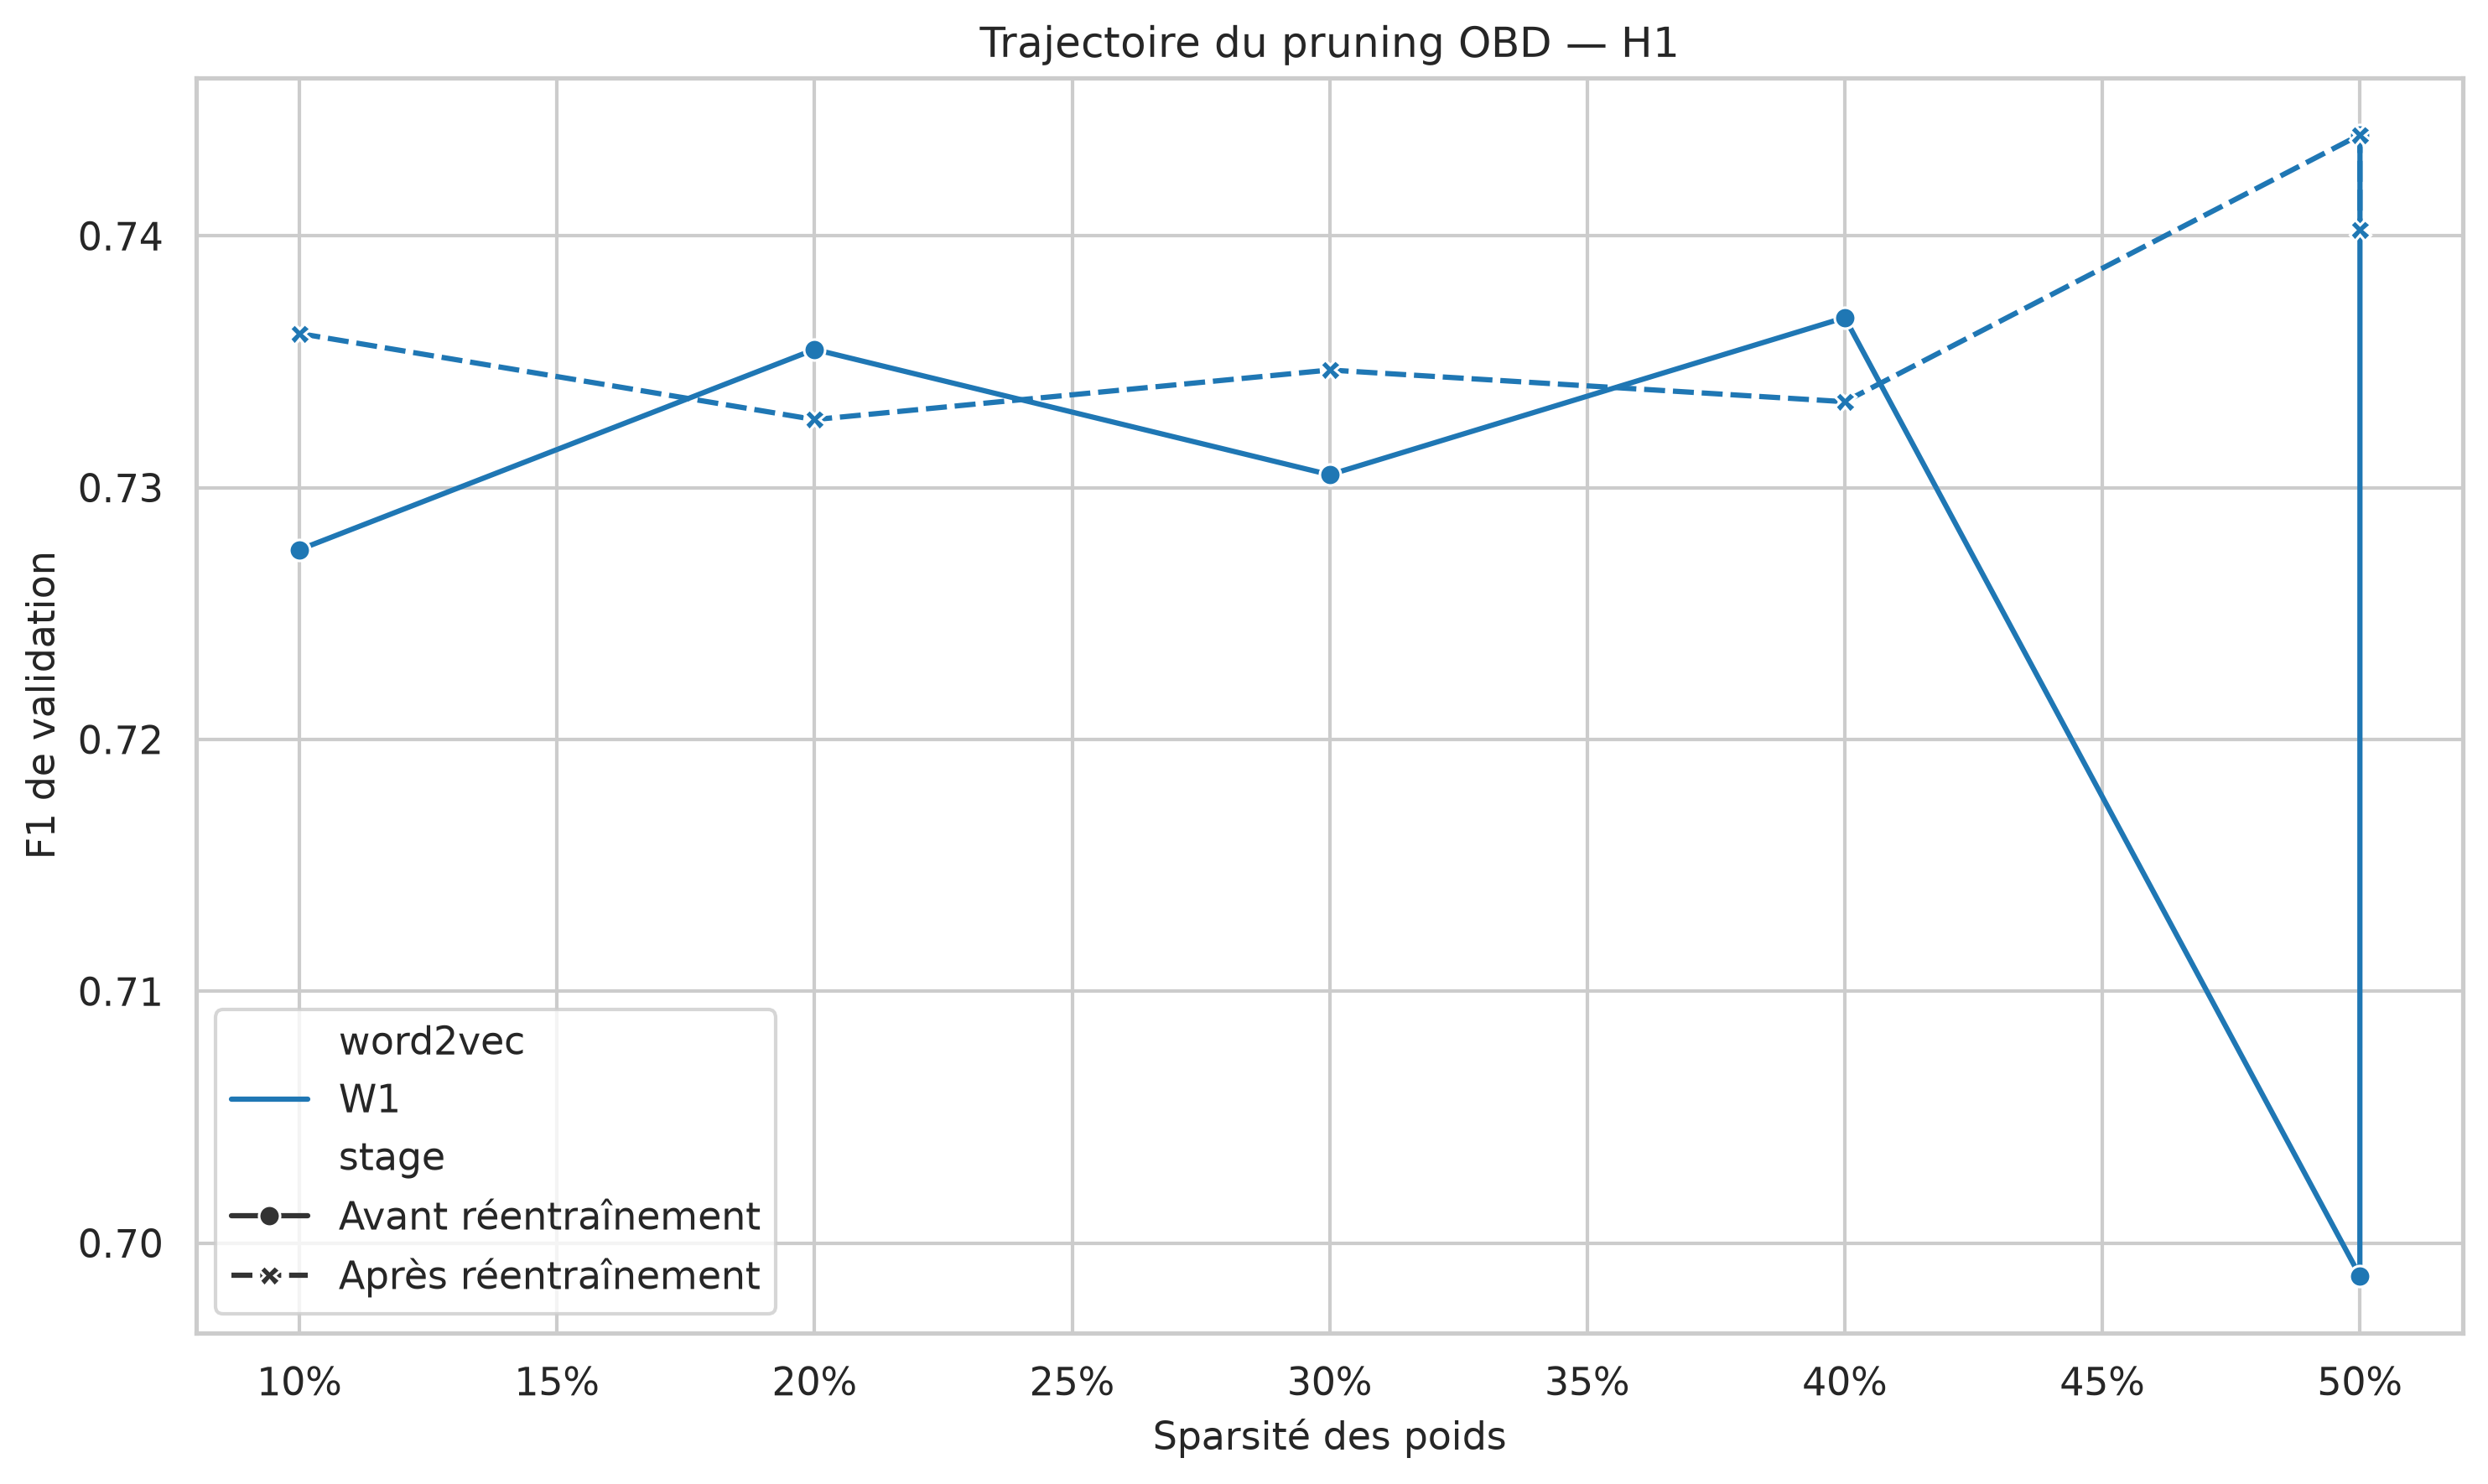
\includegraphics[width=\linewidth]{../figures/experimentales/pruning_trajectory_H1.png}
        \small (a) H1.
    \end{minipage}
    \hfill
    \begin{minipage}[t]{0.49\textwidth}
        \centering
        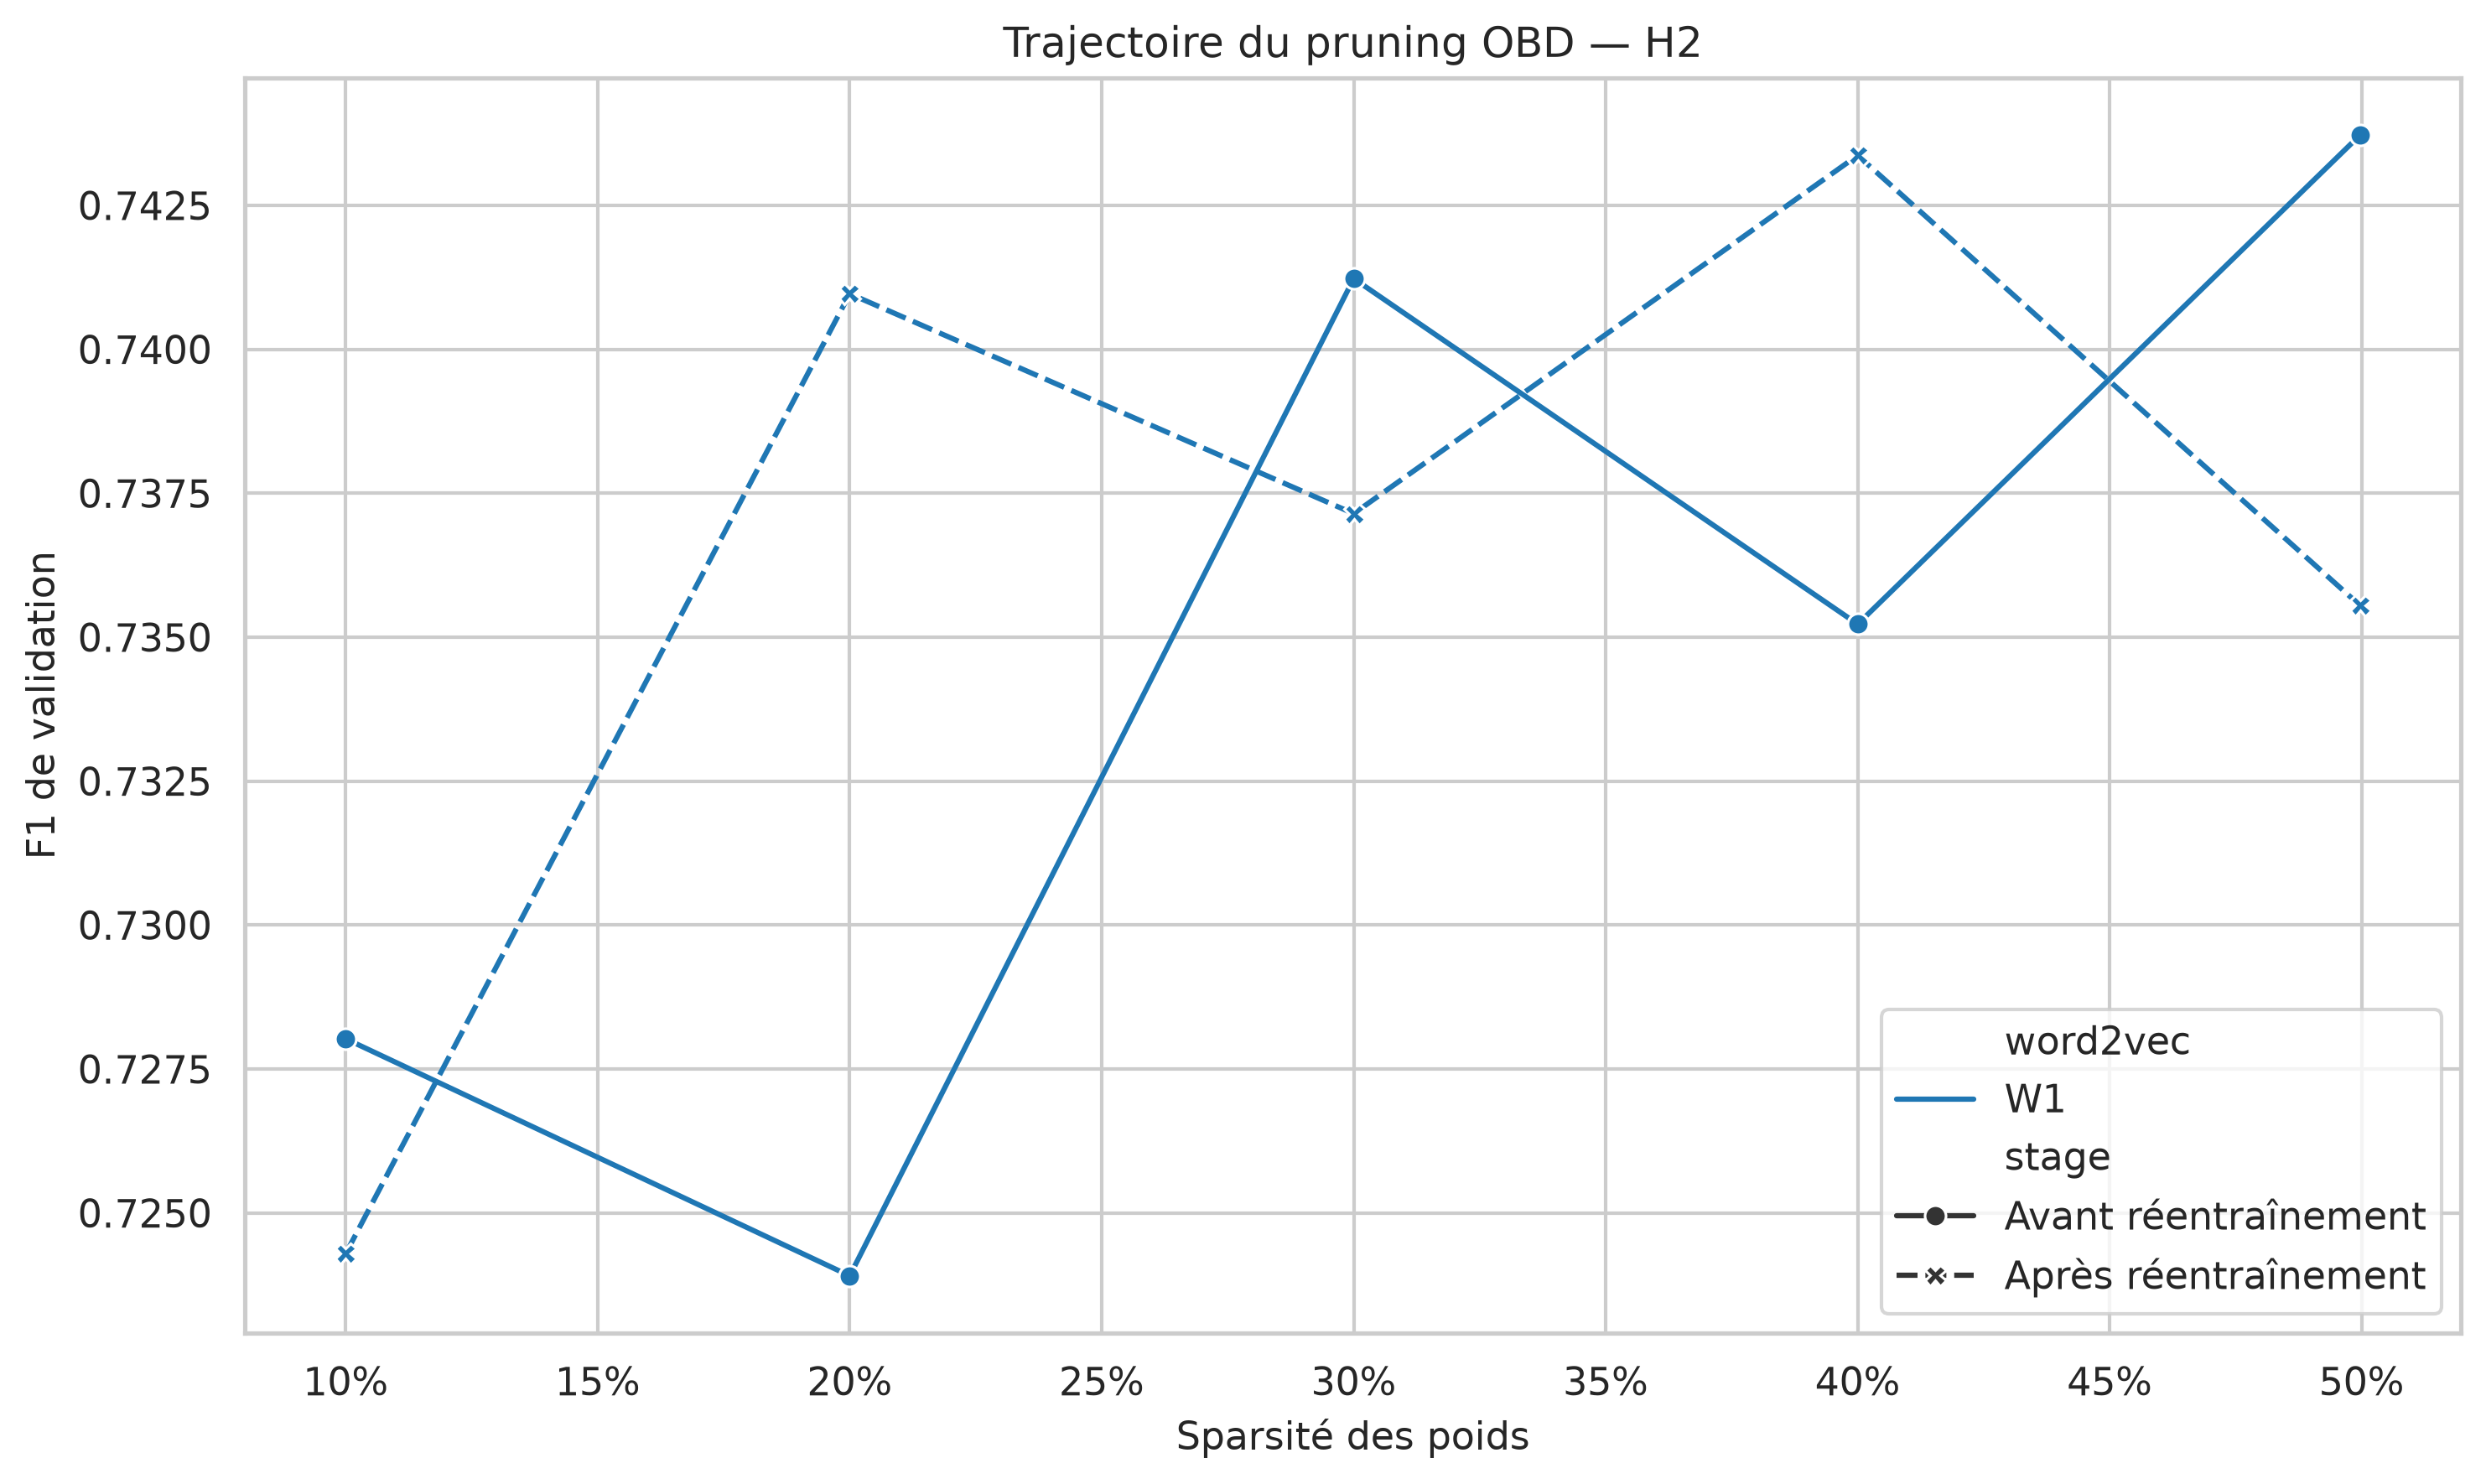
\includegraphics[width=\linewidth]{../figures/experimentales/pruning_trajectory_H2.png}
        \small (b) H2.
    \end{minipage}
    \caption{F1 de validation avant et après chaque réentraînement OBD. Les
    scores sont recalculés après chaque tour. Pour H1, un dernier micro-tour
    permet d'atteindre exactement $50\,\%$ après les arrondis en nombres entiers
    de poids.}
    \label{fig:resultats_trajectoires_obd}
\end{figure}

La trajectoire de H1 reste stable jusqu'à $40\,\%$ de sparsité. Au voisinage
de $50\,\%$, le F1 de validation passe de $0{,}6987$ juste après le cinquième
pruning à $0{,}7440$ après réentraînement : la phase de cicatrisation est ici
déterminante. H2 est moins régulier. Son F1 final vaut $0{,}7437$ avant le
dernier réentraînement et $0{,}7355$ après. Le modèle restauré minimise la
loss parmi les trois nouvelles époques, mais cette règle ne garantit ni de
surpasser l'état avant réentraînement ni de maximiser le F1. OBD préserve donc
globalement la qualité à $50\,\%$, sans rendre chaque tour individuellement
bénéfique.

\subsection{Comportement spécifique de MINT}
\label{ssec:resultats_mint}

\begin{figure}[!htbp]
    \centering
    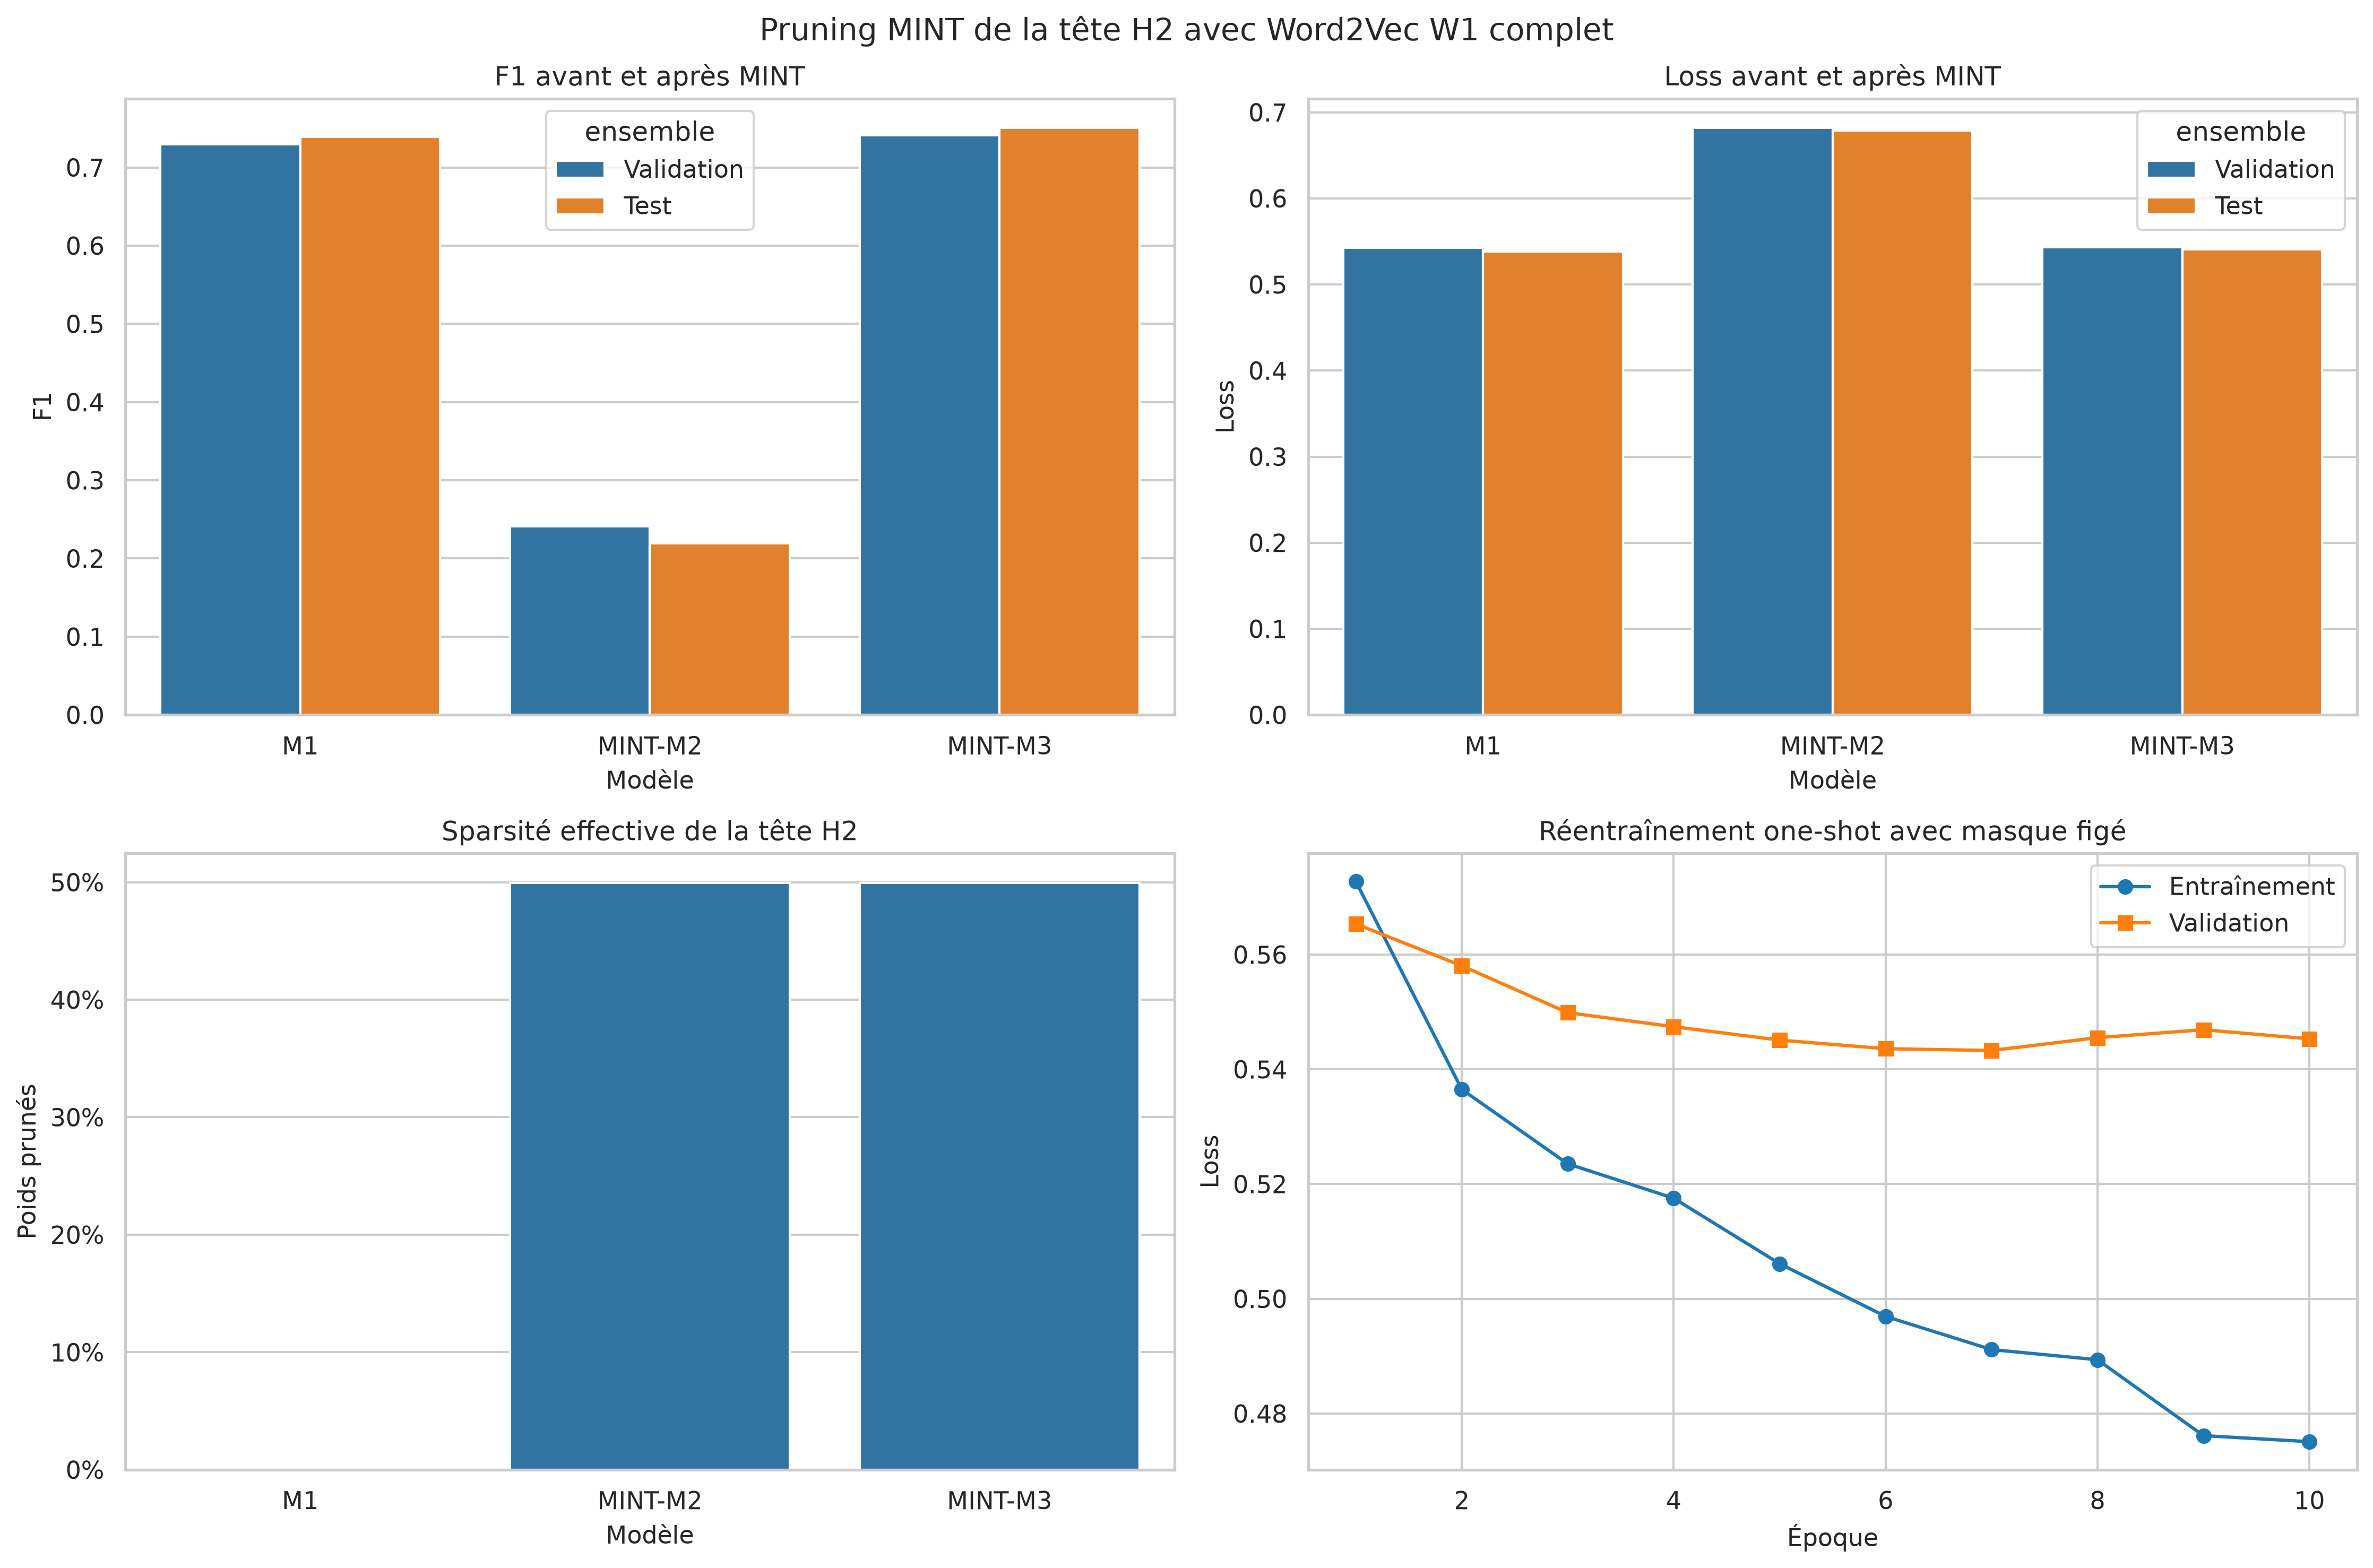
\includegraphics[width=0.94\textwidth]{../figures/experimentales/mint_summary_W1_H2.png}
    \caption{Synthèse de MINT sur H2 : F1, loss, sparsité et courbes du
    réentraînement one-shot. MINT-M2 est le modèle immédiatement masqué ;
    MINT-M3 utilise exactement le même masque après dix époques de
    réentraînement contraint.}
    \label{fig:resultats_mint_resume}
\end{figure}

La \autoref{fig:resultats_mint_resume} montre que le masque MINT modifie
fortement l'échelle des activations avant adaptation des poids restants. Le F1
et la loss de MINT-M2 se dégradent simultanément, puis MINT-M3 retrouve une loss
de test de $0{,}5409$, proche de celle de M1 ($0{,}5381$), et dépasse son F1.
La loss de validation du réentraînement atteint son minimum à l'époque 7 ;
les trois dernières époques ne l'améliorent plus. L'état restauré est donc
bien antérieur à la dernière mise à jour affichée.

\begin{figure}[!htbp]
    \centering
    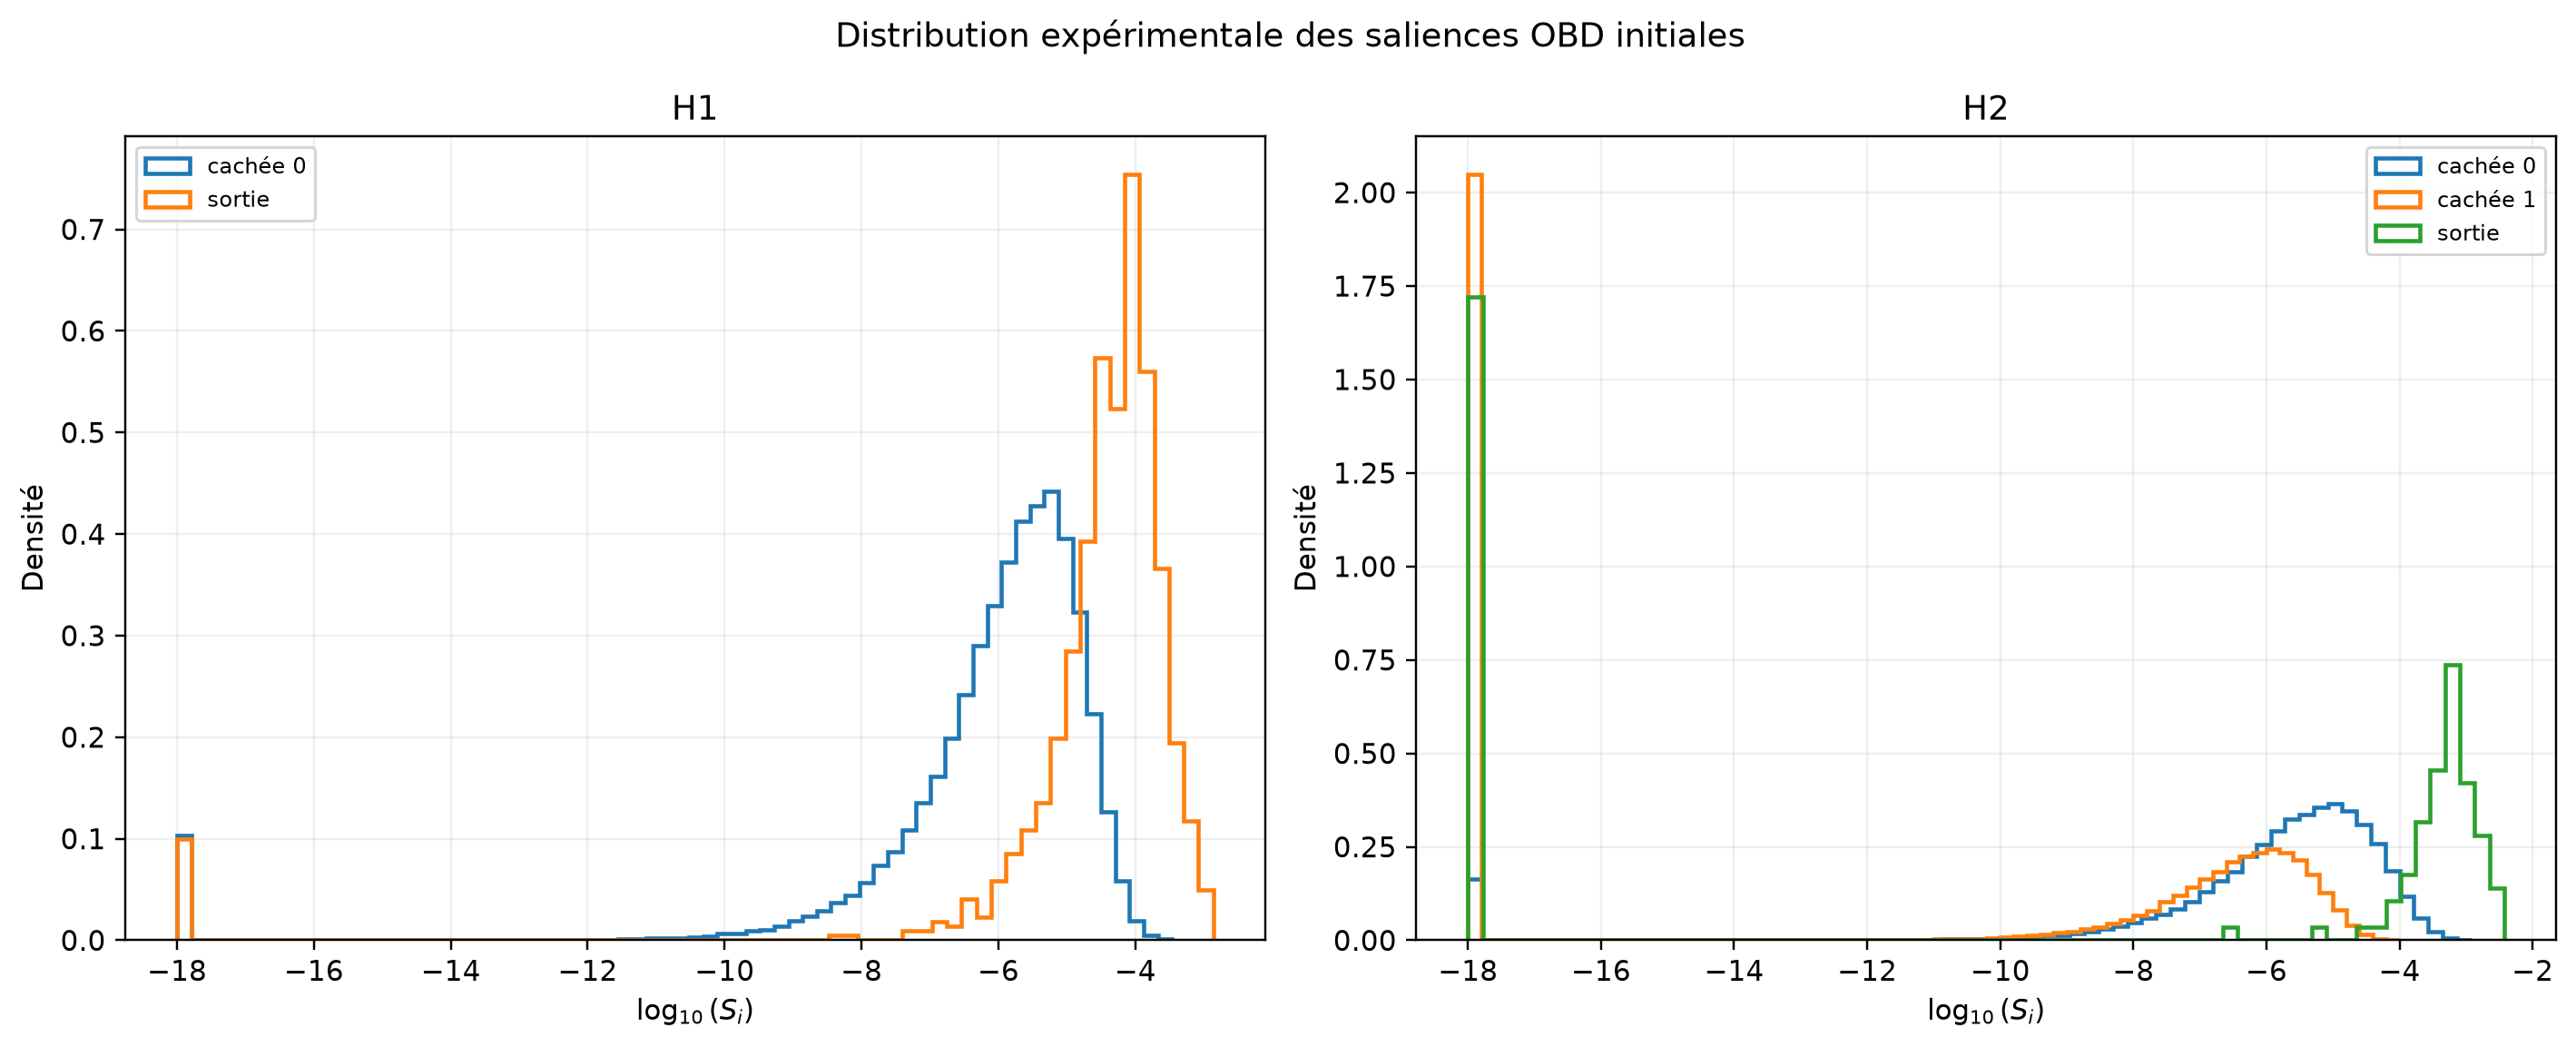
\includegraphics[width=0.94\textwidth]{../figures/experimentales/distribution_scores_obd.png}
    \par\smallskip\small (a) Saliences OBD initiales en échelle logarithmique.\par\medskip
    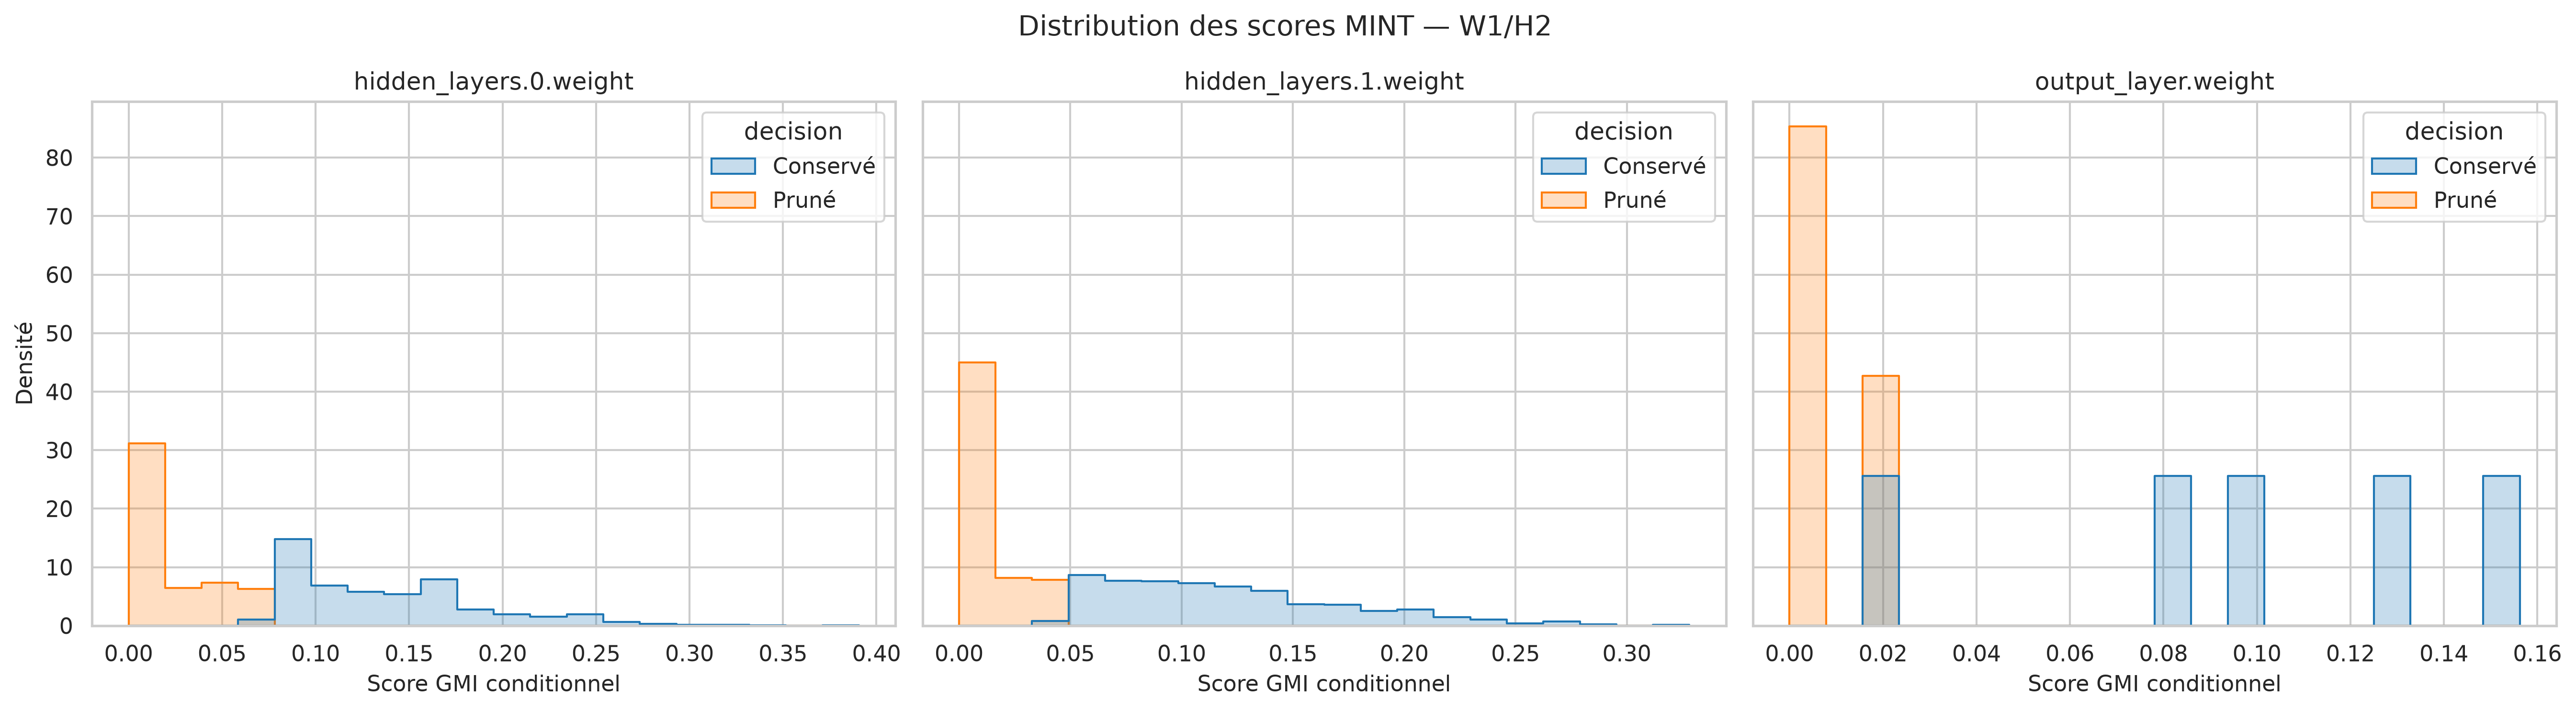
\includegraphics[width=0.98\textwidth]{../figures/experimentales/mint_score_distributions_W1_H2.png}
    \par\smallskip\small (b) Scores MINT conservés et prunés par couche.
    \caption{Distributions des scores propres aux deux méthodes. Leurs
    échelles et leurs significations diffèrent : OBD approxime une hausse
    locale de loss par poids, tandis que MINT mesure une dépendance
    conditionnelle par bloc. Une comparaison verticale directe de leurs
    valeurs brutes serait donc incorrecte.}
    \label{fig:resultats_distributions_scores}
\end{figure}

Les saliences OBD s'étendent sur de nombreux ordres de grandeur. Cette forte
asymétrie fournit une population importante de poids de très faible salience,
ce qui est cohérent avec la bonne tenue du modèle pendant les premiers tours.
Les scores MINT sont plus discrets, car l'estimateur dépend du nombre entier
d'arêtes croisées parmi $m=64$ observations. Les blocs prunés ont, par
construction, des scores plus faibles que les blocs conservés. La dernière
couche n'annule que $37{,}5\,\%$ de ses poids contre environ $50\,\%$ dans les
deux couches cachées, car elle ne contient que huit blocs et le nombre de blocs
supprimés doit être entier.

\subsection{ROC et effet du seuil de décision}
\label{ssec:resultats_roc}

\begin{figure}[!htbp]
    \centering
    \begin{minipage}[t]{0.48\textwidth}
        \centering
        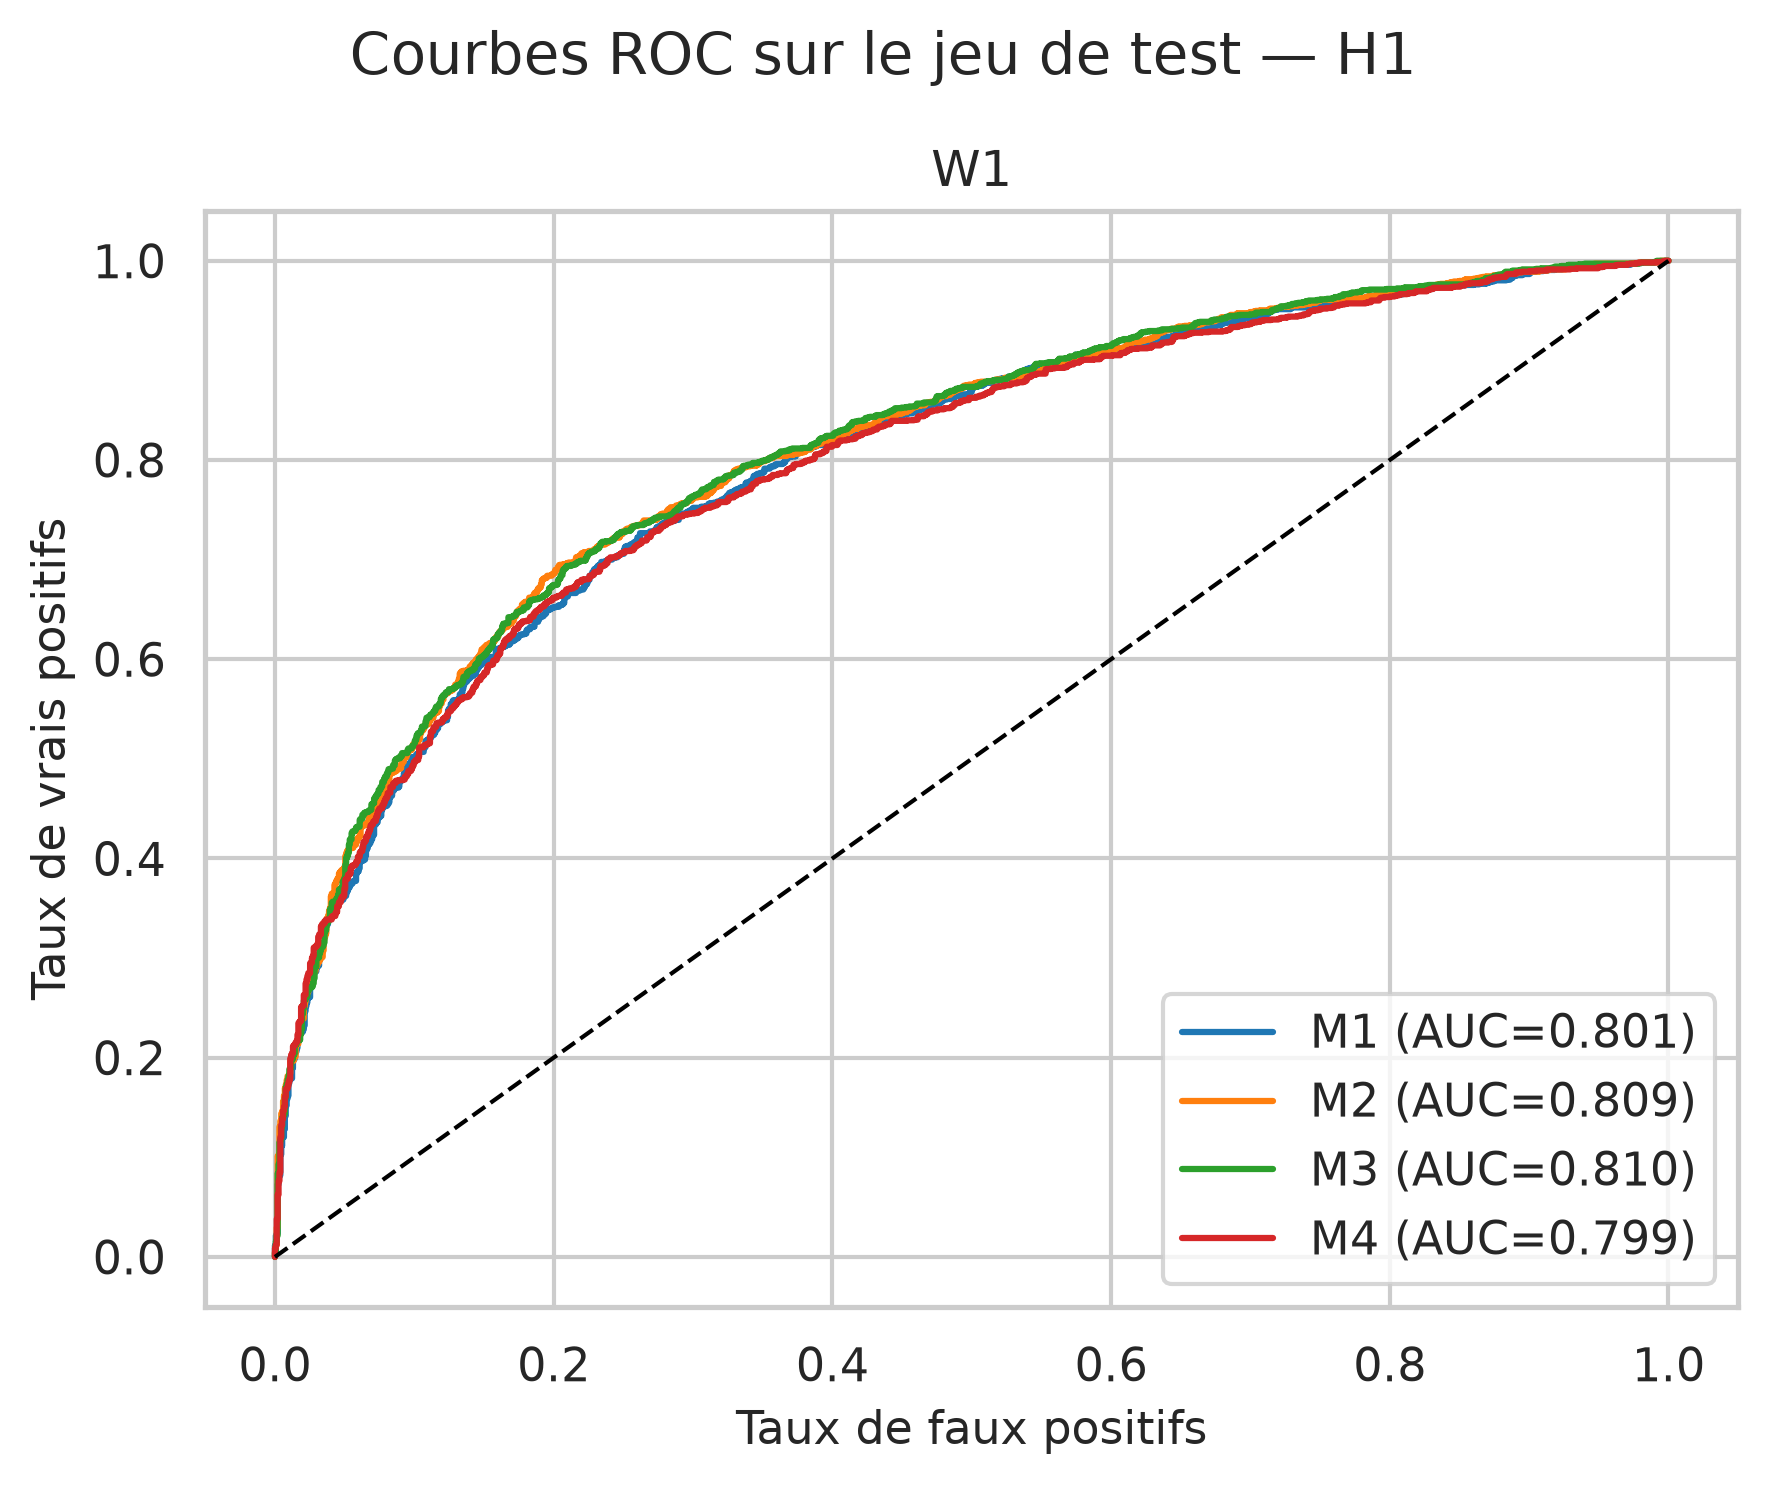
\includegraphics[width=\linewidth]{../figures/experimentales/roc_curves_H1.png}
        \small (a) H1.
    \end{minipage}
    \hfill
    \begin{minipage}[t]{0.48\textwidth}
        \centering
        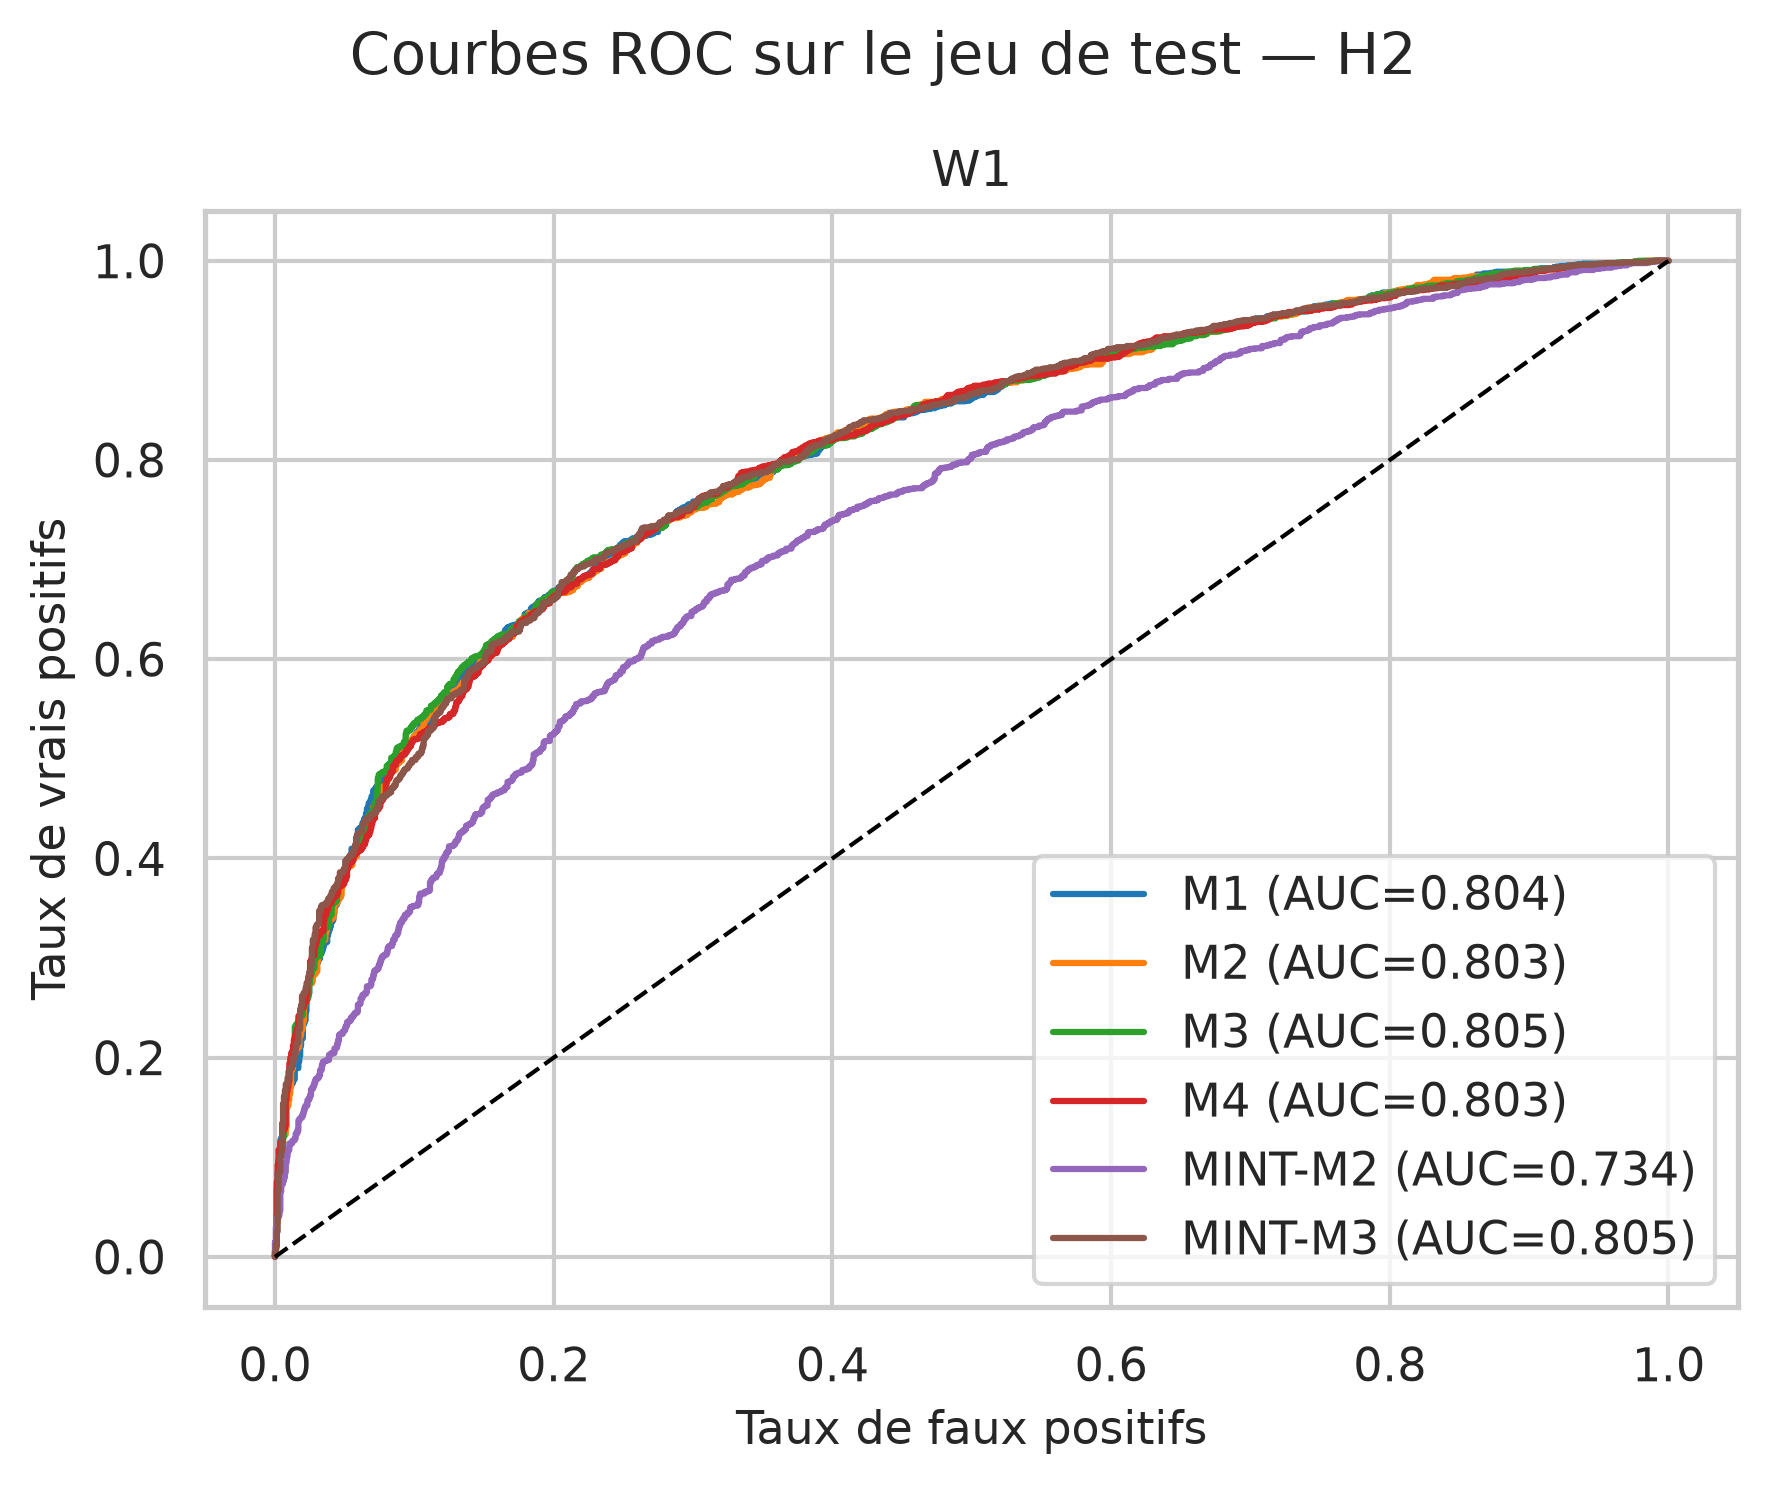
\includegraphics[width=\linewidth]{../figures/experimentales/roc_curves_H2.png}
        \small (b) H2, avec les variantes MINT.
    \end{minipage}
    \caption{Courbes ROC sur le jeu de test. L'aire sous la courbe mesure le
    classement des exemples sur tous les seuils, contrairement au F1 et à
    l'accuracy calculés au seuil fixe $0{,}5$.}
    \label{fig:resultats_roc}
\end{figure}

Les variantes finales de H1 ont des ROC-AUC comprises entre $0{,}7989$ et
$0{,}8102$, et celles de H2 entre $0{,}8027$ et $0{,}8048$. Les courbes sont
donc proches malgré les différences de F1. MINT-M2 constitue l'exception : son
ROC-AUC de $0{,}7336$ reste supérieure au hasard alors que son F1 vaut seulement
$0{,}2192$. Une partie de son effondrement provient ainsi du seuil et de la
calibration, mais la baisse d'AUC montre qu'il perd aussi une capacité de
classement. MINT-M3 restaure les deux aspects.

\subsection{Compromis qualité--mémoire et qualité--calcul}
\label{ssec:resultats_pareto}

\begin{figure}[!htbp]
    \centering
    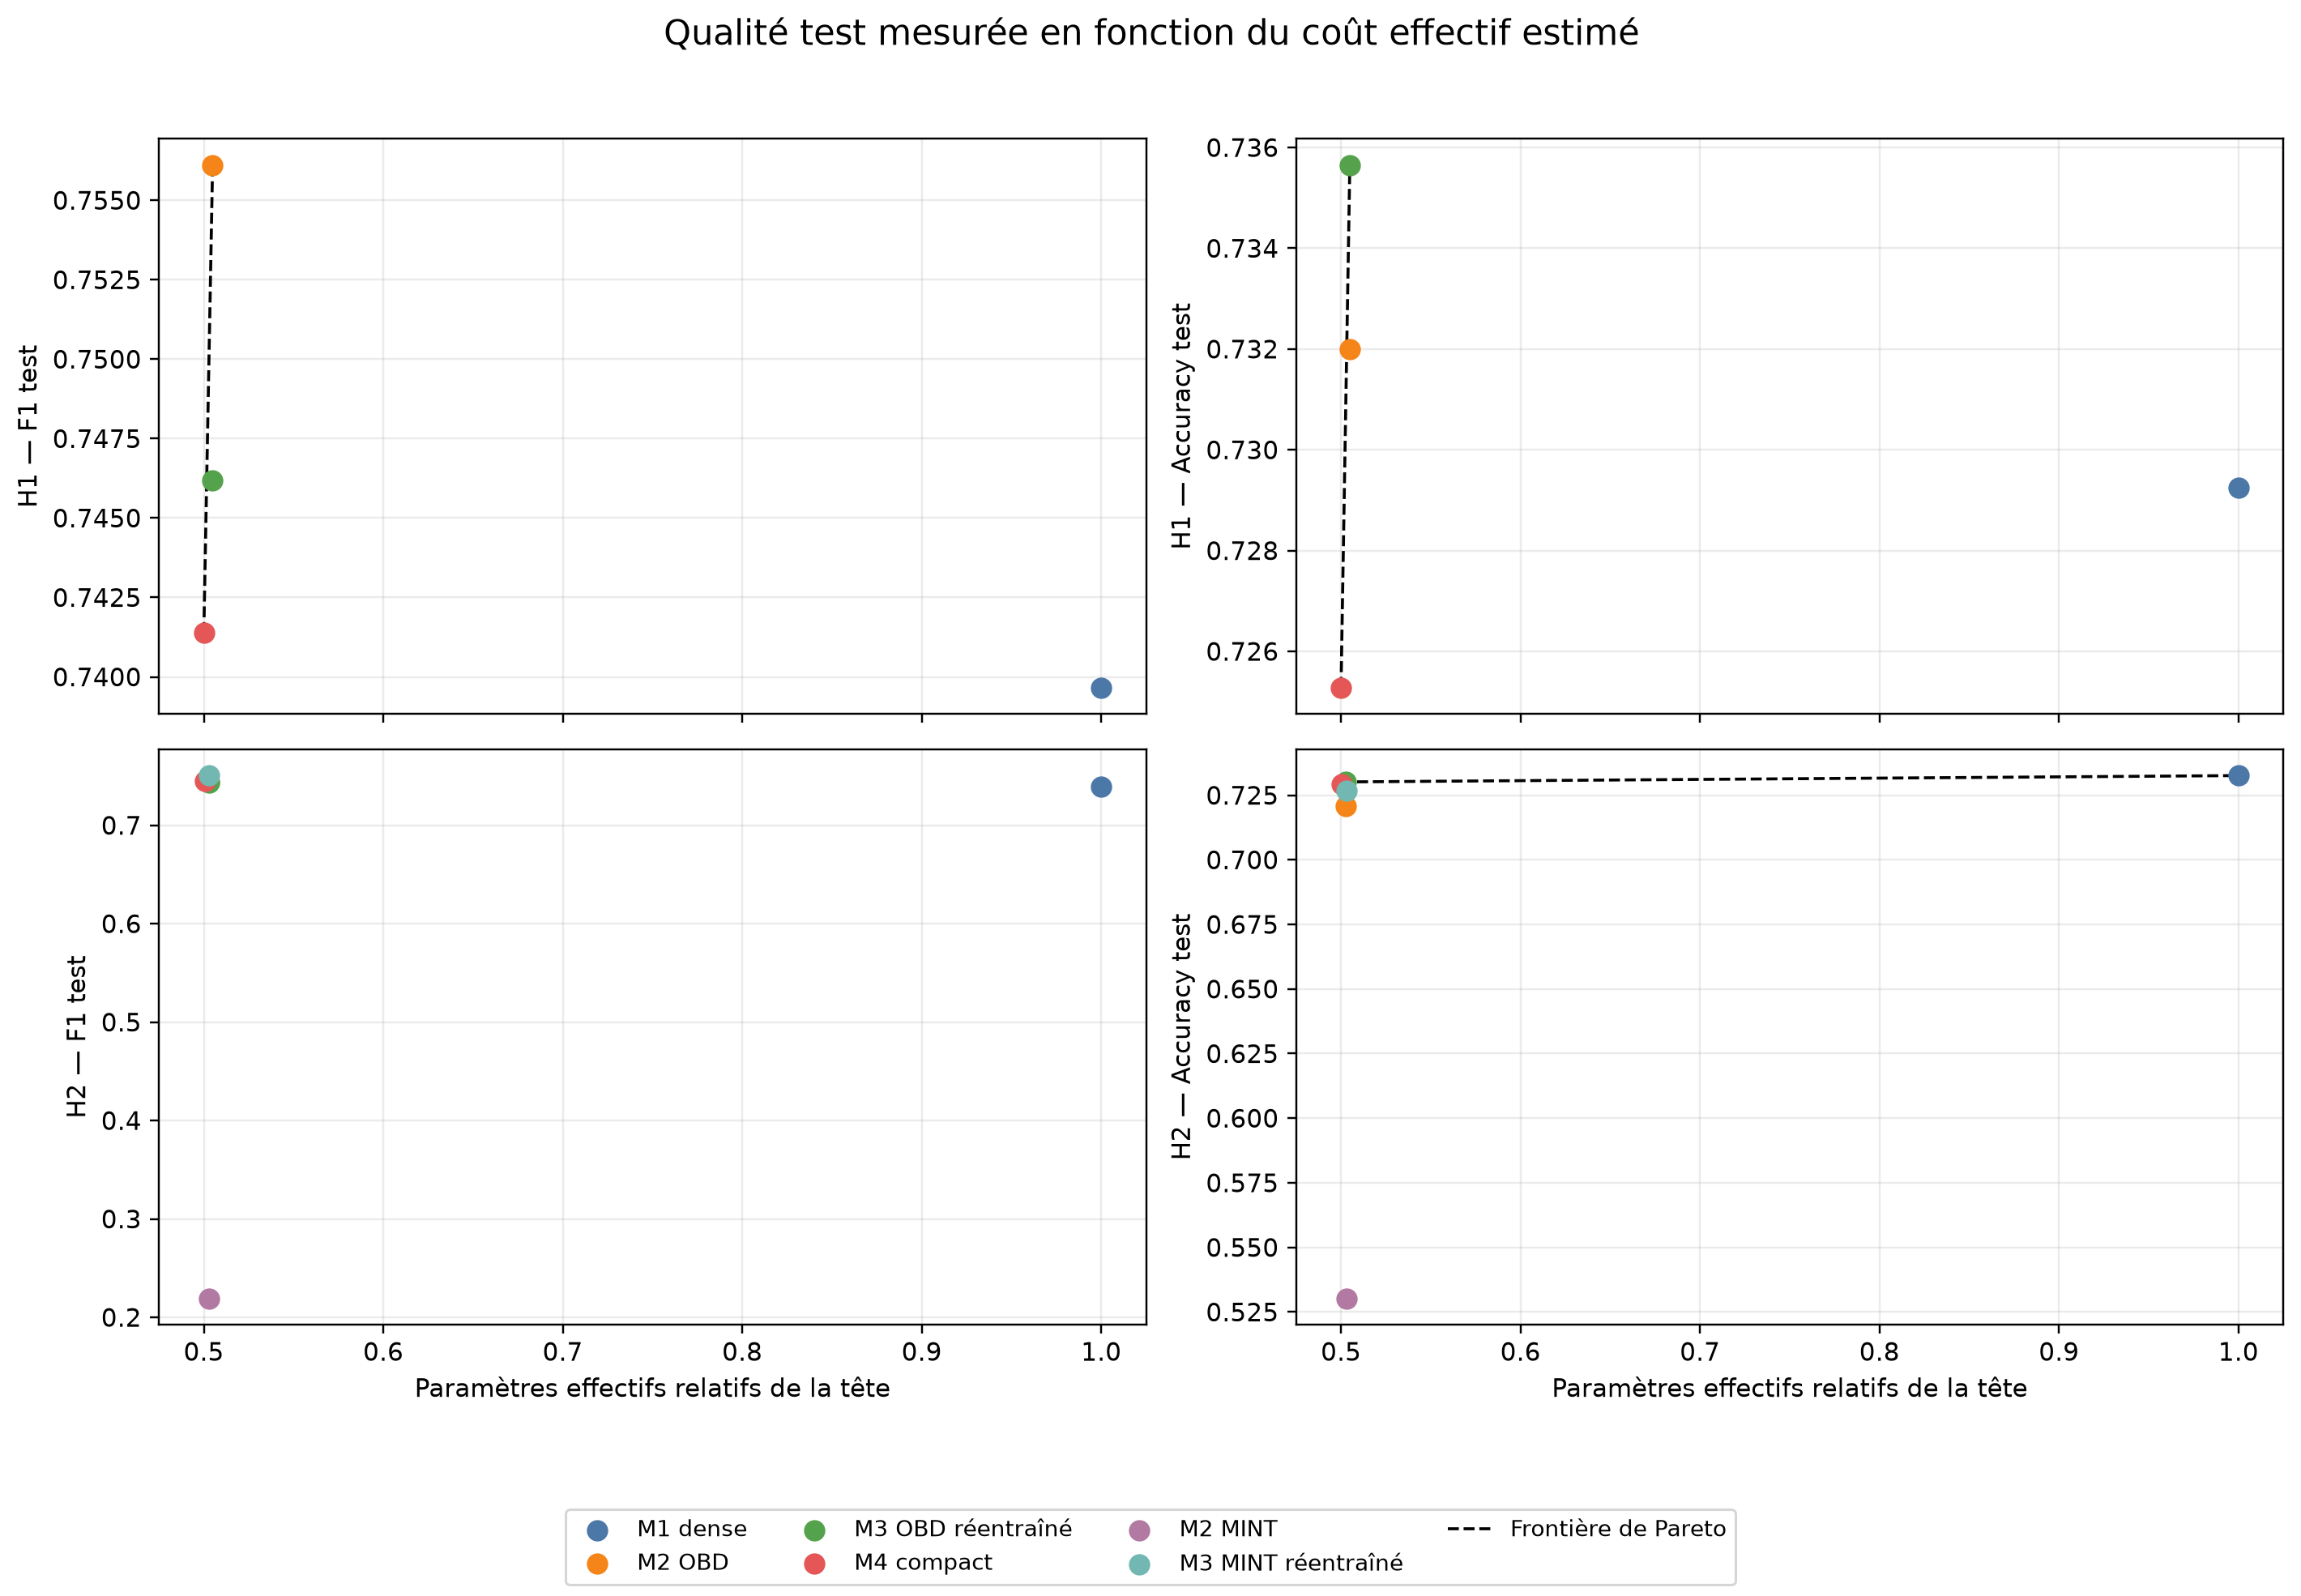
\includegraphics[width=0.96\textwidth]{../figures/experimentales/qualite_memoire_tete_pareto.png}
    \caption{F1 et accuracy de test en fonction des paramètres effectifs de
    la tête, normalisés par M1. Les pointillés relient les solutions non
    dominées. M4 est compté avec ses dimensions physiques réduites ; M2 et M3
    sont comptés selon leur nombre idéal de poids actifs.}
    \label{fig:resultats_pareto_memoire_tete}
\end{figure}

\begin{figure}[!htbp]
    \centering
    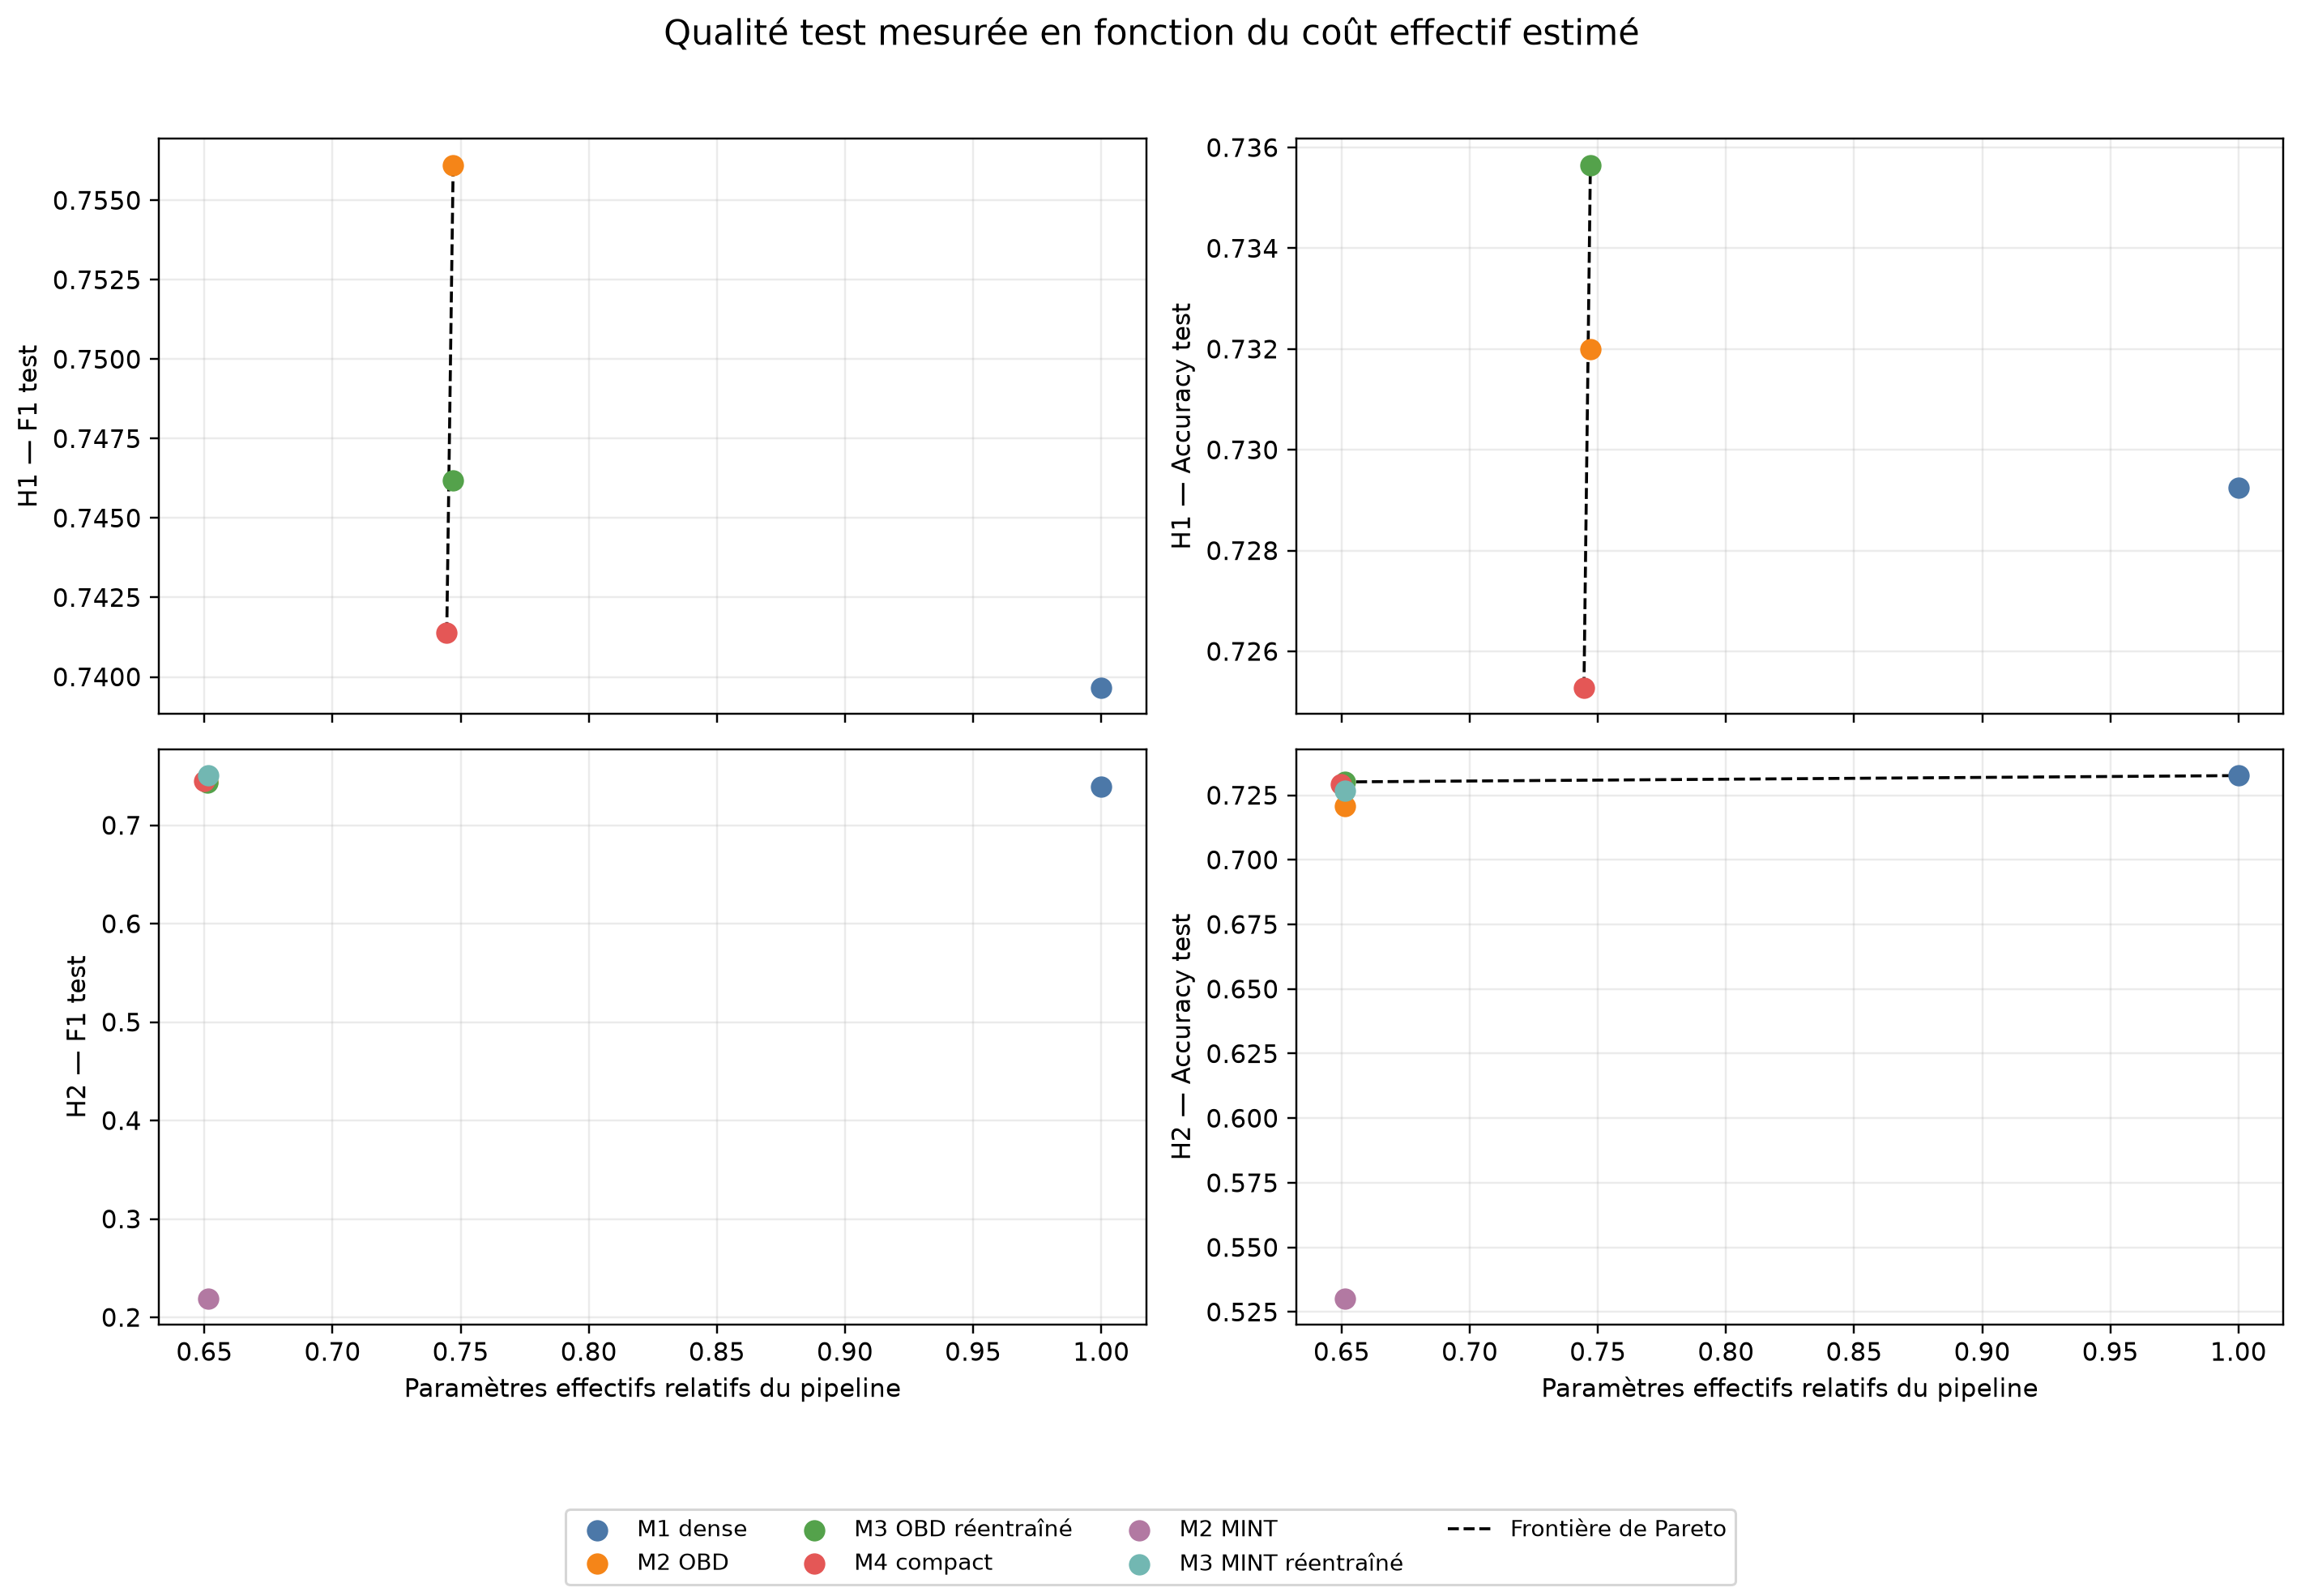
\includegraphics[width=0.96\textwidth]{../figures/experimentales/qualite_memoire_pipeline_pareto.png}
    \caption{Même compromis en incluant les $100\,000$ paramètres fixes de
    W1. Les modèles H1 compressés conservent environ $74{,}5\,\%$ du coût de
    M1 ; les modèles H2 compressés en conservent environ $65\,\%$. MINT-M2 est
    dominé en raison de sa forte perte de qualité.}
    \label{fig:resultats_pareto_memoire_pipeline}
\end{figure}

\begin{figure}[!htbp]
    \centering
    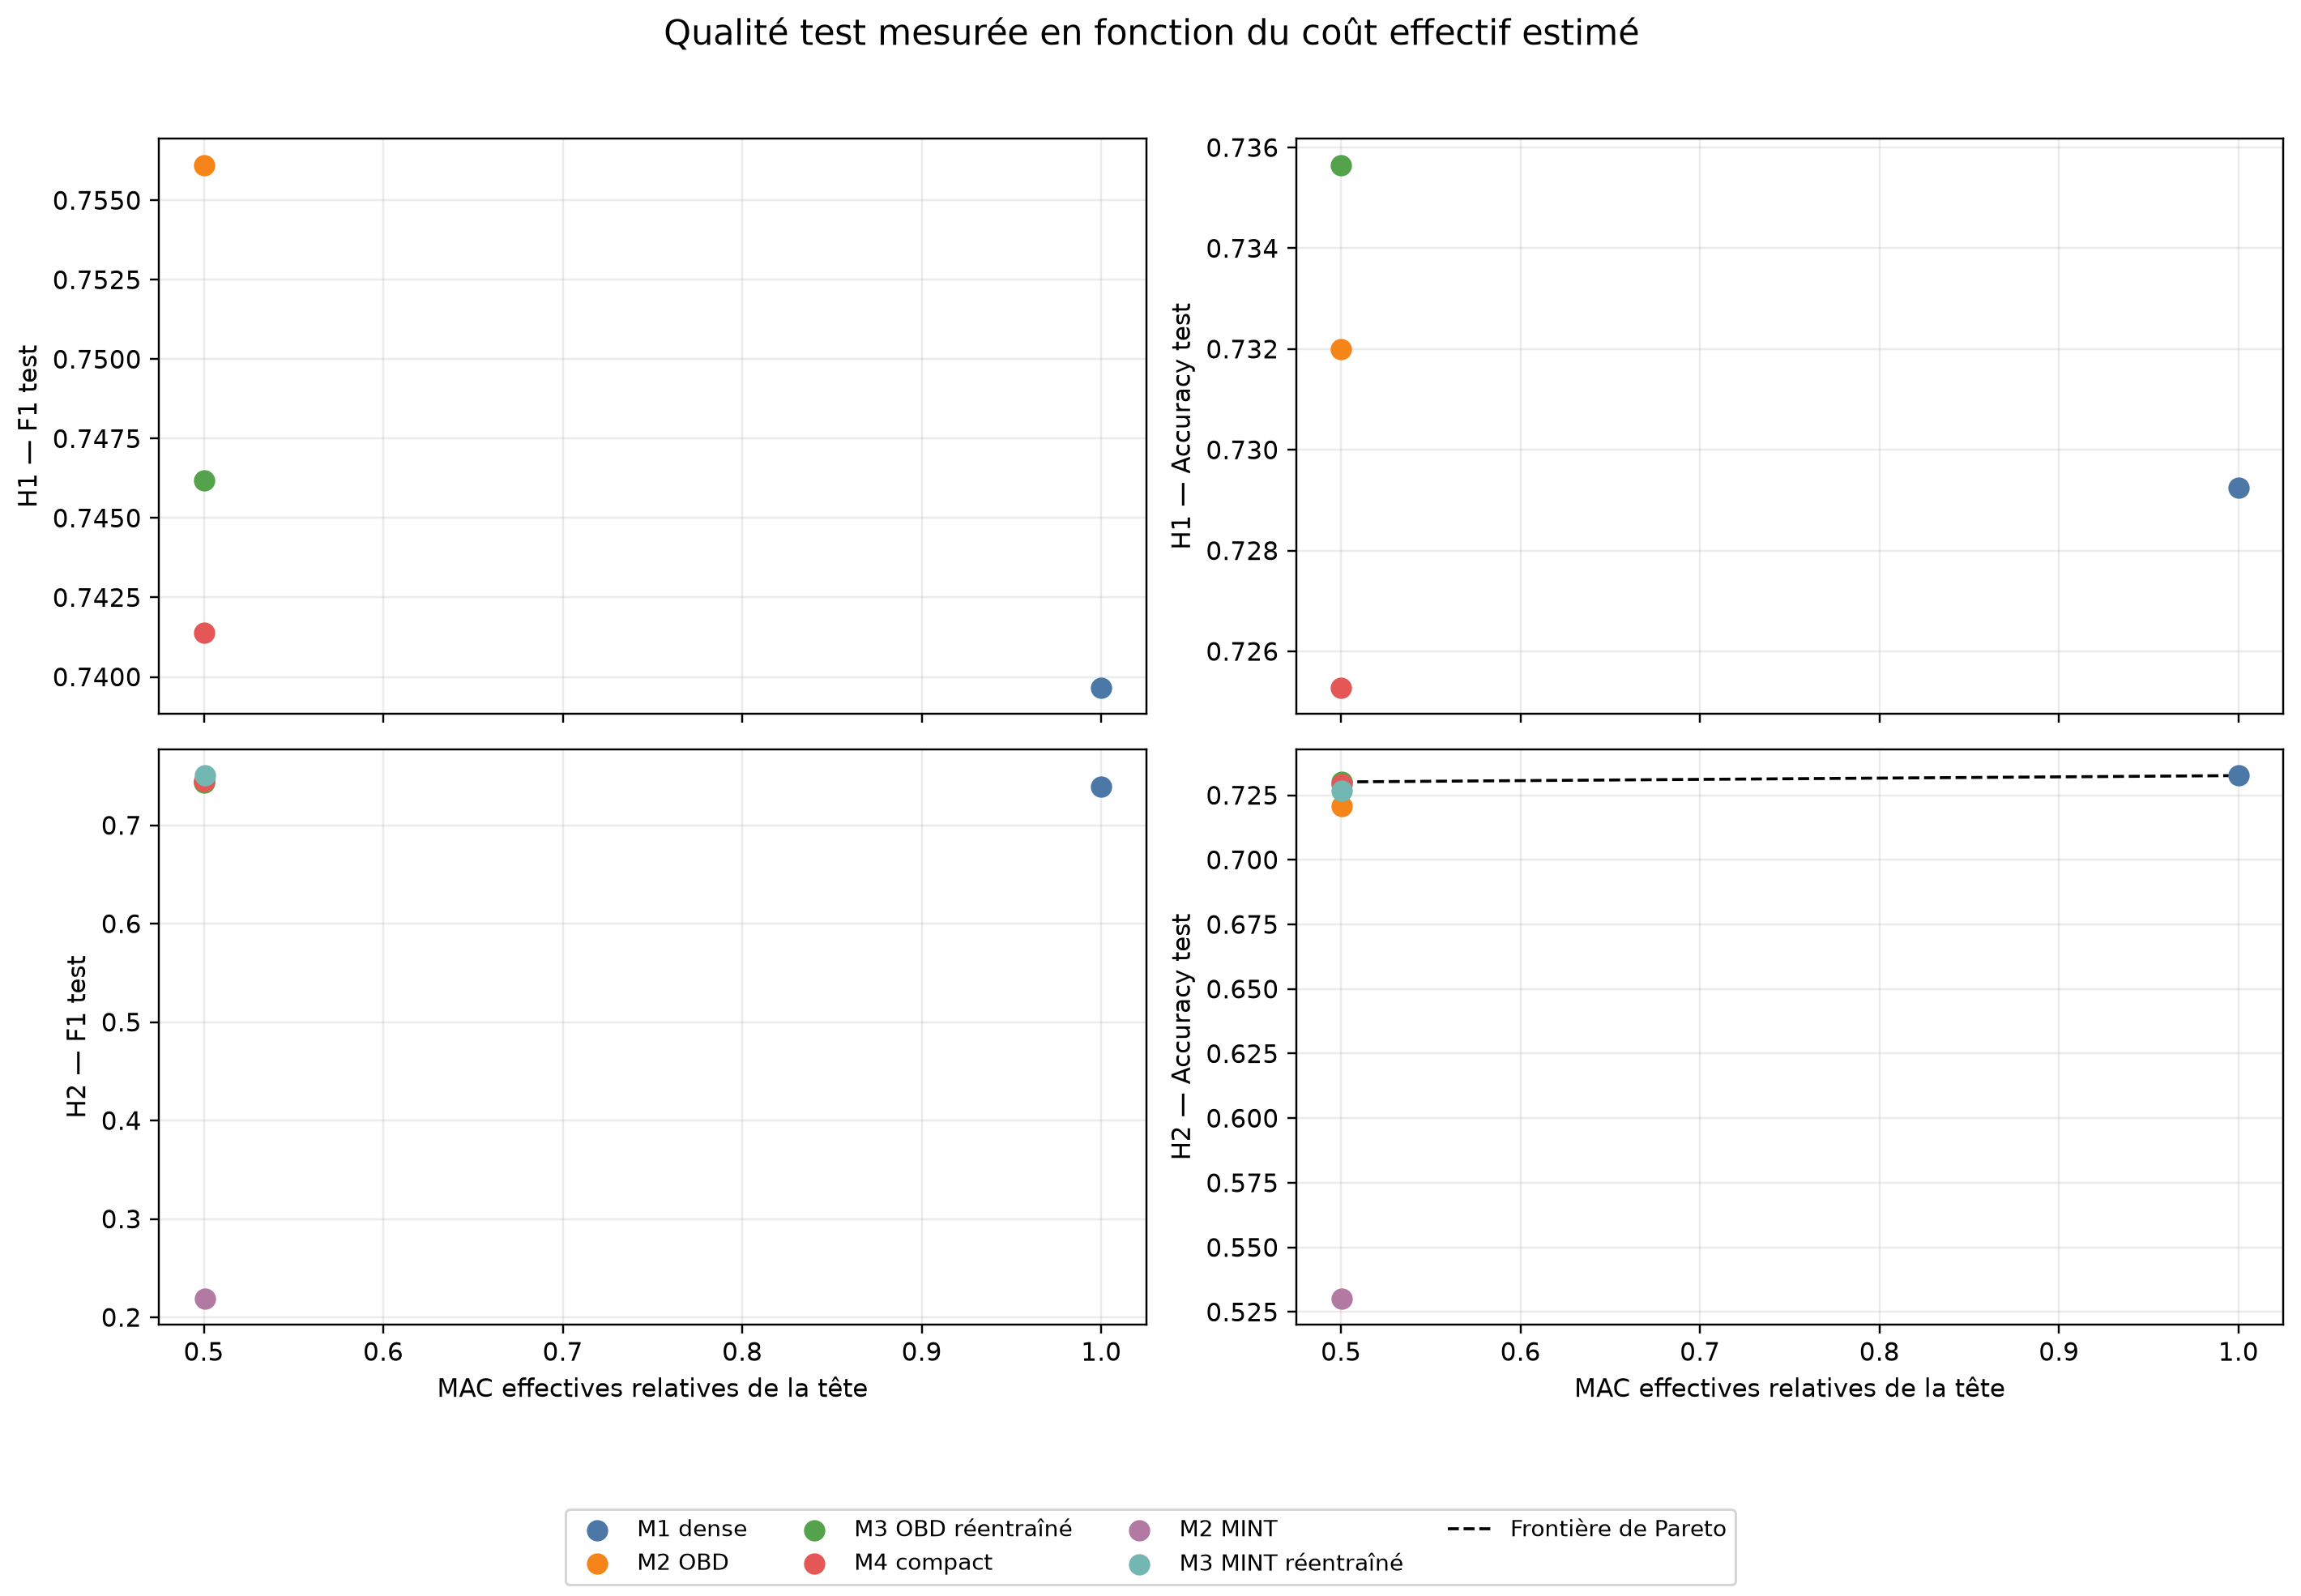
\includegraphics[width=0.96\textwidth]{../figures/experimentales/qualite_calcul_tete_pareto.png}
    \caption{Qualité de test en fonction des MAC effectives idéales de la
    tête. Pour les masques OBD et MINT, l'abscisse suppose qu'un moteur sparse
    sait omettre les multiplications par zéro ; elle ne représente donc pas la
    quantité de calcul réellement exécutée par PyTorch dense.}
    \label{fig:resultats_pareto_calcul}
\end{figure}

Dans la vue tête seule, toutes les solutions réduites se situent près de
$50\,\%$ du coût de M1. La qualité permet alors de les départager : H1/M2 et
H2/MINT-M3 maximisent le F1, tandis que H1/M3 et H2/M1 maximisent l'accuracy.
Le passage à la vue pipeline rapproche horizontalement les solutions de M1,
mais ne change pas leur ordre. Ces courbes répondent à la question du nombre
de paramètres ou de MAC \emph{potentiellement} évitables ; elles ne suffisent
pas à conclure sur le déploiement.

\subsection{Critères ajustés et sensibilité au coefficient alpha}
\label{ssec:resultats_ajustes}

\begin{figure}[!htbp]
    \centering
    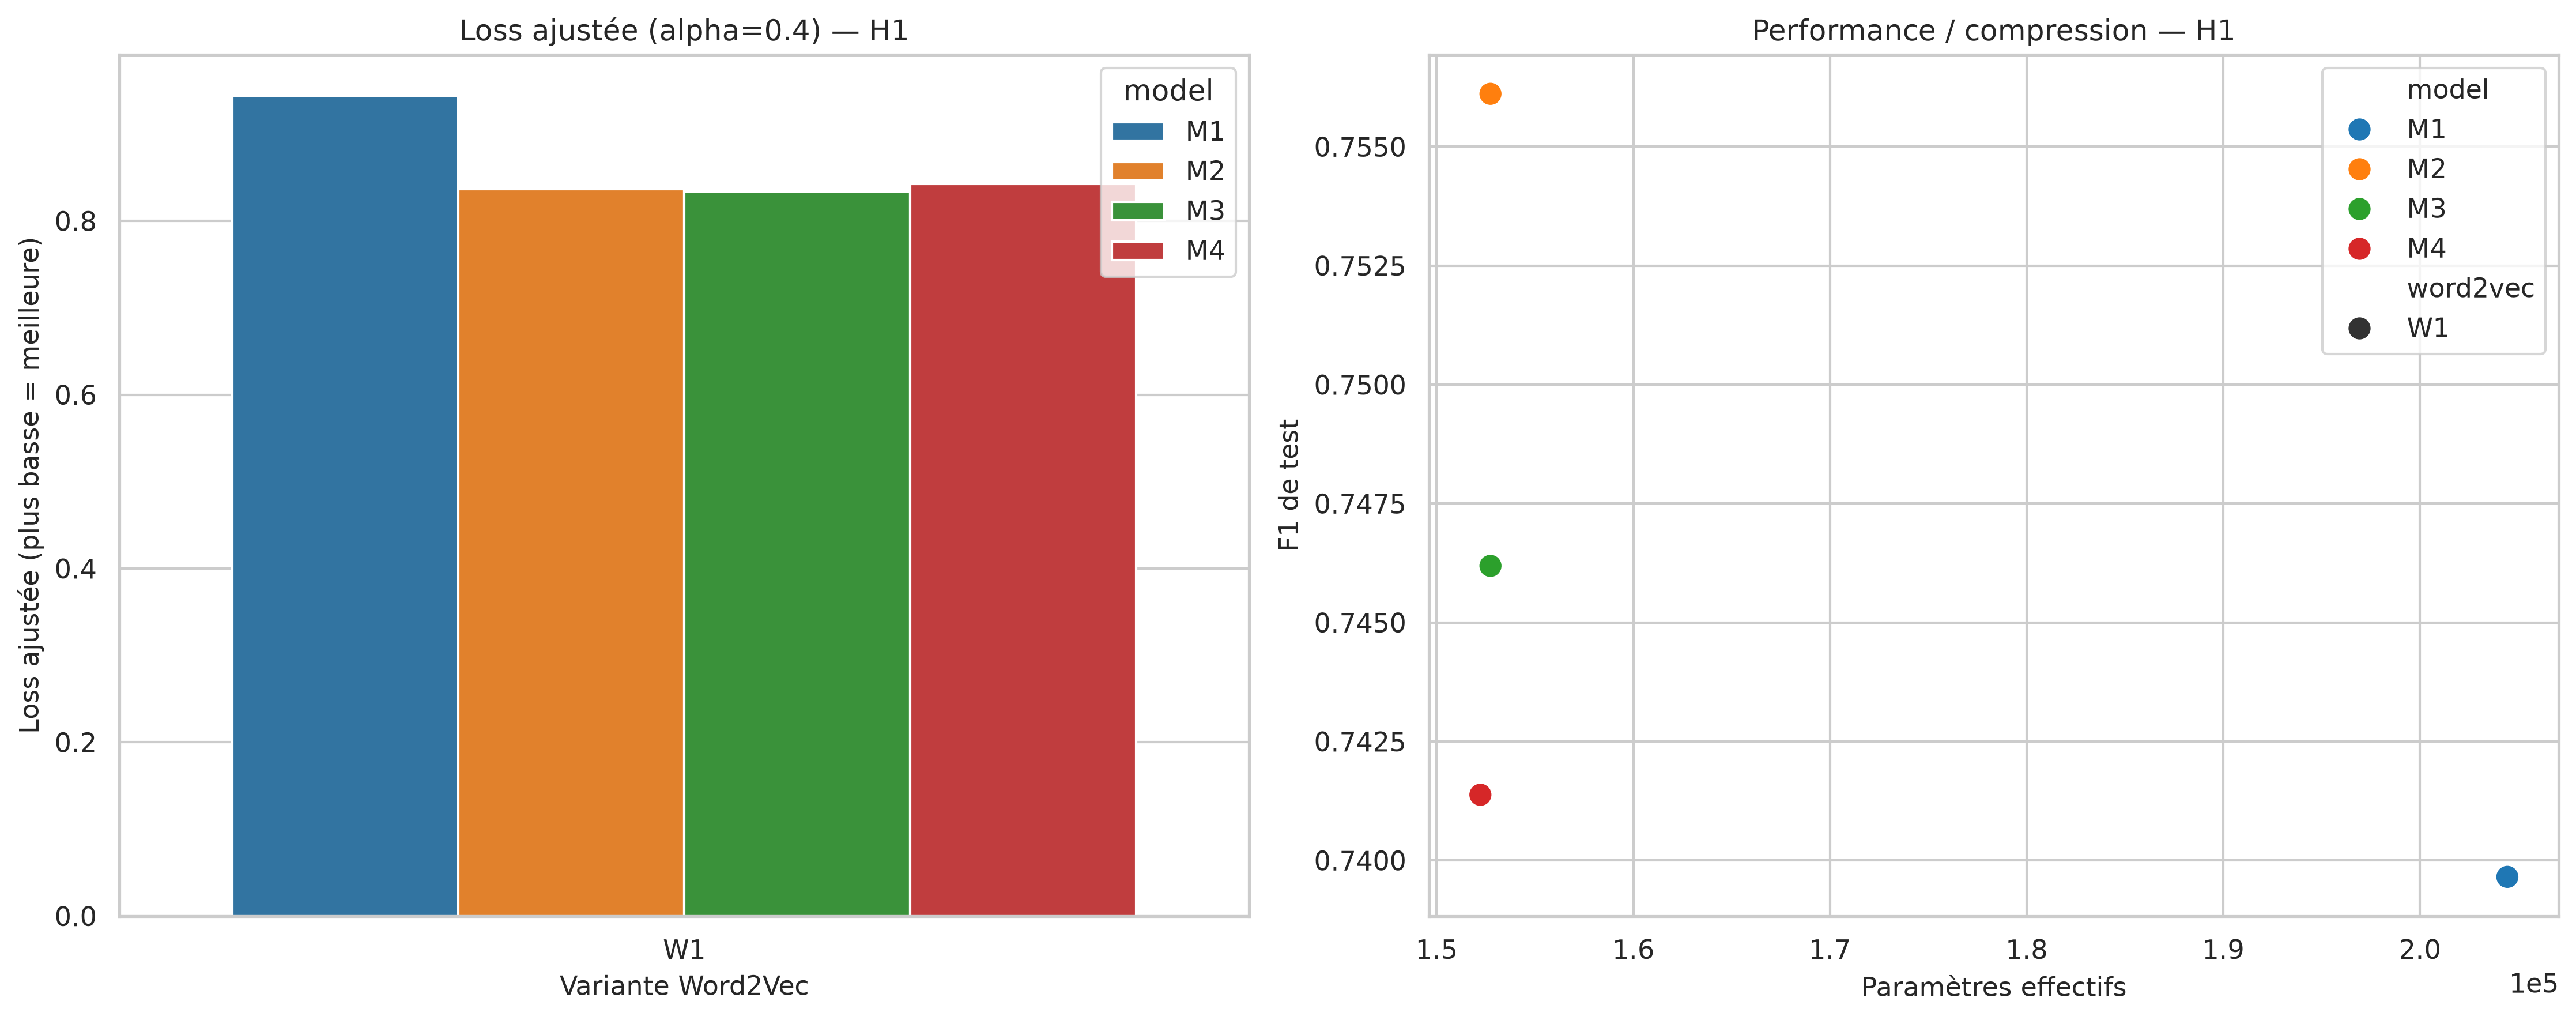
\includegraphics[width=0.94\textwidth]{../figures/experimentales/adjusted_loss_benchmark_H1.png}
    \par\smallskip\small (a) H1.\par\medskip
    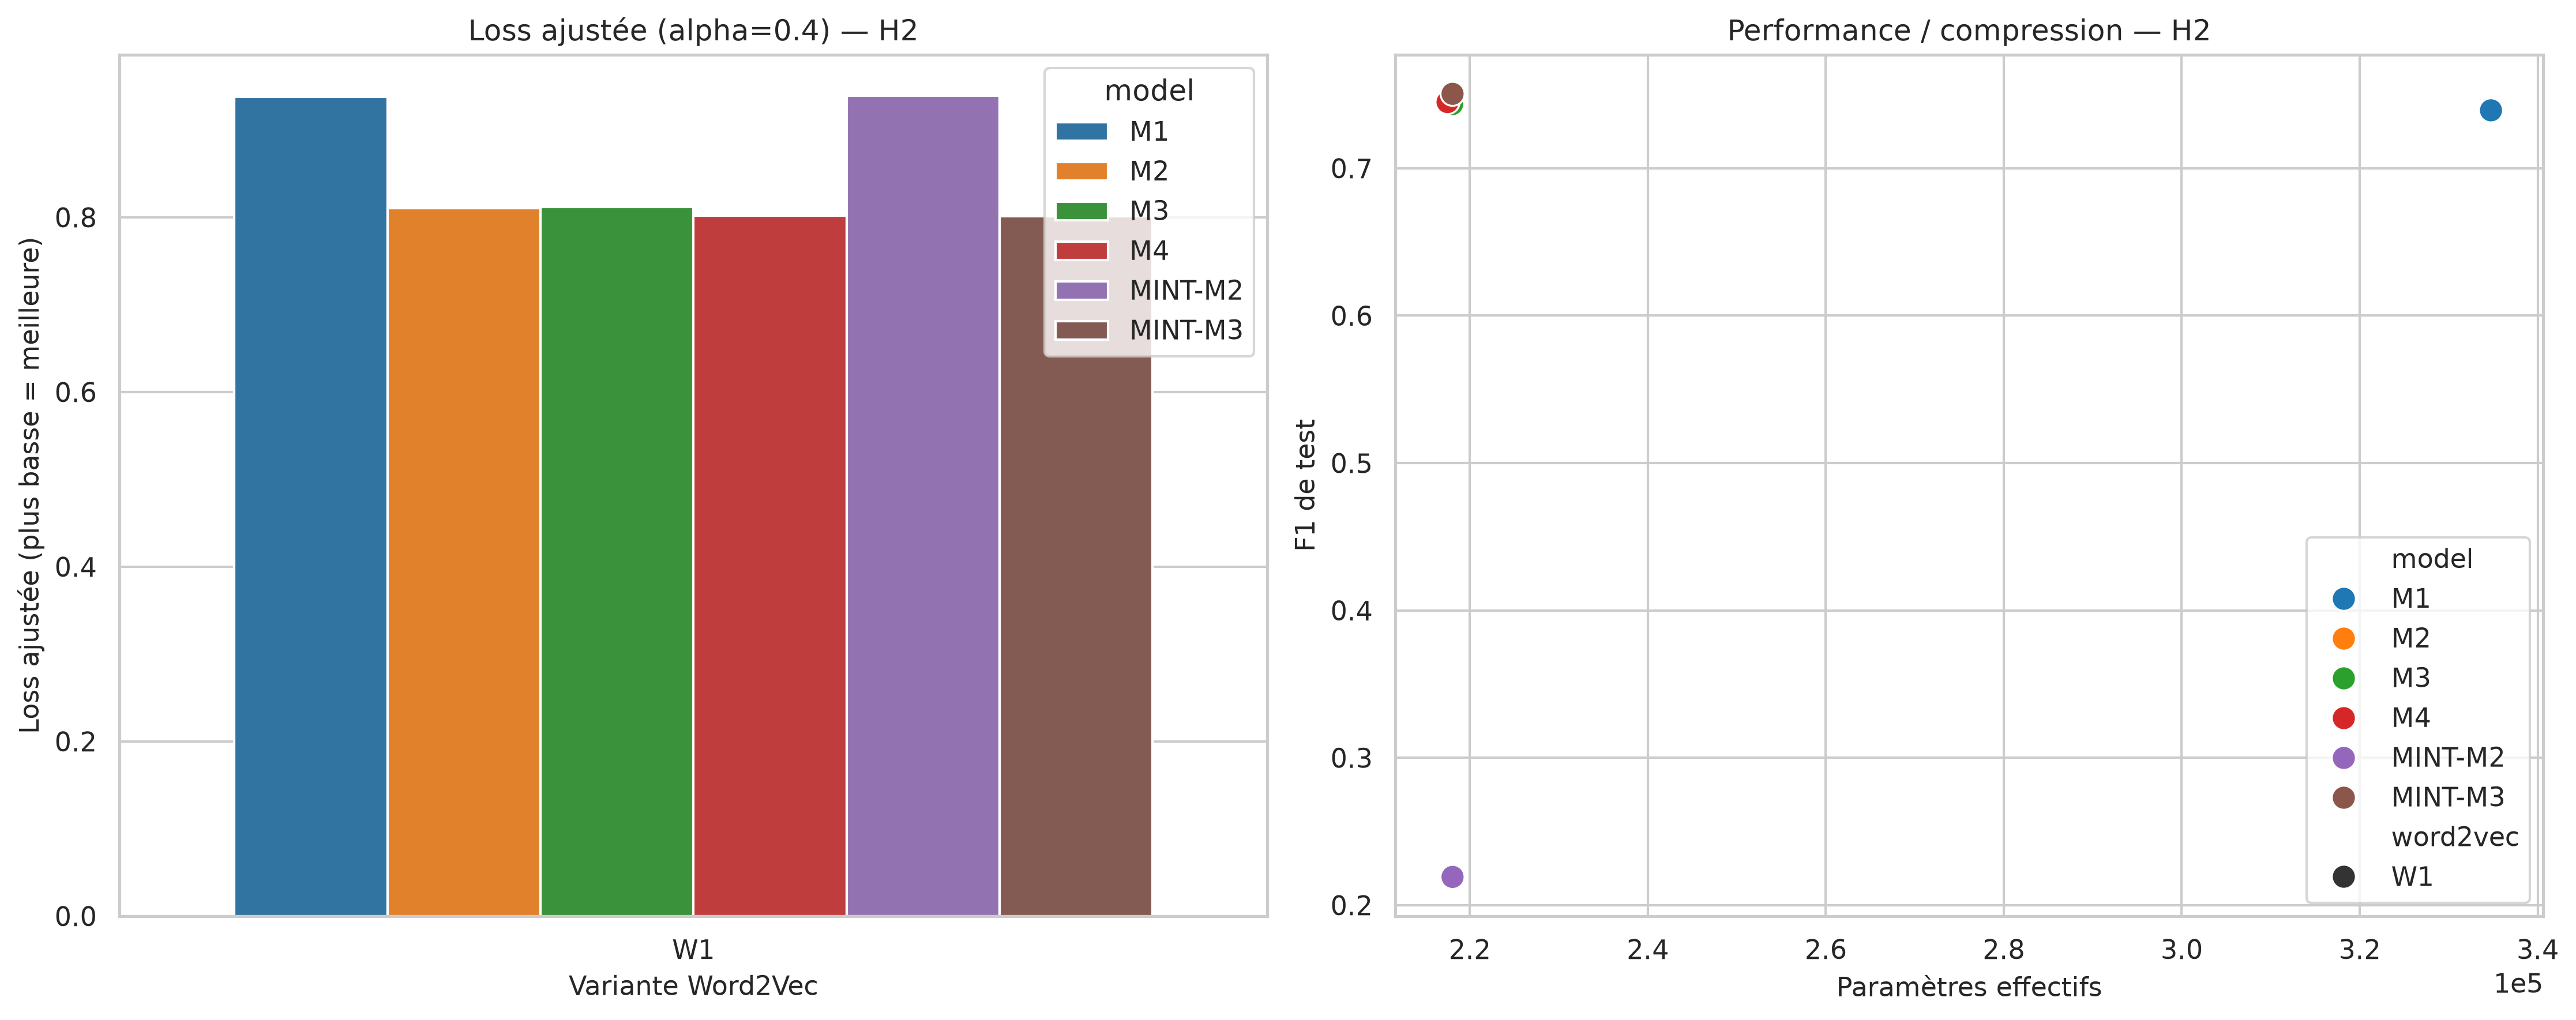
\includegraphics[width=0.94\textwidth]{../figures/experimentales/adjusted_loss_benchmark_H2.png}
    \par\smallskip\small (b) H2.
    \caption{Loss ajustée (à gauche) et F1 brut en fonction des paramètres
    effectifs (à droite). L'ajustement repose sur le nombre de paramètres
    effectifs du pipeline, backbone compris :
    $\mathcal{L}_{\text{ajustée}}=\mathcal{L}_{\mathrm{test}}+
    0{,}4\,P_{\mathrm{pipeline}}^{\mathrm{eff}}/
    P_{\mathrm{pipeline}}^{\mathrm{M1}}$. Il ne dépend pas du nombre de MAC ;
    une loss ajustée plus faible est meilleure.}
    \label{fig:resultats_loss_ajustee}
\end{figure}

Avec $\alpha=0{,}4$, H1/M3 obtient la plus faible loss ajustée
($0{,}8342$), devant M2 ($0{,}8367$) et M4 ($0{,}8428$). Pour H2, MINT-M3
($0{,}8015$) et M4 ($0{,}8018$) sont pratiquement à égalité. M1 conserve la
meilleure loss brute de H2, mais sa pénalisation de complexité porte sa loss
ajustée à $0{,}9381$. MINT-M2 reste mauvais ($0{,}9392$) : réduire le nombre
de poids ne compense pas une perte prédictive aussi importante.

\begin{figure}[!htbp]
    \centering
    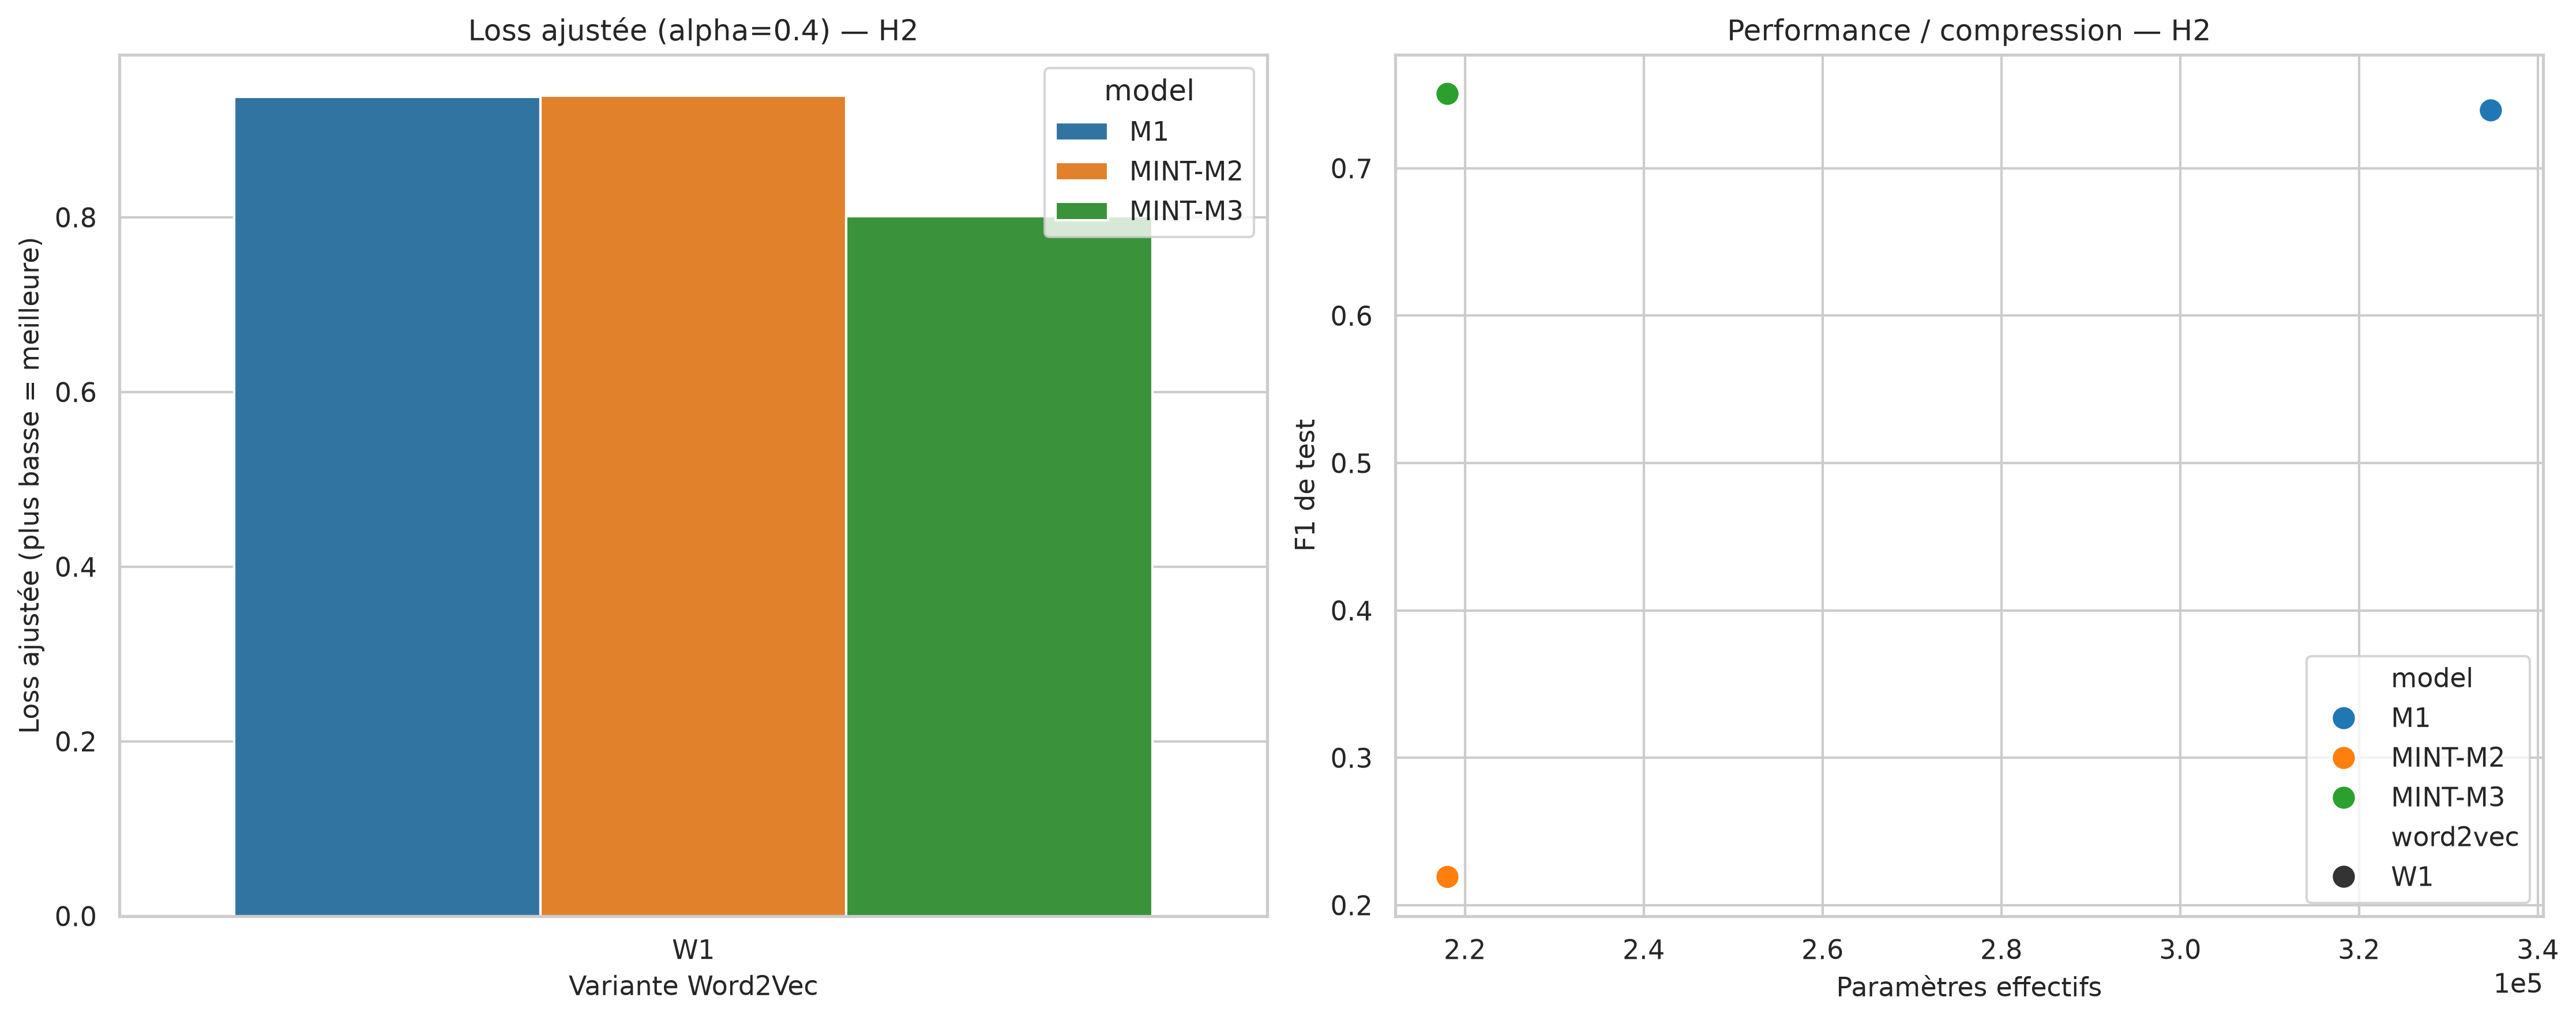
\includegraphics[width=0.9\textwidth]{../figures/experimentales/adjusted_loss_mint_W1_H2.png}
    \caption{Vue ciblée de la loss ajustée pour M1, MINT-M2 et MINT-M3.
    L'ajustement pénalise le nombre de paramètres effectifs du pipeline,
    backbone compris, et non le nombre de MAC. Cette figure isole l'effet du
    réentraînement à masque MINT constant : M2 et M3 ont le même nombre de
    paramètres, donc toute leur différence provient de la qualité retrouvée
    pendant la cicatrisation.}
    \label{fig:resultats_loss_ajustee_mint}
\end{figure}

\begin{figure}[!htbp]
    \centering
    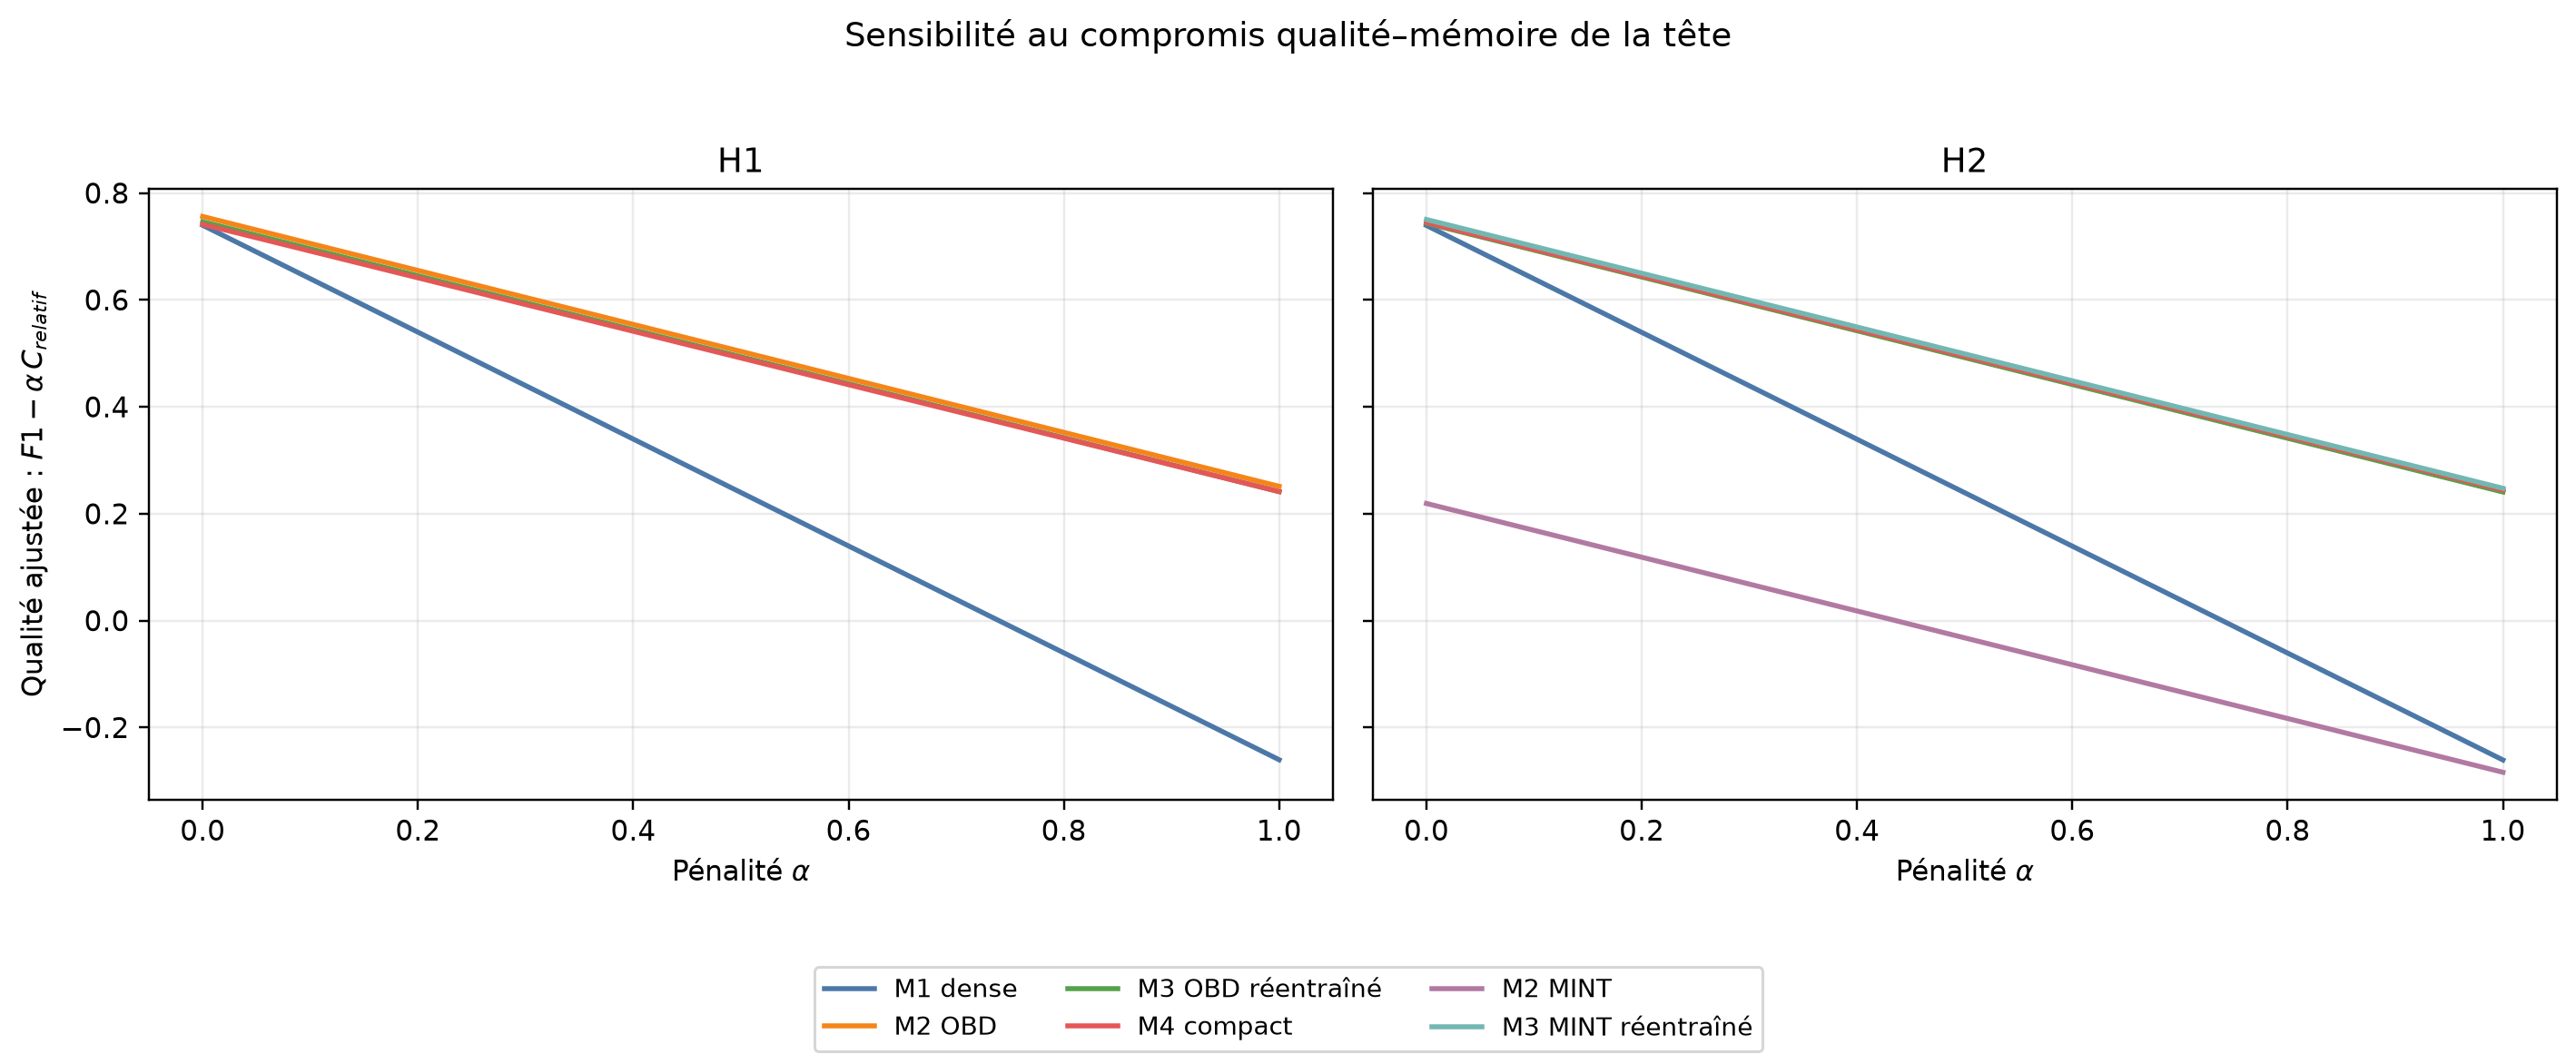
\includegraphics[width=0.94\textwidth]{../figures/experimentales/qualite_ajustee_memoire_tete.png}
    \caption{F1 ajusté en fonction de $\alpha$ à partir du nombre de paramètres
    effectifs de la tête :
    $F1_{\text{ajusté}}=F1-\alpha\,
    P_H^{\mathrm{eff}}/P_H^{\mathrm{M1}}$. L'ajustement porte donc sur les
    paramètres, et non sur les MAC. Sur $[0,1]$, H1/M2 et H2/MINT-M3 restent
    les meilleures solutions.}
    \label{fig:resultats_f1_ajuste_memoire_tete}
\end{figure}

\begin{figure}[!htbp]
    \centering
    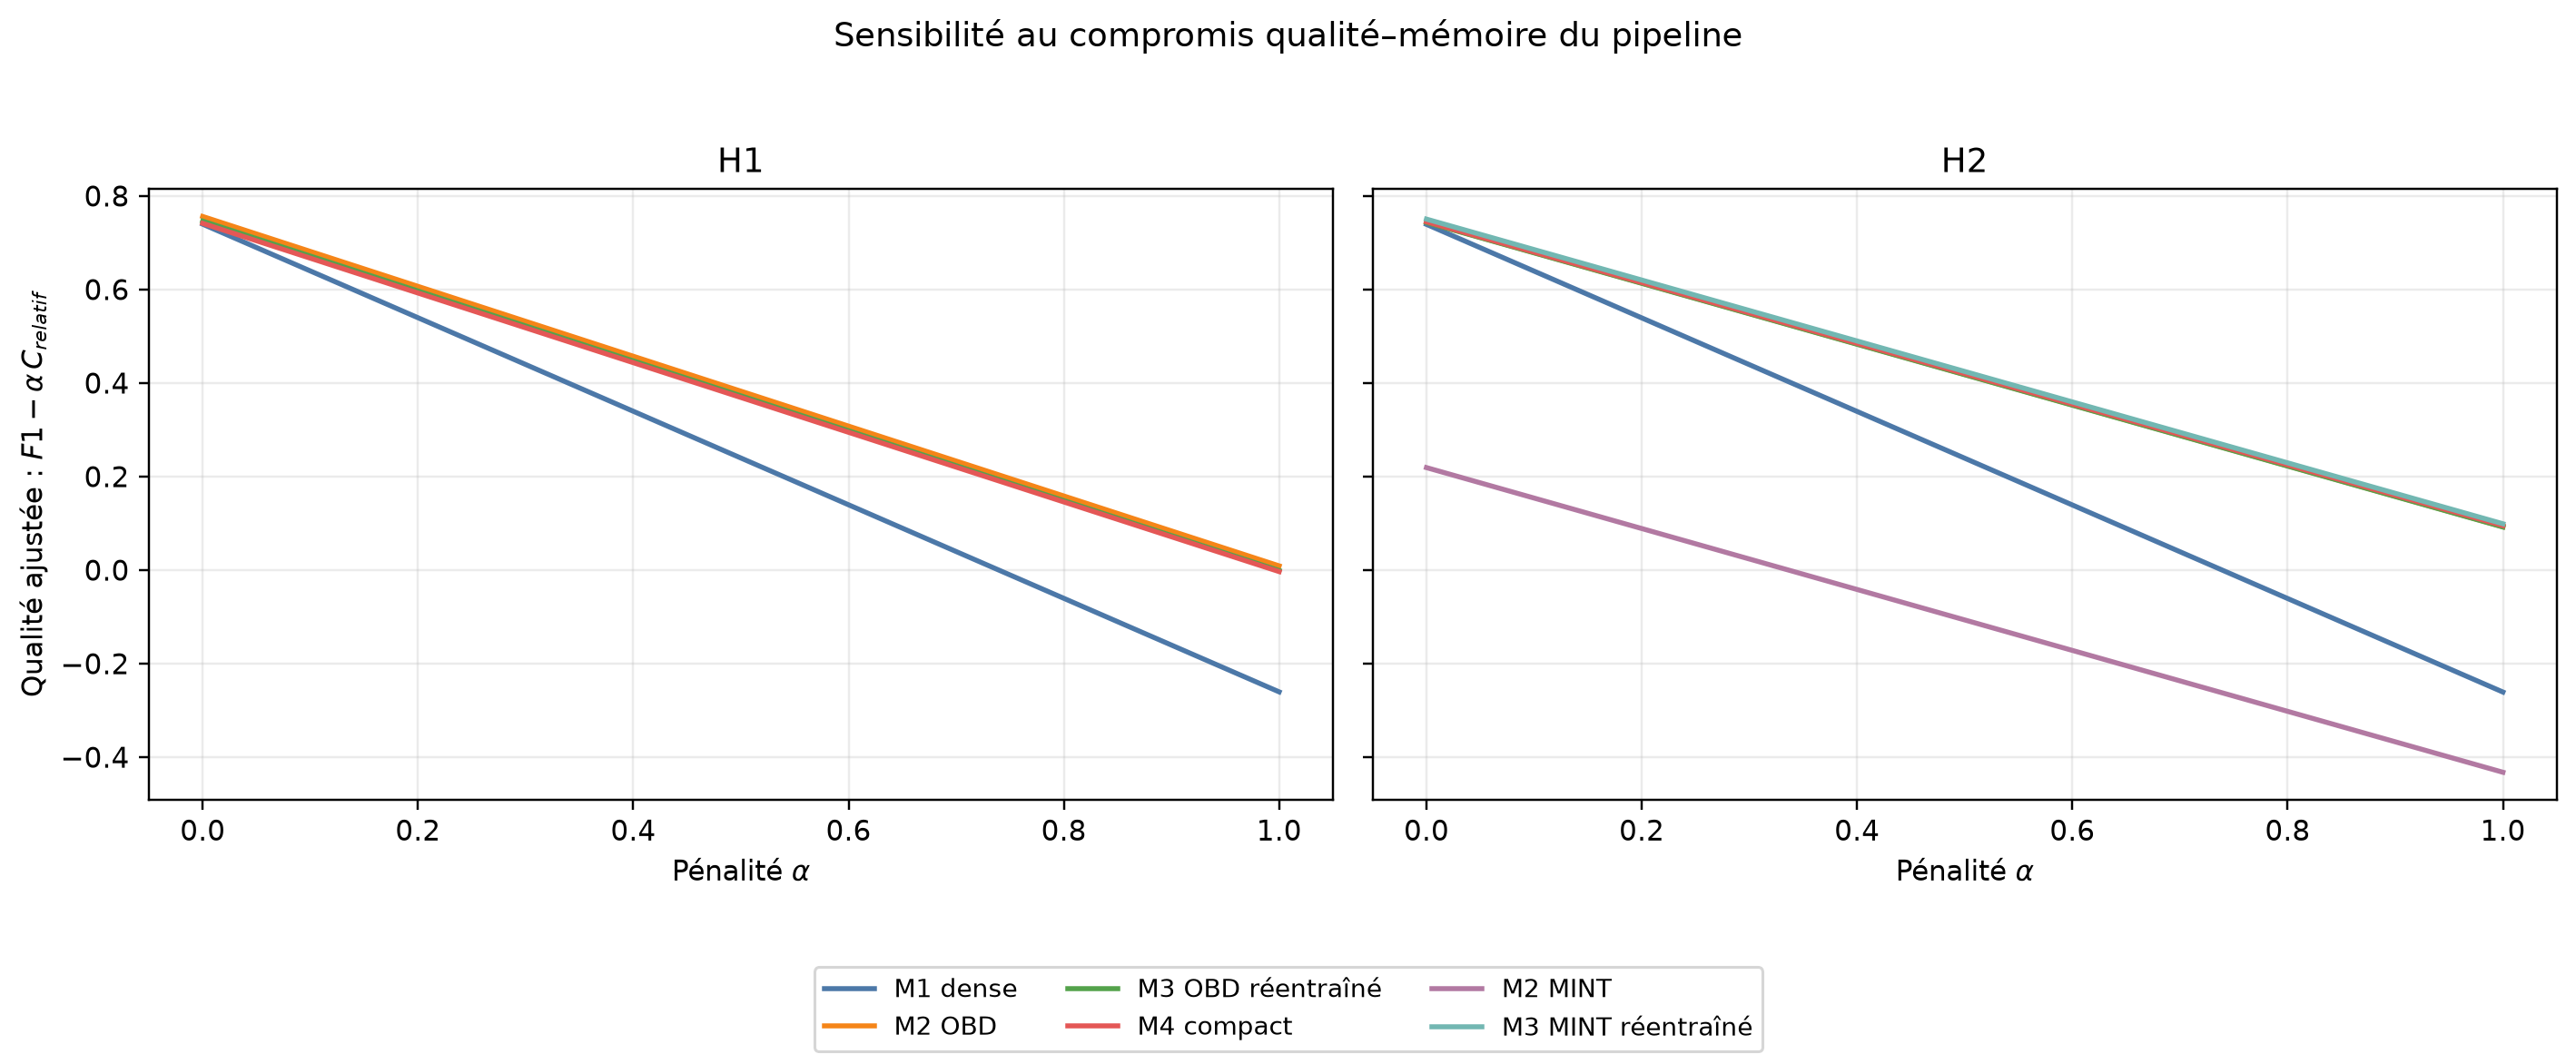
\includegraphics[width=0.94\textwidth]{../figures/experimentales/qualite_ajustee_memoire_pipeline.png}
    \caption{F1 ajusté à partir du nombre de paramètres effectifs du pipeline
    complet : $F1_{\text{ajusté}}=F1-\alpha\,
    P_{\mathrm{pipeline}}^{\mathrm{eff}}/
    P_{\mathrm{pipeline}}^{\mathrm{M1}}$. Cet ajustement porte sur les
    paramètres, et non sur les MAC. Le coût fixe de W1 réduit la pente par
    rapport à la vue tête seule.}
    \label{fig:resultats_f1_ajuste_memoire_pipeline}
\end{figure}

La \autoref{fig:resultats_f1_ajuste_memoire_tete} et la
\autoref{fig:resultats_f1_ajuste_memoire_pipeline} ajustent le F1 à partir du
nombre de paramètres. La \autoref{fig:resultats_f1_ajuste_calcul} utilise au
contraire le coût de calcul : la pénalité est le ratio entre le nombre de MAC
effectives idéales de la tête considérée et celui de la tête dense M1. Cette
quantité représente des opérations théoriquement évitables ; elle ne correspond
pas à la latence mesurée, puisque les couches PyTorch restent denses.

\begin{figure}[!htbp]
    \centering
    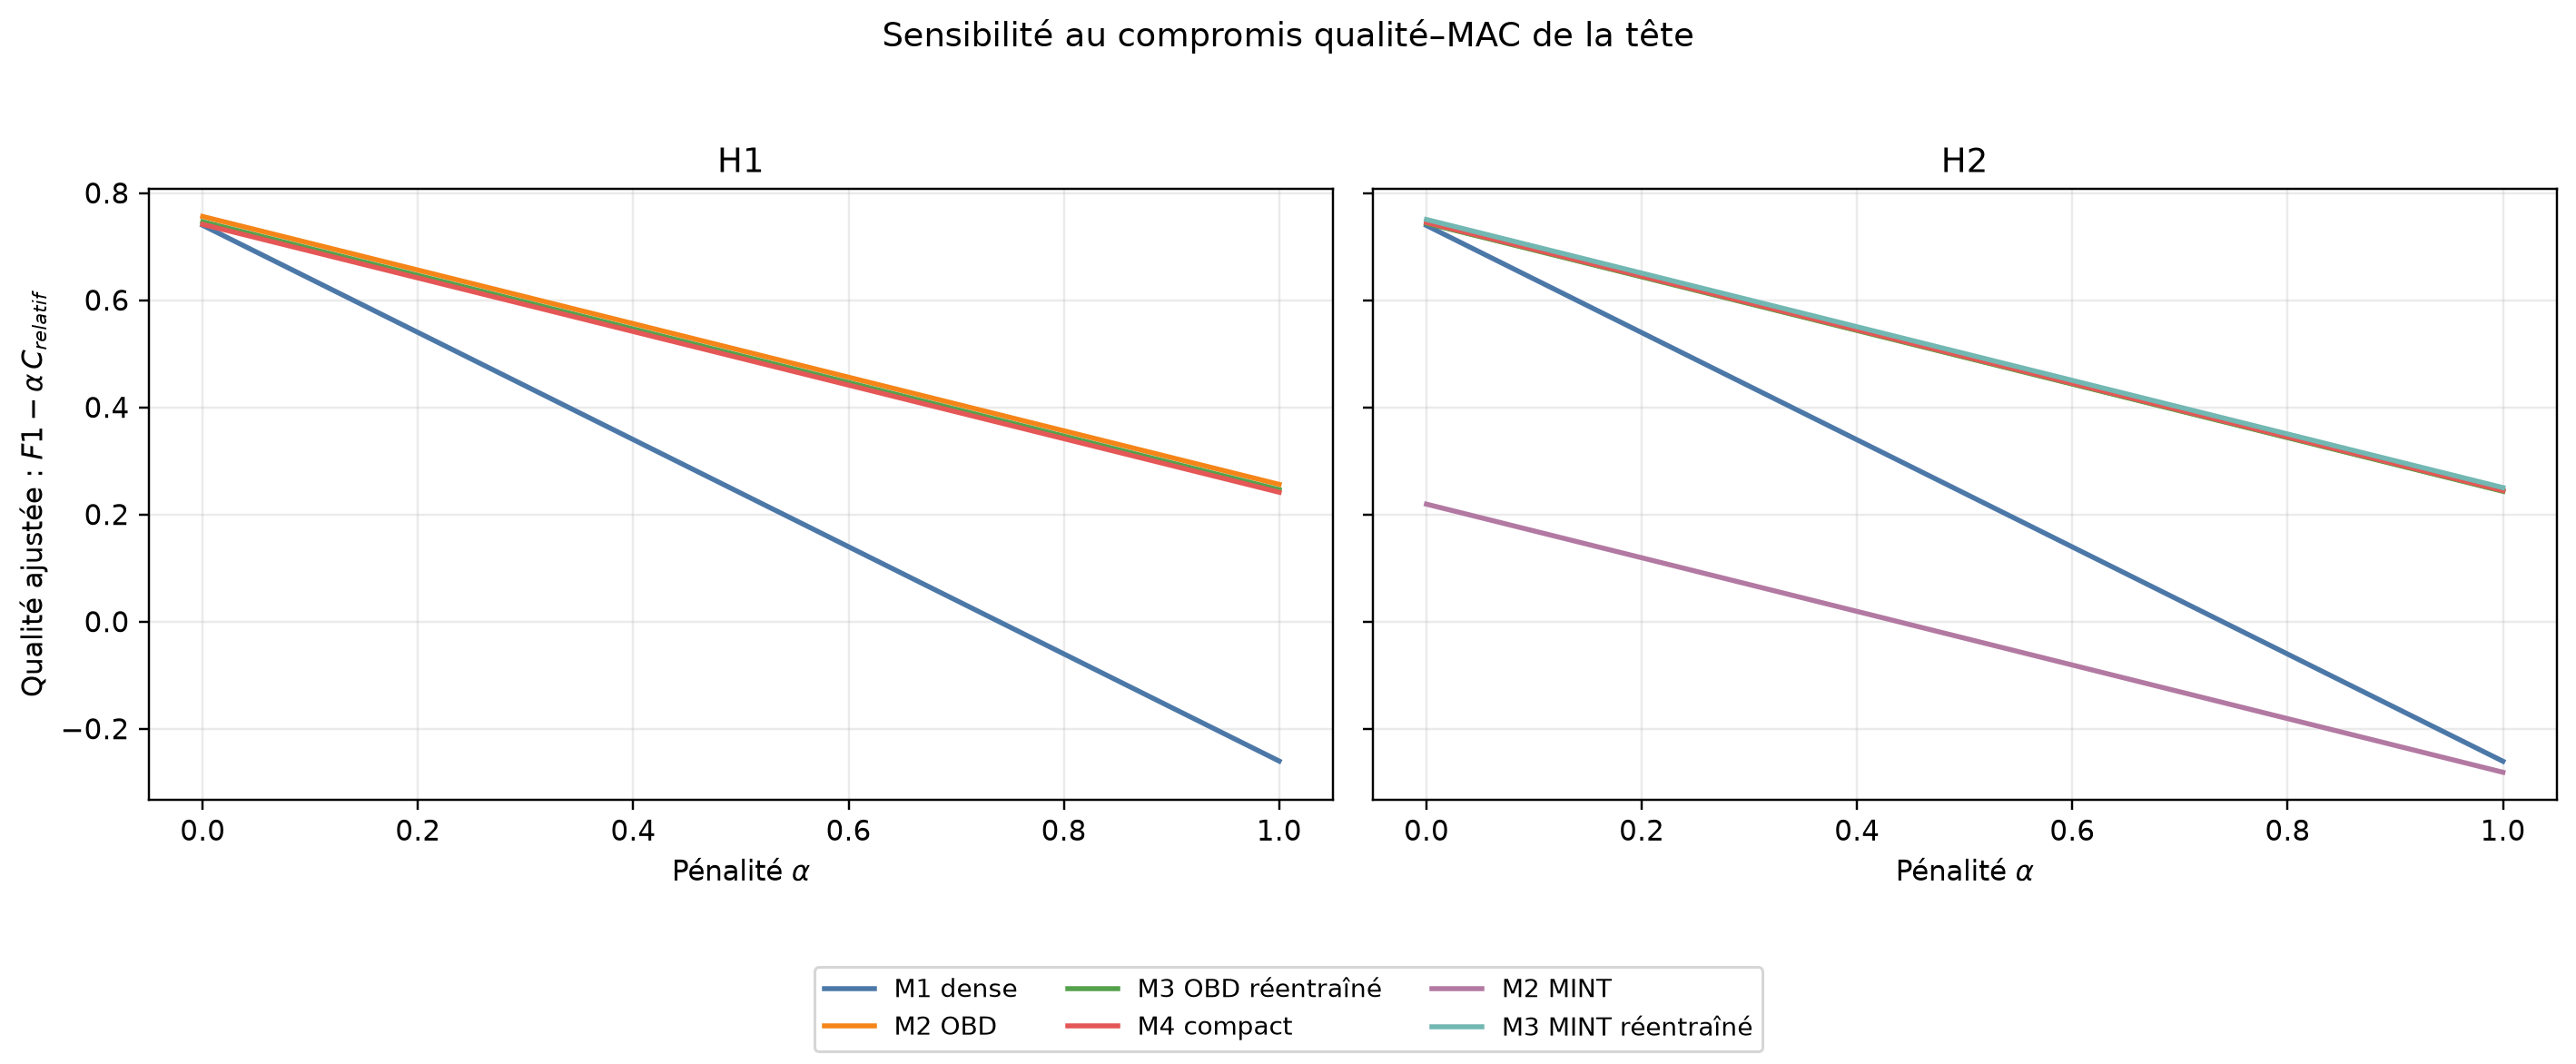
\includegraphics[width=0.94\textwidth]{../figures/experimentales/qualite_ajustee_calcul_tete.png}
    \caption{F1 ajusté à partir du nombre d'opérations de la tête, exprimé en
    MAC effectives idéales : $F1_{\text{ajusté}}=F1-\alpha\,
    C_H^{\mathrm{eff}}/C_H^{\mathrm{M1}}$. Cet ajustement porte donc sur les
    opérations, et non sur le nombre de paramètres. Les courbes restent proches
    de celles de la mémoire tête seule, car chaque poids actif d'une couche
    linéaire correspond ici à une MAC potentielle.}
    \label{fig:resultats_f1_ajuste_calcul}
\end{figure}

\paragraph{Synthèse selon l'accuracy ajustée.}
Pour compléter les courbes de F1, le tableau~\ref{tab:accuracy_ajustee} applique le
même principe à l'accuracy de test avec $\alpha=0{,}4$. Les trois scores sont
respectivement pénalisés par le ratio de paramètres effectifs de la tête, le
ratio de paramètres effectifs du pipeline et le ratio de MAC effectives idéales
de la tête, chaque ratio étant normalisé par M1. Ces valeurs sont des critères
de classement, et non des pourcentages d'accuracy.

\begin{table}[!htbp]
    \centering
    \resizebox{\textwidth}{!}{%
    \begin{tabular}{|l|l|r|r|r|r|}
        \hline
        Tête & Modèle & Accuracy brute &
        $\mathrm{Acc}_{\alpha}^{P_H}$ &
        $\mathrm{Acc}_{\alpha}^{P_{\mathrm{pipeline}}}$ &
        $\mathrm{Acc}_{\alpha}^{\mathrm{MAC}_H}$ \\ \hline
        H1 & M1     & $72{,}92\,\%$ & $0{,}3292$ & $0{,}3292$ & $0{,}3292$ \\ \hline
        H1 & M2 OBD & $73{,}20\,\%$ & $0{,}5300$ & $0{,}4332$ & $0{,}5320$ \\ \hline
        H1 & M3 OBD & $73{,}57\,\%$ & $\mathbf{0{,}5337}$ & $\mathbf{0{,}4368}$ & $\mathbf{0{,}5357}$ \\ \hline
        H1 & M4     & $72{,}53\,\%$ & $0{,}5253$ & $0{,}4275$ & $0{,}5253$ \\ \hline
        H2 & M1     & $73{,}26\,\%$ & $0{,}3326$ & $0{,}3326$ & $0{,}3326$ \\ \hline
        H2 & M2 OBD & $72{,}07\,\%$ & $0{,}5196$ & $0{,}4602$ & $0{,}5206$ \\ \hline
        H2 & M3 OBD & $73{,}02\,\%$ & $\mathbf{0{,}5291}$ & $\mathbf{0{,}4696}$ & $\mathbf{0{,}5300}$ \\ \hline
        H2 & M4     & $72{,}92\,\%$ & $0{,}5290$ & $0{,}4693$ & $0{,}5291$ \\ \hline
        H2 & MINT-M2 & $53{,}02\,\%$ & $0{,}3291$ & $0{,}2697$ & $0{,}3300$ \\ \hline
        H2 & MINT-M3 & $72{,}68\,\%$ & $0{,}5256$ & $0{,}4662$ & $0{,}5266$ \\ \hline
    \end{tabular}}
    \caption{Accuracy ajustée avec $\alpha=0{,}4$. Les colonnes pénalisent,
    de gauche à droite, le nombre de paramètres effectifs de la tête, le nombre
    de paramètres effectifs du pipeline complet et le nombre de MAC effectives
    idéales de la tête. Les valeurs en gras indiquent le meilleur modèle de
    chaque tête pour le critère considéré.}
    \label{tab:accuracy_ajustee}
\end{table}

OBD-M3 maximise les trois formes d'accuracy ajustée pour H1 comme pour H2. Sur
H2, l'écart avec M4 reste toutefois inférieur à $0{,}001$ pour les trois
critères : ce classement très fin ne doit donc pas être interprété comme un
avantage statistiquement établi avec une seule graine.

Pour les courbes de F1, l'analyse de sensibilité ne fait pas apparaître de
changement de vainqueur sur $\alpha\in[0,1]$. Ce constat ne signifie pas que le choix de $\alpha$ est sans
importance : il résulte du fait que les variantes réduites ont presque toutes
la même cible de capacité. L'intérêt principal de ces figures est alors de
montrer à quelle vitesse M1, plus coûteux, est dominé lorsque la compression
reçoit un poids croissant.

\subsection{Coût hors ligne du scoring}
\label{ssec:resultats_cout_scoring}

\begin{figure}[!htbp]
    \centering
    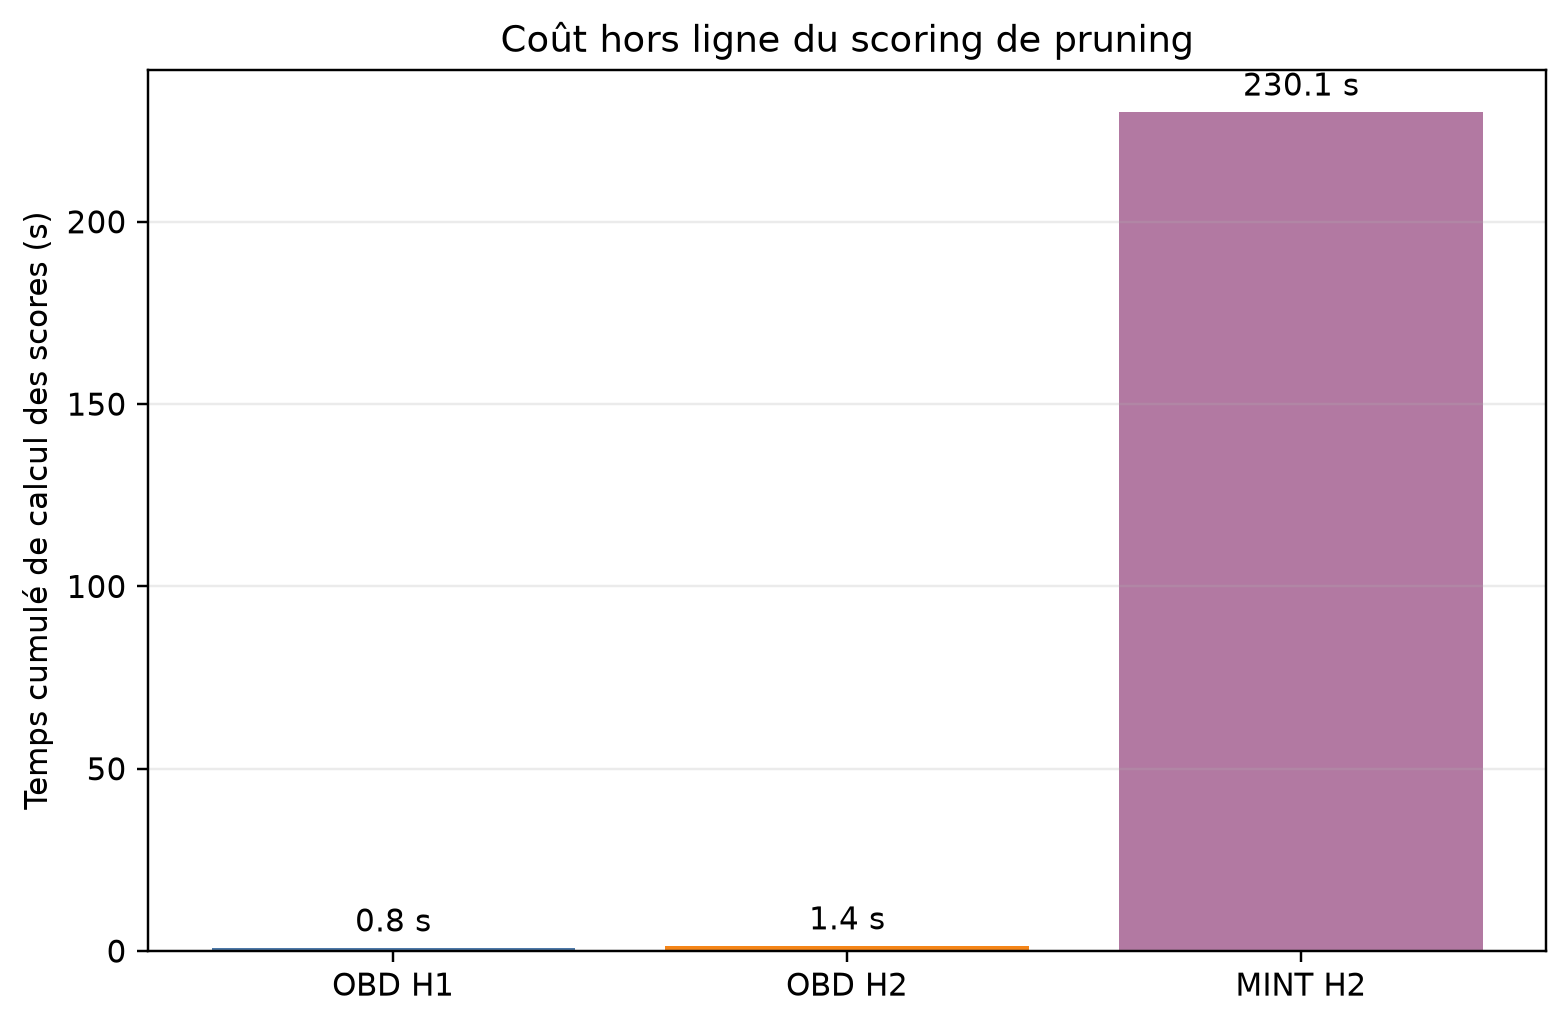
\includegraphics[width=0.78\textwidth]{../figures/experimentales/cout_scoring_pruning.png}
    \caption{Temps cumulé de calcul des scores. OBD inclut tous les tours de
    scoring itératif ; MINT inclut les $12\,296$ estimations GMI de ses trois
    couches, mais pas le réentraînement commun aux comparaisons de qualité.}
    \label{fig:resultats_cout_scoring}
\end{figure}

OBD demande $0{,}85$ seconde pour H1 et $1{,}41$ seconde pour H2. MINT demande
$230{,}1$ secondes sur H2, soit environ 163 fois le temps de scoring OBD de la
même tête. La première couche concentre $186{,}2$ secondes et la deuxième
$43{,}7$ secondes ; la sortie ne demande que $0{,}15$ seconde. Ce déséquilibre
s'explique par le nombre d'unités aval et donc de blocs à scorer. Dans cette
implémentation, le meilleur F1 de MINT-M3 s'accompagne ainsi d'un coût hors
ligne très supérieur.

\subsection{Gains idéaux et gains réellement observés}
\label{ssec:resultats_gains_reels}

Les mesures de latence sont effectuées sur CPU AMD Ryzen AI 9 365, sans CUDA,
avec PyTorch configuré sur 10 threads. Elles utilisent $2\,048$ textes de test
déjà tokenisés, des batches de 512, deux passages d'échauffement et la médiane
de sept répétitions. Le temps par texte est donc un temps \emph{amorti dans un
batch}, et non la latence d'une requête isolée. Le temps du pipeline additionne
l'agrégation des embeddings et la tête ; la tokenisation est exclue. La taille
mesurée est celle d'un artefact d'inférence dense contenant la table d'entrée
W1 et l'état du classifieur, sans table CBOW de sortie ni masque auxiliaire.

\begin{table}[!htbp]
    \centering
    \begin{tabular}{|l|l|r|r|r|}
        \hline
        Tête & Modèle & Tête ($\mu$s/texte) & Pipeline ($\mu$s/texte) & Artefact (KiB) \\ \hline
        H1 & M1 & $3{,}350$ & $16{,}432$ & $801{,}0$ \\ \hline
        H1 & M2 OBD & $3{,}195$ & $16{,}277$ & $801{,}0$ \\ \hline
        H1 & M3 OBD & $3{,}197$ & $16{,}280$ & $801{,}0$ \\ \hline
        H1 & M4 & $1{,}813$ & $14{,}896$ & $597{,}0$ \\ \hline
        H2 & M1 & $5{,}701$ & $18{,}784$ & $1\,310{,}4$ \\ \hline
        H2 & M2 OBD & $5{,}710$ & $18{,}792$ & $1\,310{,}4$ \\ \hline
        H2 & M3 OBD & $5{,}707$ & $18{,}790$ & $1\,310{,}4$ \\ \hline
        H2 & M4 & $3{,}291$ & $16{,}374$ & $852{,}4$ \\ \hline
        H2 & MINT-M2 & $5{,}704$ & $18{,}786$ & $1\,310{,}4$ \\ \hline
        H2 & MINT-M3 & $5{,}707$ & $18{,}790$ & $1\,310{,}4$ \\ \hline
    \end{tabular}
    \caption{Mesures physiques du format dense actuel. Les faibles différences
    entre variantes de même architecture sont du même ordre que la variabilité
    d'un microbenchmark et ne doivent pas être interprétées comme une
    accélération due aux zéros.}
    \label{tab:resultats_runtime}
\end{table}

\begin{figure}[!htbp]
    \centering
    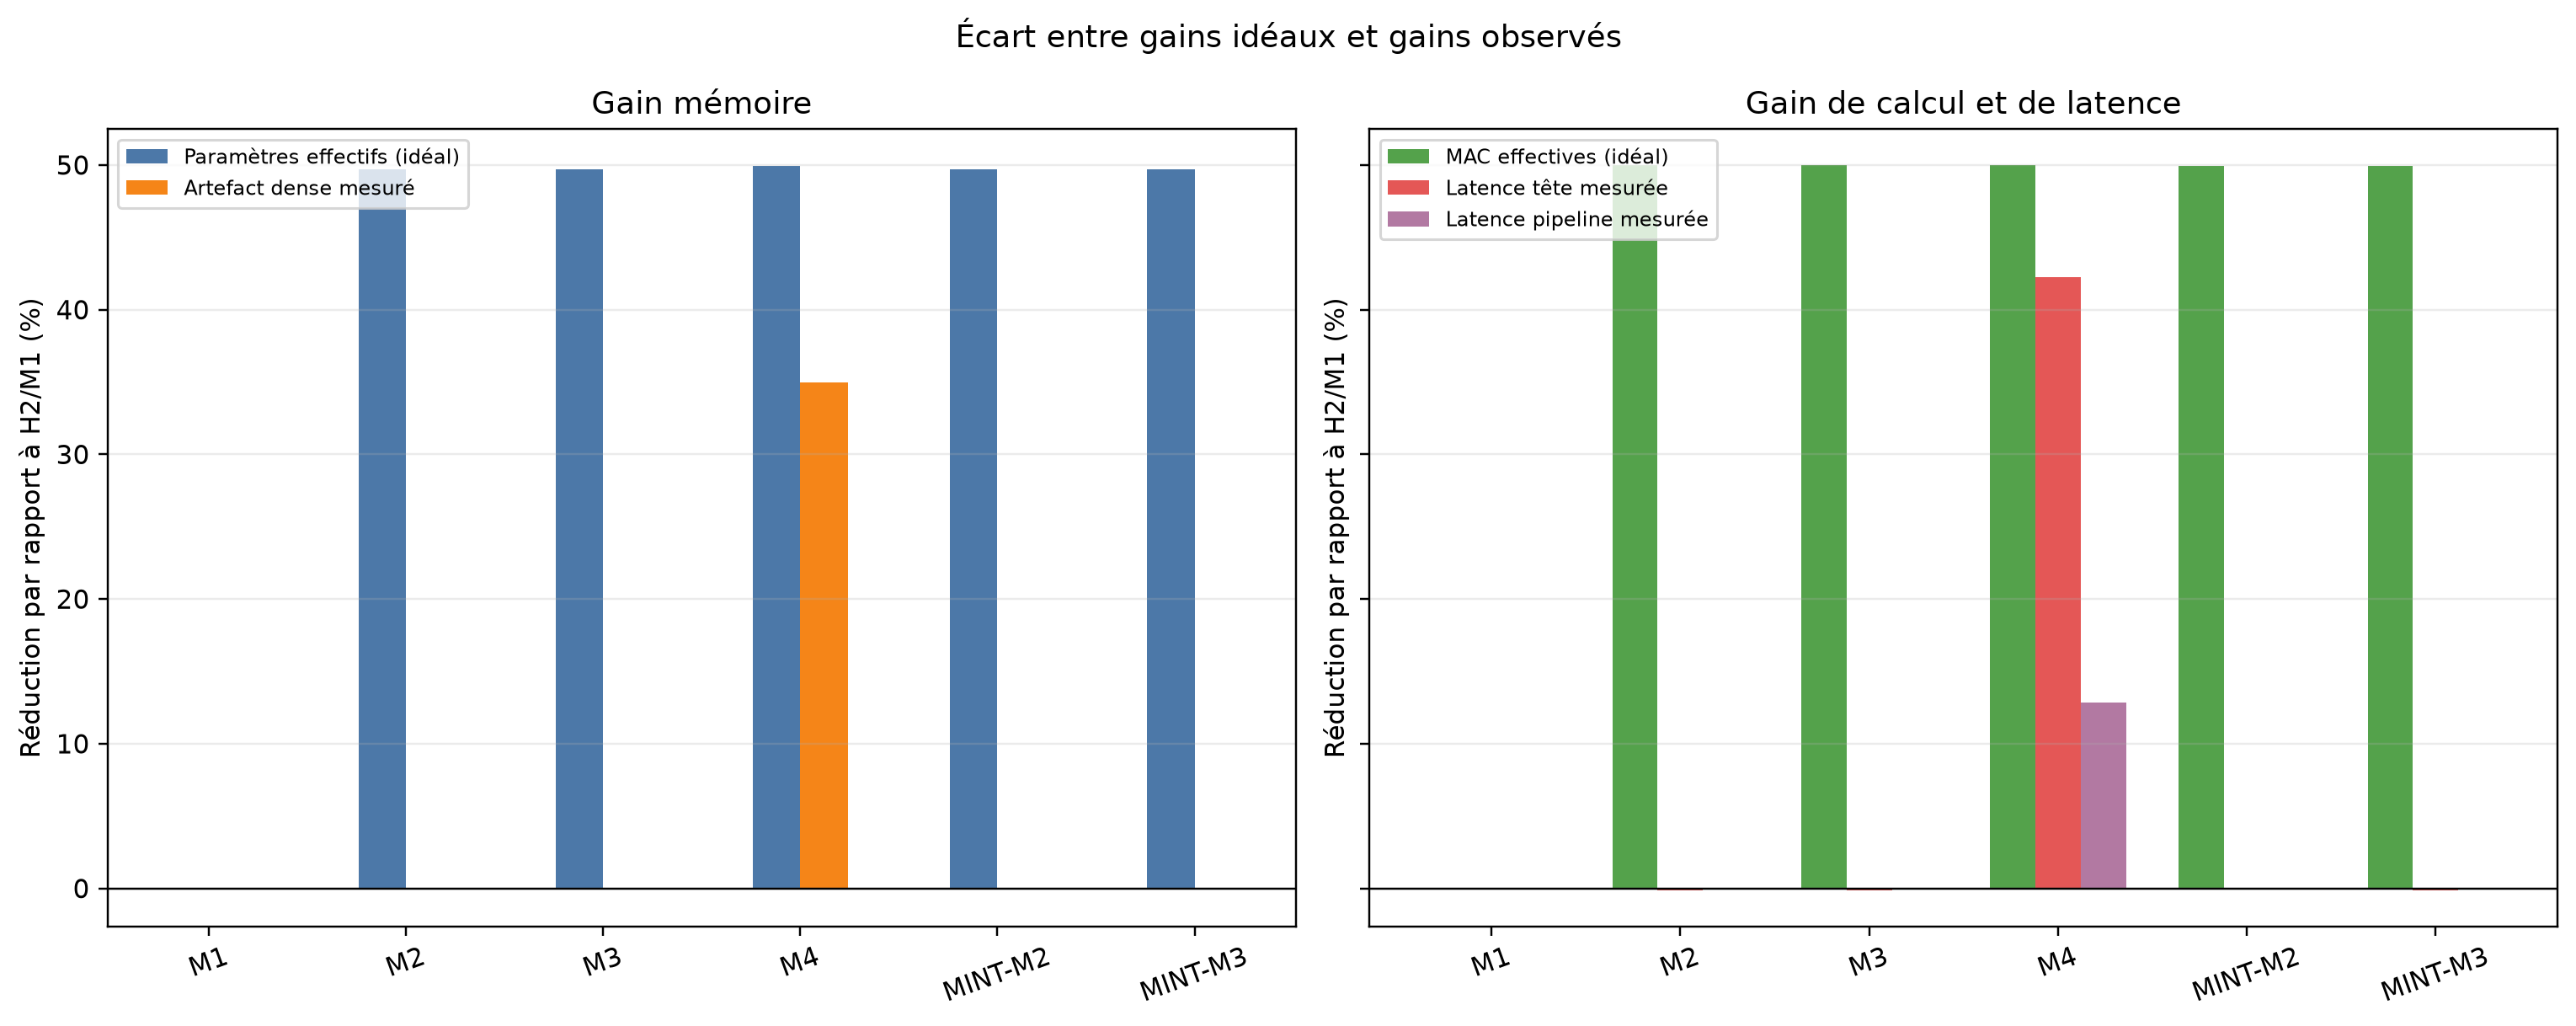
\includegraphics[width=0.96\textwidth]{../figures/experimentales/gain_theorique_vs_reel.png}
    \caption{Réductions idéales et observées pour H2, relativement à M1.
    Les masques OBD et MINT divisent par deux les paramètres et MAC effectifs
    théoriques, mais les tenseurs denses conservent leur taille et leur temps
    d'exécution. Seule M4 modifie physiquement les dimensions.}
    \label{fig:resultats_gain_theorique_reel}
\end{figure}

Le résultat central de la \autoref{fig:resultats_gain_theorique_reel} est
l'absence de gain réel pour les masques. OBD-M2, OBD-M3, MINT-M2 et MINT-M3
occupent exactement la même taille sérialisée que H2/M1 et leurs temps diffèrent
de moins de $0{,}2\,\%$. PyTorch exécute toujours les matrices complètes. M4
réduit au contraire la taille de l'artefact H2 de $34{,}95\,\%$, la latence de
la tête de $42{,}27\,\%$ et celle du pipeline de $12{,}83\,\%$. Pour H1, M4
réduit respectivement ces quantités de $25{,}47\,\%$, $45{,}87\,\%$ et
$9{,}35\,\%$.

Le backbone explique l'écart entre la tête et le pipeline : son agrégation
demande environ $13{,}08\,\mu$s par texte dans ce protocole, quel que soit le
classifieur. Une forte réduction du temps de la tête devient donc une réduction
plus modeste du temps bout en bout.

\subsection{Comparaison au pruning aléatoire}
\label{ssec:resultats_random}

Le pruning aléatoire est répété avec les cinq mêmes graines que les autres
méthodes. Il utilise aussi la même sparsité et le même calendrier qu'OBD. Le
tableau~\ref{tab:resultats_random} présente les résultats avant et après le
dernier réentraînement.

\begin{table}[!htbp]
    \centering
    \resizebox{\textwidth}{!}{%
    \begin{tabular}{|l|l|c|c|c|c|}
        \hline
        Tête & Modèle & Loss & Accuracy & F1 & ROC-AUC \\ \hline
        H1 & M1 & $0{,}5400\pm0{,}0044$ & $73{,}15\pm0{,}39\,\%$ & $0{,}7456\pm0{,}0048$ & $0{,}8045\pm0{,}0040$ \\ \hline
        H1 & RAND-M2 & $0{,}5487\pm0{,}0030$ & $72{,}00\pm0{,}40\,\%$ & $0{,}7308\pm0{,}0108$ & $0{,}7971\pm0{,}0032$ \\ \hline
        H1 & RAND-M3 & $0{,}5440\pm0{,}0034$ & $72{,}48\pm0{,}31\,\%$ & $0{,}7335\pm0{,}0057$ & $0{,}8006\pm0{,}0039$ \\ \hline
        H2 & M1 & $0{,}5486\pm0{,}0063$ & $72{,}73\pm0{,}61\,\%$ & $0{,}7321\pm0{,}0082$ & $0{,}8009\pm0{,}0035$ \\ \hline
        H2 & RAND-M2 & $0{,}5872\pm0{,}0178$ & $69{,}38\pm3{,}19\,\%$ & $0{,}6467\pm0{,}0743$ & $0{,}7880\pm0{,}0066$ \\ \hline
        H2 & RAND-M3 & $0{,}5433\pm0{,}0046$ & $72{,}70\pm0{,}45\,\%$ & $0{,}7323\pm0{,}0139$ & $0{,}8020\pm0{,}0032$ \\ \hline
    \end{tabular}}
    \caption{Métriques de test du témoin aléatoire sur cinq graines. Chaque
    valeur est la moyenne $\pm$ l'écart-type empirique. RAND-M2 et RAND-M3 ont
    exactement la sparsité et le nombre de poids actifs de leurs homologues
    OBD.}
    \label{tab:resultats_random}
\end{table}

Sur H1, RAND-M3 obtient un F1 de $0{,}7335$, contre $0{,}7456$ pour M1 et
$0{,}7512$ pour OBD-M3. La comparaison graine par graine confirme l'écart entre
OBD-M3 et RAND-M3 : l'intervalle à $95\,\%$ ne contient pas zéro. Sur H1, OBD
choisit donc de meilleurs poids qu'un tirage au hasard.

Sur H2, le masque aléatoire fait d'abord fortement baisser le F1 : RAND-M2
obtient $0{,}6467$. Après le dernier réentraînement, RAND-M3 remonte à
$0{,}7323$, presque au même niveau que M1 ($0{,}7321$). OBD-M3 et MINT-M3 ont
des moyennes un peu plus élevées, mais les écarts avec RAND-M3 ne sont pas assez
clairs avec seulement cinq graines. Sur H2, le réentraînement semble donc plus
important que la manière de choisir le masque.

La comparaison avec OBD est directe, car OBD et RAND suivent le même protocole.
MINT utilise des blocs et un pruning en une seule passe ; ses résultats avant
réentraînement ne sont donc pas directement comparables à ceux de RAND-M2.

\subsection{Robustesse sur cinq graines}
\label{ssec:resultats_repetitions}

Le run de la graine 42 permet d'étudier les trajectoires, les distributions de
scores et les coûts avec un niveau de détail fin. Pour vérifier que son
classement ne dépend pas d'une initialisation particulière, le protocole de la
\autoref{ssec:methode_repetitions} répète ensuite les entraînements avec les
graines 42 à 46. Le backbone W1, les vecteurs et les trois partitions de données
restent fixes. Le tableau~\ref{tab:resultats_repetes} rapporte donc une
variabilité algorithmique, et non une variabilité due au choix du corpus ou du
jeu de test.

\begin{table}[!htbp]
    \centering
    \resizebox{\textwidth}{!}{%
    \begin{tabular}{|l|l|c|c|c|c|c|}
        \hline
        Tête & Modèle & Loss & Accuracy & F1 & $s_{F1}^{2}$ & ROC-AUC \\ \hline
        H1 & M1 & $0{,}5400\pm0{,}0044$ & $73{,}15\pm0{,}39\,\%$ & $0{,}7456\pm0{,}0048$ & $2{,}30\times10^{-5}$ & $0{,}8045\pm0{,}0040$ \\ \hline
        H1 & M2 OBD & $\mathbf{0{,}5328\pm0{,}0023}$ & $\mathbf{73{,}47\pm0{,}15\,\%}$ & $0{,}7491\pm0{,}0032$ & $1{,}04\times10^{-5}$ & $\mathbf{0{,}8115\pm0{,}0023}$ \\ \hline
        H1 & M3 OBD & $0{,}5337\pm0{,}0019$ & $73{,}46\pm0{,}23\,\%$ & $\mathbf{0{,}7512\pm0{,}0048}$ & $2{,}32\times10^{-5}$ & $0{,}8108\pm0{,}0020$ \\ \hline
        H1 & M4 & $0{,}5411\pm0{,}0034$ & $72{,}89\pm0{,}51\,\%$ & $0{,}7463\pm0{,}0050$ & $2{,}49\times10^{-5}$ & $0{,}8037\pm0{,}0034$ \\ \hline
        H2 & M1 & $0{,}5486\pm0{,}0063$ & $72{,}73\pm0{,}61\,\%$ & $0{,}7321\pm0{,}0082$ & $6{,}78\times10^{-5}$ & $0{,}8009\pm0{,}0035$ \\ \hline
        H2 & M2 OBD & $0{,}5632\pm0{,}0159$ & $72{,}75\pm0{,}39\,\%$ & $0{,}7325\pm0{,}0111$ & $1{,}23\times10^{-4}$ & $0{,}7982\pm0{,}0070$ \\ \hline
        H2 & M3 OBD & $0{,}5716\pm0{,}0172$ & $72{,}63\pm0{,}47\,\%$ & $0{,}7371\pm0{,}0068$ & $4{,}69\times10^{-5}$ & $0{,}7992\pm0{,}0078$ \\ \hline
        H2 & M4 & $0{,}5510\pm0{,}0096$ & $71{,}97\pm1{,}39\,\%$ & $0{,}7345\pm0{,}0100$ & $9{,}92\times10^{-5}$ & $0{,}7938\pm0{,}0114$ \\ \hline
        H2 & MINT-M2 & $0{,}6873\pm0{,}0187$ & $52{,}60\pm2{,}72\,\%$ & $0{,}2028\pm0{,}0938$ & $8{,}79\times10^{-3}$ & $0{,}7208\pm0{,}0149$ \\ \hline
        H2 & MINT-M3 & $\mathbf{0{,}5394\pm0{,}0019}$ & $\mathbf{72{,}89\pm0{,}56\,\%}$ & $\mathbf{0{,}7430\pm0{,}0101}$ & $1{,}03\times10^{-4}$ & $\mathbf{0{,}8045\pm0{,}0027}$ \\ \hline
    \end{tabular}}
    \caption{Métriques de test sur cinq graines. Chaque valeur est la moyenne
    $\pm$ l'écart-type empirique ; $s_{F1}^{2}$ donne explicitement la variance
    du F1. Les valeurs en gras sont les meilleures moyennes de chaque tête,
    sans préjuger de la portée statistique de leur écart. Les variances et les
    intervalles des autres métriques restent disponibles dans les artefacts.}
    \label{tab:resultats_repetes}
\end{table}

Le classement moyen des accuracies ajustées est donné dans le
tableau~\ref{tab:accuracy_ajustee_repetee}. Le passage de la graine unique aux
cinq répétitions remplace H1/OBD-M3 par H1/OBD-M2 et H2/OBD-M3 par H2/MINT-M3.
Ces inversions restent toutefois minuscules : l'intervalle apparié entre les
deux modèles de tête pour le score ajusté contient zéro dans chaque cas.

\begin{table}[!htbp]
    \centering
    \begin{tabular}{|l|l|r|r|r|}
        \hline
        Tête & Meilleur modèle moyen &
        $\mathrm{Acc}_{\alpha}^{P_H}$ &
        $\mathrm{Acc}_{\alpha}^{P_{\mathrm{pipeline}}}$ &
        $\mathrm{Acc}_{\alpha}^{\mathrm{MAC}_H}$ \\ \hline
        H1 & M2 OBD & $0{,}5327$ & $0{,}4359$ & $0{,}5347$ \\ \hline
        H2 & MINT-M3 & $0{,}5277$ & $0{,}4683$ & $0{,}5287$ \\ \hline
    \end{tabular}
    \caption{Meilleurs modèles selon l'accuracy ajustée moyenne sur cinq
    graines, avec $\alpha=0{,}4$. Les trois colonnes pénalisent respectivement
    les paramètres effectifs de la tête, ceux du pipeline et les MAC effectives
    idéales de la tête.}
    \label{tab:accuracy_ajustee_repetee}
\end{table}

\subsection{Réponses aux questions expérimentales et limites}
\label{ssec:resultats_reponses_limites}

Les six questions de la \autoref{ssec:probleme_questions} reçoivent les
réponses suivantes. OBD peut retirer environ la moitié des poids sans perte de
F1 sur le test ; MINT provoque en revanche une perte immédiate majeure. Le
réentraînement récupère entièrement cette perte pour MINT, mais n'améliore pas
systématiquement OBD. À coût effectif presque identique, H1/M2 et H2/MINT-M3
obtiennent les meilleurs F1. Les gains théoriques des masques ne se traduisent
pas en gains physiques dans le format dense ; M4 constitue la seule compression
immédiatement exploitable. Enfin, le scoring MINT est deux ordres de grandeur
plus lent que celui d'OBD dans cette configuration.

Le témoin aléatoire montre qu'OBD fait mieux sur H1. Sur H2, les cinq graines ne
suffisent pas pour montrer qu'OBD ou MINT fait mieux que RAND-M3.

Les répétitions tempèrent cependant le classement du run détaillé. Avec cinq
graines, aucun gain apparié de F1 ou d'accuracy des modèles informés par rapport
à M1 n'a un intervalle à $95\,\%$ excluant zéro. Le split
et W1 restent fixes : les intervalles mesurent uniquement la variabilité
algorithmique et leur faible effectif ne permet pas une comparaison
statistique définitive. Le batch OBD est toujours constitué des 256 premiers
exemples d'entraînement, tandis que chaque score MINT repose sur une seule
permutation. Enfin, les temps sont des microbenchmarks CPU amortis, sans mesure
d'énergie ni de pic mémoire. Ces limites n'invalident ni la proximité moyenne
des F1 après réentraînement, ni le constat structurel sur les
tenseurs denses, mais elles interdisent de transformer le classement fin des
méthodes en conclusion générale.

\newpage

%%%%%%%%%%%%%%%%%%%%%%%%%%%%%%%%
%%%%%%%%%% CONCLUSION %%%%%%%%%%
%%%%%%%%%%%%%%%%%%%%%%%%%%%%%%%%

\section{Conclusion et perspectives}\label{sec:conclusion}

% -*- coding: utf-8 -*-
% !TEX root = ../main.tex

\subsection{Conclusion}
\label{ssec:conclusion_conclusion}

Ce travail avait pour objectif d'étudier le compromis entre qualité de
classification, mémoire et calcul lors de la compression d'une tête de
classification de sentiments. Un pipeline reproductible a été construit autour
d'un tokenizer BPE, d'un backbone CBOW figé et de deux têtes neuronales. Cette
séparation a permis de modifier uniquement le classifieur tout en conservant
exactement les mêmes représentations d'entrée. Deux critères de pruning et un
témoin aléatoire ont été comparés : OBD, fondé sur une approximation diagonale
de la Hessienne de la loss ; MINT, fondé sur une estimation géométrique de
l'information mutuelle conditionnelle entre activations ; et un masque tiré
uniformément sans utiliser les poids, les activations ou les labels.

Les expériences montrent qu'une cible proche de $50\,\%$ de poids supprimés est
compatible avec le maintien de la performance finale. Sur cinq graines,
H1/OBD-M3 atteint un F1 de $0{,}7512\pm0{,}0048$ contre
$0{,}7456\pm0{,}0048$ pour M1. Sur H2, MINT-M3 atteint
$0{,}7430\pm0{,}0101$ contre $0{,}7321\pm0{,}0082$. Les intervalles des
différences appariées contiennent néanmoins zéro et de faibles valeurs
négatives. Avec cinq graines,
les résultats sont donc compatibles avec une légère baisse, une absence d'effet
ou une hausse du F1 ; ils ne démontrent formellement ni une amélioration, ni une
non-dégradation, ni un effet de régularisation dû au seul masque. MINT se
distingue par une forte fragilité immédiate : avant
réentraînement, son F1 moyen tombe à $0{,}2028\pm0{,}0938$. OBD produit un
masque directement plus stable et son scoring est environ 163 fois plus rapide
que celui de MINT sur H2.

Le témoin aléatoire apporte une information utile. Sur H1, OBD-M3 dépasse
RAND-M3 de $0{,}0177$ de F1 moyen et l'intervalle apparié à $95\,\%$ ne contient
pas zéro. OBD choisit donc de meilleurs poids qu'un tirage au hasard sur cette
tête. Sur H2, RAND-M3 atteint $0{,}7323\pm0{,}0139$, contre
$0{,}7371\pm0{,}0068$ pour OBD-M3 et $0{,}7430\pm0{,}0101$ pour MINT-M3. Les
intervalles des deux écarts contiennent zéro. Ces résultats ne permettent donc
pas de dire qu'OBD ou MINT choisit un meilleur sous-réseau sur H2.

La conclusion la plus importante concerne la différence entre sparsité et
compression déployable. Les masques divisent par deux le nombre idéal de
paramètres et de MAC de la tête, mais ils ne changent ni la forme des tenseurs,
ni la taille de l'artefact dense, ni sa latence. La petite architecture M4,
entraînée directement, obtient un F1 moyen de $0{,}7345\pm0{,}0100$ sur H2
tout en réduisant
réellement la taille de l'artefact de $34{,}95\,\%$ et la latence bout en bout
de $12{,}83\,\%$. Dans l'environnement actuel, M4 offre donc le compromis le
plus immédiatement exploitable. OBD et MINT identifient des sous-réseaux
performants, mais leur potentiel ne deviendra un gain matériel qu'après une
conversion vers une représentation ou une architecture qui exploite les zéros.

\subsection{Retours d'expérience}
\label{ssec:conclusion_retours}

Ce projet a d'abord mis en évidence l'importance de formaliser précisément ce
que signifie \emph{comprimer}. Compter les poids non nuls est utile pour
comparer les masques, mais ne renseigne pas à lui seul sur la mémoire physique
ou le temps d'exécution. L'ajout de deux vues --- tête seule et pipeline complet
--- puis de mesures de latence et de stockage a évité de confondre un gain
algorithmique idéal avec un gain effectivement obtenu.

La mise en œuvre d'OBD a permis d'approfondir l'autodifférentiation d'ordre
deux, les produits Hessienne--vecteur et l'estimation stochastique de la
diagonale. Celle de MINT a demandé de relier une définition informationnelle à
des objets calculables : activations standardisées, bootstrap conditionnel par
plus proche voisin et statistique de Friedman--Rafsky sur un arbre couvrant
minimal. Leur comparaison a aussi montré qu'une méthode plus riche
conceptuellement n'est pas automatiquement plus efficace : le coût de scoring,
la sensibilité au masque et le besoin de réentraînement font partie intégrante
du bilan. Le témoin aléatoire permet aussi de séparer la qualité du score de la
capacité du réseau à récupérer après le pruning.

Enfin, la construction d'un pipeline unique, appuyé sur une configuration
centralisée et des artefacts archivés, a renforcé la reproductibilité du
travail. La principale difficulté n'a pas seulement été d'obtenir une bonne
métrique, mais de garantir que les modèles comparés utilisent les mêmes données,
le même backbone, la même cible de capacité et des définitions cohérentes de la
complexité.

\subsection{Perspectives}
\label{ssec:conclusion_perspectives}

La première perspective est statistique. Les cinq graines actuelles pourraient
être étendues à un effectif plus important, puis complétées par plusieurs splits
ou une validation croisée afin de ne plus conditionner l'analyse à un unique
jeu de test et à un unique W1. Le batch de scoring OBD devra être tiré
explicitement, et les scores MINT devront être moyennés sur plusieurs partitions
afin d'estimer leur stabilité interne. Une correction des comparaisons multiples
et une calibration du seuil de classification sur la validation permettraient
également de séparer la perte de classement d'un simple déplacement des
probabilités après pruning.

La deuxième perspective consiste à transformer la sparsité en gain physique.
Trois voies peuvent être comparées : stockage sparse des matrices, noyaux
d'inférence spécialisés et pruning structuré supprimant des groupes complets
d'unités. Cette dernière solution permettrait de reconstruire une tête compacte
à partir du masque, puis de la comparer à M4 à dimensions et conditions
d'entraînement contrôlées. Les mesures devraient alors couvrir plusieurs tailles
de batch, le CPU et le GPU, la mémoire maximale et, si possible, l'énergie
consommée.

La troisième perspective concerne les critères de scoring. Le calcul MINT
actuel répète une estimation géométrique pour chaque couple unité--groupe. La
mise en cache des distances, la parallélisation des blocs ou la réduction de
dimension du conditionnement pourraient diminuer ses $230$ secondes de
scoring. Plus généralement, OBD et MINT pourraient être comparés à des scores
fondés sur la magnitude, sur une approximation du premier ordre par le gradient,
sur l'information de Fisher ou sur une approximation tenant compte des termes
hors diagonale de la Hessienne. Des critères directement définis sur des
neurones ou des blocs seraient également cohérents avec l'objectif d'obtenir
une architecture physiquement compacte. La comparaison devrait conserver la
même sparsité cible, le même budget de réentraînement et les mêmes graines, à
l'image du contrôle aléatoire désormais inclus.

Une autre limite importante se situe avant la tête de classification. Le
pipeline représente actuellement un texte par la moyenne des embeddings de ses
unités BPE. Cette opération est simple et peu coûteuse, mais elle est invariante
à leur permutation : les phrases « le chien mord l'homme » et « l'homme mord le
chien » produiraient le même vecteur si elles contenaient exactement les mêmes
unités. Or leur interprétation dépend de l'ordre. Il serait donc pertinent de
comparer la moyenne à une agrégation attentive munie d'informations de position,
à un réseau convolutif capturant des motifs locaux, ou à un encodeur récurrent
de type GRU ou LSTM. Ces méthodes remplaceraient le sac d'embeddings actuel par
une représentation sensible à la séquence.

Cette évolution permettrait aussi d'étudier des têtes plus avancées, notamment
un encodeur Transformer. Pour exploiter réellement l'ordre, celui-ci ne devrait
pas recevoir le vecteur déjà moyenné, mais la séquence des embeddings W1,
complétée par un encodage positionnel, puis produire une représentation globale
par attention ou par un jeton dédié à la classification. W1 pourrait rester
figé, conformément au périmètre du projet, tandis que le Transformer ferait
partie de la tête à comprimer. Une telle architecture augmenterait cependant
le coût initial du classifieur ; son gain de qualité devrait donc être rapporté
à sa mémoire, à ses opérations et à sa latence réelles.

Le cadre expérimental pourrait enfin être étendu au multiclasse. Le problème
actuel possède déjà deux classes, positive et négative, car les exemples neutres
ont été retirés. Une première extension naturelle consisterait à les réintroduire
pour obtenir $K=3$, puis à considérer des jeux comportant davantage de classes.
La tête produirait alors un logit par classe et serait entraînée avec une
cross-entropy multiclasse. Le macro-F1, les rappels par classe et la matrice de
confusion deviendraient essentiels pour vérifier qu'un score de pruning ne
préserve pas seulement les classes majoritaires.

Une direction distincte consisterait à remplacer W1 par des représentations
contextuelles préentraînées. Le backbone devrait toujours rester identique entre
les variantes afin de conserver l'interprétabilité de la comparaison. Cette
extension permettrait de vérifier si les conclusions obtenues avec CBOW ---
redondance importante de la tête, nécessité de cicatrisation et écart entre
sparsité théorique et vitesse réelle --- se maintiennent lorsque les
représentations d'entrée sont elles-mêmes sensibles au contexte.

\newpage

%%%%%%%%%%%%%%%%%%%%%%%%%%%%%%%%
%%%%%%%%%%%%% DDRS %%%%%%%%%%%%%
%%%%%%%%%%%%%%%%%%%%%%%%%%%%%%%%

\appendix
\section{Développement durable et responsabilité sociétale}\label{sec:ddrs}

% -*- coding: utf-8 -*-
% !TEX root = ../main.tex

\subsection{Périmètre et sources de l'analyse}
\label{ssec:ddrs_perimetre}

Cette annexe porte sur l'ENSIIE, établissement d'accueil du stage, et plus
précisément sur le C19, où le projet a été réalisé. Elle s'appuie sur les
documents publics de l'école : la page consacrée à sa démarche DD\&RS, son
rapport d'activité DD\&RS 2022--2023, l'annonce du renouvellement de son label
en 2025 et ses indicateurs sociaux. Ces documents sont complétés par des
publications de l'ADEME, de l'Arcep, de l'Agence internationale de l'énergie et
des ministères compétents. Ils permettent de distinguer les engagements
institutionnels, les réalisations documentées et mon analyse personnelle de
leurs limites \cite{ensiieDDRS2026,ensiieRapportDDRS2023,ensiieLabelDDRS2025}.

\subsection{Pressions exercées sur l'environnement}
\label{ssec:ddrs_pressions}

\subsubsection{Enseignement supérieur, recherche et secteur numérique}

Une école d'ingénieurs en informatique exerce d'abord les pressions communes à
tout établissement d'enseignement supérieur : chauffage et électricité des
bâtiments, déplacements quotidiens et professionnels, restauration, achats et
déchets. Sa spécialisation ajoute une dépendance forte aux équipements
électroniques, aux réseaux et aux centres de données. Les impacts ne se
limitent donc pas à l'électricité consommée pendant un calcul. La fabrication
des ordinateurs et serveurs mobilise des métaux, des minerais, de l'eau, des
plastiques et de l'énergie ; leur extraction et leur transformation contribuent
aux émissions de gaz à effet de serre, à la pollution, à l'artificialisation
des sols et à la dégradation d'écosystèmes. La fin de vie crée enfin des déchets
électriques et électroniques dont le traitement est complexe.

L'étude ADEME--Arcep estime qu'en 2022 le numérique représentait en France
$29{,}5~\mathrm{MtCO_2e}$, soit $4{,}4\,\%$ de l'empreinte carbone nationale,
et $51{,}5~\mathrm{TWh}$, soit $11\,\%$ de la consommation électrique. Elle
attribue environ $50\,\%$ de l'empreinte carbone aux terminaux, $46\,\%$ aux
centres de données et $4\,\%$ aux réseaux. La production des équipements
mobiliserait en outre 117 millions de tonnes de ressources par an. Ces ordres
de grandeur montrent que la prolongation de la durée de vie du matériel est au
moins aussi importante que l'optimisation de son usage
\cite{ademeEmpreinteNumerique2025}.

L'intelligence artificielle accentue la pression sur les centres de données.
À l'échelle mondiale, ceux-ci ont consommé environ $415~\mathrm{TWh}$ en 2024,
soit $1{,}5\,\%$ de l'électricité mondiale. Le scénario central de l'Agence
internationale de l'énergie atteint environ $945~\mathrm{TWh}$ en 2030, l'IA
constituant le principal moteur de cette croissance avec les autres services
numériques \cite{aieEnergyAI2025}. Cette hausse comporte également des enjeux
locaux : puissance du réseau électrique, eau utilisée directement ou
indirectement pour le refroidissement, emprise foncière et conflits d'usage.

Les estimations de consommation par requête doivent être utilisées avec
précaution. Le rapport de l'Arcep publié en 2026 donne, selon les modèles et les
méthodes de calcul, des valeurs comprises entre environ $0{,}3$ et
$4~\mathrm{Wh}$ par requête. La longueur de la réponse, le matériel,
l'architecture et le lieu d'exécution peuvent changer fortement le résultat.
Le même rapport compare aussi l'entraînement de deux grands modèles de taille
proche. Le premier demande $1\,287~\mathrm{MWh}$ et produit
$552~\mathrm{tCO_2e}$, contre $433~\mathrm{MWh}$ et $30~\mathrm{tCO_2e}$ pour
le second. Cet écart montre que le nombre de paramètres ne suffit pas pour
mesurer l'impact environnemental \cite{arcepIAEnvironnement2026}.

\subsubsection{Spécificités de l'ENSIIE et du C19}

À l'ENSIIE, les postes de travail, les salles d'enseignement, les serveurs et
les déplacements constituent les principales sources directes ou indirectes
de pression attendues. Le C19 concentre certaines d'entre elles : l'école y
présente un centre de données, un parc informatique, des équipements de
réalité virtuelle et augmentée, deux salles immersives, ainsi que des espaces
de travail pour des projets et des jeunes entreprises. Ces ressources sont
cohérentes avec une activité de formation et d'innovation, mais leur
fabrication, leur renouvellement et leur utilisation doivent être inclus dans
l'empreinte du site \cite{ensiieC19}.

\subsubsection{Spécificités de l'équipe et de la mission}

La mission a mobilisé un poste CPU, du stockage local et une succession
d'entraînements et d'évaluations. Elle reste sans commune mesure avec
l'entraînement d'un grand modèle de langage : le corpus contient quelques
dizaines de milliers de textes, le backbone CBOW est de petite taille et les
expériences finales ont été exécutées sans GPU.

\subsection{Cadre réglementaire et institutionnel}
\label{ssec:ddrs_reglementation}

Plusieurs textes encadrent ces pressions, avec des niveaux d'obligation
différents.

Le dispositif Éco Énergie Tertiaire, issu de la loi Élan, concerne les
bâtiments ou ensembles de bâtiments accueillant au moins $1\,000~\mathrm{m^2}$
d'activités tertiaires, notamment l'enseignement et les salles informatiques.
Il fixe une réduction de la consommation d'énergie finale d'au moins
$40\,\%$ en 2030, $50\,\%$ en 2040 et $60\,\%$ en 2050 par rapport à 2010,
avec un suivi annuel sur la plateforme OPERAT
\cite{ecologieEcoEnergieTertiaire2025}.

Pour le numérique, la loi visant à réduire son empreinte environnementale a
conduit au Référentiel général d'écoconception des services numériques. Le
RGESN propose 78 critères portant notamment sur l'utilité du service,
l'architecture, l'hébergement, la limitation des ressources et la transparence
environnementale. Il constitue un cadre opérationnel pertinent pour les
logiciels et prototypes de recherche, même lorsque ceux-ci ne sont pas encore
des services déployés \cite{arcepRGESN2024}.

\subsection{Politique et actions de l'ENSIIE}
\label{ssec:ddrs_politique_ensiie}

\subsubsection{Gouvernance et communication}

L'ENSIIE s'est dotée d'une charte DD\&RS en 2019. Sa démarche est portée par
la direction, une personne chargée de mission et un comité de pilotage associant
plusieurs parties prenantes. Elle couvre les cinq axes du référentiel national :
stratégie et gouvernance, formation, recherche, environnement et politique
sociale. L'école a obtenu le renouvellement de son label DD\&RS en 2025 pour
quatre ans. L'audit met notamment en avant la gouvernance, l'implication des
élèves, la recherche liée à la transition, la végétalisation, la démarche bas
carbone et la politique sociale \cite{ensiieLabelDDRS2025}.

\subsubsection{Fonctionnement du campus}

La charte prévoit de rationaliser l'énergie, l'eau et les matériaux, de
poursuivre la rénovation énergétique, de réaliser des diagnostics écologiques,
d'adopter des achats durables, d'organiser le tri par filières et de travailler
sur les déplacements. Parmi les réalisations publiées figurent un bilan carbone
portant sur 2018, un plan de mobilité inter-établissements, des poubelles de tri,
un atelier de réparation informatique et la revégétalisation du square. Ces
actions couvrent à la fois la sobriété d'usage, la durée de vie du matériel et
la biodiversité locale \cite{ensiieDDRS2026,ensiieRapportDDRS2023}.

\subsubsection{Formation, recherche et sensibilisation}

L'intégration au cœur de métier est plus structurante que les seuls éco-gestes.
Le rapport 2022--2023 indique que tous les élèves ont suivi un enseignement
DD\&RS depuis 2019 et que 170 élèves ont participé à la rentrée climat. Il cite
des Fresques du climat, des ateliers 2tonnes, un cours sur les impacts
environnementaux du numérique et des travaux menés avec la ville
d'Évry-Courcouronnes. Du côté de la recherche, onze enseignants-chercheurs
avaient déclaré des thématiques liées au DD\&RS ; l'école participait également
à Labos 1point5 et au GDS EcoInfo. Le C19 relie enfin recherche, innovation et
territoire, ce que l'audit de 2025 identifie comme un point fort
\cite{ensiieRapportDDRS2023,ensiieLabelDDRS2025}.

Les documents établissent donc l'existence d'une offre de sensibilisation. En
revanche, aucune session DD\&RS propre à la courte période de ce stage
n'apparaît dans le planning ou les artefacts du projet. Pour cette mission, la
sensibilisation a surtout été indirecte, par l'étude du compromis entre qualité
et ressources. Ce décalage constitue un point d'amélioration : un module bref
d'accueil, accessible aussi aux stagiaires et intervenants temporaires,
permettrait de présenter la politique du site, les consignes locales et la
méthode de mesure attendue pour les projets numériques.

\subsection{Lien entre la mission et la stratégie environnementale}
\label{ssec:ddrs_lien_mission}

La compression étudiée relève de l'écoconception algorithmique : réduire les
paramètres peut limiter mémoire et calcul en inférence
\cite{arcepIAEnvironnement2026}. Les masques OBD et MINT suppriment environ la
moitié des poids de H2, mais le format dense conserve la même taille et la même
latence. À l'inverse, l'architecture compacte M4 réduit la taille du pipeline de
$34{,}95\,\%$ et sa latence bout en bout de $12{,}83\,\%$.

Le coût de calcul doit aussi être compté : le scoring H2 demande $1{,}41$~s avec
OBD contre $230{,}1$~s avec MINT. Comme aucune énergie n'a été mesurée, ces
résultats décrivent un potentiel de réduction, et non une économie en
kilowattheures ou en émissions.

\subsection{Responsabilité sociétale et usages du modèle}
\label{ssec:ddrs_responsabilite}

\subsubsection{Données, vie privée et biais}

Le corpus Hugging Face est sous licence Apache~2.0, mais sa provenance, son
annotation et sa population sont peu documentées
\cite{huggingfaceSentiment2023}.

Le RGPD reste applicable aux données publiques : les fichiers doivent être
contrôlés, minimisés et conservés pendant la seule durée utile
\cite{cnilDonneesInternet2024}.

La conversion en classification binaire et l'absence de métadonnées empêchent
un audit fiable des biais ; un déploiement réel nécessiterait des données
représentatives, une documentation des erreurs et une supervision humaine.

\subsubsection{Politique sociale de l'établissement}

La politique sociale de l'ENSIIE couvre égalité, diversité, accessibilité et
prévention des violences. Les indicateurs disponibles mentionnent $20\,\%$ de
femmes parmi les élèves, $18\,\%$ parmi les diplômés 2024--2025 et un écart de
salaire moyen d'environ $4{,}5\,\%$ en 2023
\cite{ensiieIndicateursDDRS2026}.

Ces indicateurs rendent le suivi possible, mais confirment que la féminisation
et l'inclusion restent des objectifs à poursuivre.

\subsection{Analyse critique et leviers d'amélioration}
\label{ssec:ddrs_critique}

L'ENSIIE dispose d'une gouvernance DD\&RS structurée et d'actions dans la
formation, la recherche et le campus.

La limite principale est l'absence de séries publiques récentes sur l'énergie,
l'eau, les mobilités, les achats et le numérique, qui empêche de mesurer les
effets réels des actions.

Trois leviers permettraient d'aller plus loin :

\begin{enumerate}
    \item \textbf{Mesurer et publier une trajectoire.} Un bilan annuel par
    grands postes, rapporté aux usagers et aux surfaces, rendrait les progrès
    vérifiables.

    \item \textbf{Piloter le numérique du C19.} La durée de vie, la réparabilité,
    l'énergie et la fin de vie du matériel et du centre de données devraient être
    suivies par des indicateurs.

    \item \textbf{Documenter les projets numériques.} Une fiche devrait regrouper
    ressources, données, essais, usages, biais et point d'amortissement, et
    vérifier les gains avec un format réellement compact.

\end{enumerate}

Le projet confirme qu'une sparsité théorique ne devient un gain environnemental
que si le matériel ou le moteur d'exécution l'exploite ; une mesure énergétique
directe reste nécessaire.

\newpage

%%%%%%%%%%%%%%%%%%%%%%%%%%%%%%%%
%%%%%% DÉTAILS TECHNIQUES %%%%%%
%%%%%%%%%%%%%%%%%%%%%%%%%%%%%%%%

\section{Détails techniques}\label{sec:details_techniques}

% -*- coding: utf-8 -*-
% !TEX root = ../main.tex

% TODO Expliquer la solution implémentée plus en détails (extraits de code, interfaces des applications, l’interface graphique des outils utilisés...)

\begin{terminalcode}[%
    minted options={breaklines, autogobble, numbersep=8mm, fontsize=\normalsize},
]
$ echo "Hello world!"
Hello world!
$ sleep 1
$
\end{terminalcode}

\newpage

%%%%%%%%%%%%%%%%%%%%%%%%%%%%%%%%
%%%%%%%%%% RÉFÉRENCES %%%%%%%%%%
%%%%%%%%%%%%%%%%%%%%%%%%%%%%%%%%

\renewcommand{\refname}{Références}
\bibliography{references}\label{sec:references}
\bibliographystyle{plain}
\newpage

%%%%%%%%%%%%%%%%%%%%%%%%%%%%%%%%
%%%%%%% FIN DU DOCUMENT %%%%%%%%
%%%%%%%%%%%%%%%%%%%%%%%%%%%%%%%%

\end{document}
